%!TEX program = xelatex

\documentclass[openany]{progbookcn}
\usepackage{wrapfig}
\usepackage{enumerate}
\usepackage{float}
\usepackage{amsmath,mathrsfs,amsfonts}
\usepackage{tabularx}
\usepackage{booktabs}
\usepackage{colortbl}
\usepackage{multirow,makecell}
\usepackage{multicol}
\usepackage{ulem} % \uline
\usepackage{listings}
\usepackage{tikz}
\usepackage{tcolorbox}
\usepackage{fontawesome}
\usepackage{pdfpages}
\usepackage{url}
\usepackage{bm}
\usepackage[open,openlevel=0,atend]{bookmark}
%=========英文字体
\usepackage[osf]{libertinus-otf} 
\usepackage{imakeidx}
\makeindex[%
  intoc=true,
  columns=2,
  columnsep=1cm,
  columnseprule=true
]


\begin{document}
	



%% title page
\begin{titlepage}
  \vspace*{25ex}

  \hspace{0.05\textwidth}\begin{minipage}{.9\textwidth}
    \flushright

    %%中文书名
    {\zihao{1}\textbf{GAMES101笔记}}

    \rule{\linewidth}{.5pt}

    \vspace{2ex}

    %% 英文书名
    {\zihao{2}\textsf{Note of GAMES101}} \\

    \vspace{20ex}

    %% 作者
    {\zihao{4} \textit{Lingqi Yan} \\Collected by \textit{Chengyang Hu}}
  \end{minipage}

  \vfill

  \centering
  {\zihao{4}GAMES 101 ~$\bullet$ ~Reference}
\end{titlepage}
\thispagestyle{empty}


\frontmatter


%\chapter{序}



%\chapter{前言}



%% 目录
\clearpage
{
  \hypersetup{hidelinks}
  \tableofcontents
}


\mainmatter

\part{数学知识}

\chapter{线性代数基础}

本章的主要内容是对计算机图形学中的线性代数知识进行讲解(或者说复习)。

\section{向量}

向量指的是\textbf{具有大小(Magnitude)和方向(Direction)量}。在物理学中也称为矢量。向量的表示通常使用小写字母上面加上向右的箭头$\rightarrow$表示,例如$\overrightarrow{a}$;或者使用粗体的小写字母表示,例如$\textbf{a}$。

向量具有\textbf{平移不变形}。向量只与大小和方向有关系,和向量的起点和终点没有关系。向量也只包含两个属性:\textbf{大小}和\textbf{方向}。

对于空间中的两个点$A$和$B$,从$A$到$B$的向量可以表示为$\overrightarrow{AB}$,计算方法为$\overrightarrow{AB}=B-A$。

\subsection{向量归一化}

向量的大小(长度)称为向量的模(norm),一般记作$||\overrightarrow{a}||$。

单位向量(Unit vector)指的是\textbf{模为1的向量}。单位向量的计算公式为:
\begin{equation}
\hat{a}=\frac{\overrightarrow{a}}{||\overrightarrow{a}||}
\end{equation}

单位向量的长度为1,一般只用来表示方向。

\subsection{向量求和}
向量的求和可以用两种法则:\textbf{平行四边形法则}或者\textbf{三角形法则}。

\begin{figure}[H]
  \centering
  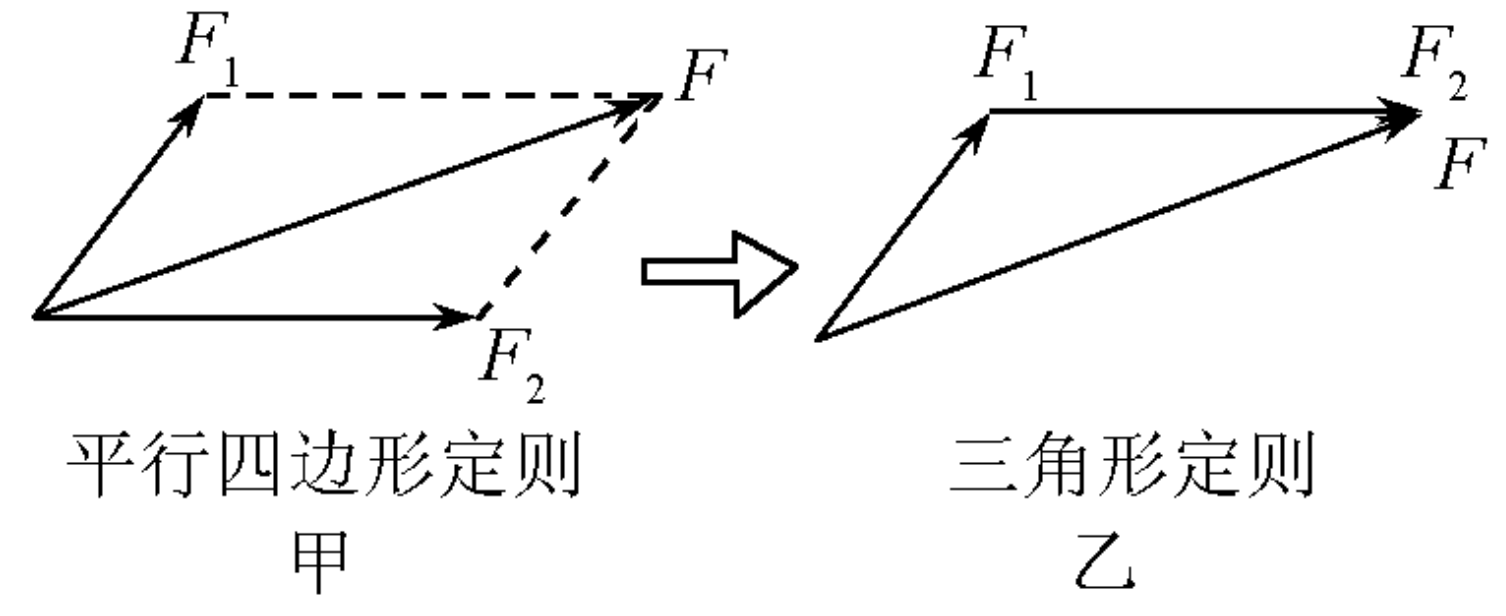
\includegraphics[scale=.3]{vectoradd.png}
  \caption{平行四边形法则与三角形法则}
  \label{fig:vectoradd}
\end{figure}

两个向量相加时,以表示这两个向量的线段为邻边作平行四边形,这两个邻边之间的对角线就代表向量和的大小和方向,这就叫做\textbf{平行四边形定则(Parallelogram law)}。

\textbf{三角形法则(Triangle law)}是指两个向量,将一个向量的起点移动到另一个向量的终点时,向量和为从未移动向量的起点指向所移动向量的终点的向量。三角形法则适用于多个向量求和,只需要将向量按照相加顺序依次首尾排列,第一个向量的起点指向最后一个向量的终点的向量就是求和的结果。

在代数上,对于在笛卡尔坐标系中定义的向量,向量求和可以简化为求向量各个对应坐标值的和。

\subsection{笛卡尔坐标系}
在数学里,\textbf{笛卡尔坐标系 (Cartesian coordinate system)},亦称直角坐标系,是一种正交坐标系。二维的直角坐标系是由两条相互垂直,相交于原点的数线构成的。在平面内,任何一点的坐标是根据数轴上对应的点的坐标设定的。对于向量,我们认为所有向量都是以原点为起点,那么终点的坐标就可以表示一个唯一的向量。

在计算机图形学中,我们默认所有的向量都是列向量,用符号表示向量,向量的转置以及向量的模如下:

\begin{equation}
A=\begin{pmatrix}
x\\ 
y
\end{pmatrix}
\end{equation}
\begin{equation}
A^T=(x,y)
\end{equation}
\begin{equation}
||A||=\sqrt{x^2+y^2}
\end{equation}

\subsection{向量乘法}

\subsubsection{点乘}

\textbf{点乘(Dot product)},又称为向量的内积。计算公式为:
\begin{equation}
	\overrightarrow{a} \cdot \overrightarrow{b} = ||\overrightarrow{a}||||\overrightarrow{b}||\cos\theta
\end{equation}

点乘满足交换律以及分配律。

\begin{equation}
	\overrightarrow{a} \cdot \overrightarrow{b} = \overrightarrow{b} \cdot \overrightarrow{a}\ \text{(交换律)}
\end{equation}


\begin{equation}
	\overrightarrow{a} \cdot (\overrightarrow{b}+\overrightarrow{c}) = \overrightarrow{a} \cdot \overrightarrow{b}+\overrightarrow{a} \cdot \overrightarrow{c}\ \text{(分配律)}
\end{equation}

在笛卡尔坐标系下点乘的计算结果是逐坐标元素相乘后相加的结果。

在2维情况下:

\begin{equation}
	\overrightarrow{a} \cdot \overrightarrow{b} = \begin{pmatrix}
		x_a\\ 
		y_a
	\end{pmatrix}\cdot
	\begin{pmatrix}
		x_b\\ 
		y_b
	\end{pmatrix}
	=x_ax_b+y_ay_b
\end{equation}

在3维情况下:

\begin{equation}
	\overrightarrow{a} \cdot \overrightarrow{b} = \begin{pmatrix}
		x_a\\ 
		y_a\\
		z_a
	\end{pmatrix}\cdot
	\begin{pmatrix}
		x_b\\ 
		y_b\\
		z_b
	\end{pmatrix}
	=x_ax_b+y_ay_b+z_az_b 
\end{equation}

\textbf{点乘的应用:}
\begin{enumerate}[1)]
	\item 计算两个向量的夹角;
	
	通过原公式我们可以推出:
	\begin{equation}
	\cos\theta=\frac{\overrightarrow{a}\cdot\overrightarrow{b}}{||\overrightarrow{a}||||\overrightarrow{b}||}
	\end{equation}

	当两个向量都是单位向量时,我们可以得出更为简单的公式:
	\begin{equation}
		\cos\theta=\hat{a}\cdot\hat{b}
	\end{equation}
	
	我们可以求出两个向量夹角的余弦值,从而得到两个向量的夹角大小。
	
	\item 计算一个向量到另一个向量上的投影;
	
	向量$\overrightarrow{b}$在向量$\overrightarrow{a}$上的投影满足:
	\begin{equation}
		\overrightarrow{b}_\perp=k\hat{a}
	\end{equation}

	$k$的大小为:$k = ||\overrightarrow{b}_\perp||=||\overrightarrow{b}||\cos\theta$.已知两个向量的内积,一个向量在另一个向量上的投影长度为:
	\begin{equation}
		k=||\overrightarrow{b}||\cos\theta=\frac{\overrightarrow{a}\cdot\overrightarrow{b}}{||\overrightarrow{a}||}
	\end{equation}

	\item 计算两个向量的接近程度;
	
	根据$\cos$在角度$[0,\pi]$之间的值可以得出结论,越接近(夹角比较小)的两个向量的单位向量点乘结果越接近于1,反之越远离(夹角比较大)的两个向量的单位向量点乘结果越接近于-1.
	
	\item 计算两个向量的方向是相同还是相反的。
	
	首先我们定义两个向量的方向相同或者相反。如图所示,向量$\overrightarrow{a}$以其垂线为分界,在上半部分(上半圆)的向量认为和向量$\overrightarrow{a}$方向基本相同,在下半部分(下半圆)的向量认为和向量$\overrightarrow{a}$方向基本相反。
	\begin{figure}[H]
		\centering
		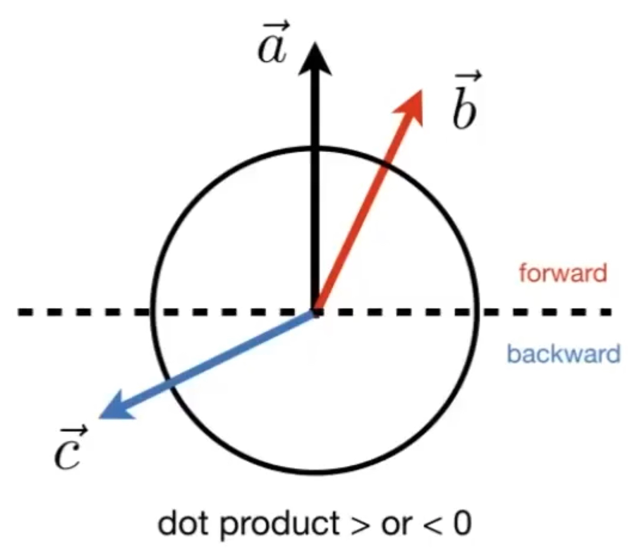
\includegraphics[scale=.25]{vectordirection.png}
		\caption{向量的方向}
		\label{fig:vectordir}
	\end{figure}

	如果两个向量方向基本相同,那么点乘的结果大于0;如果两个向量的方向基本相反,点乘的结果小于0;如果两个向量是垂直的,那么点乘的结果等于0.
	
	
\end{enumerate}

\subsubsection{叉乘}

\textbf{叉乘(Cross product)},又称作向量的外积。两个向量叉乘的结果还是一个向量,这个向量和原来的两个向量垂直。叉乘的结果向量的长度为:
\begin{equation}
	||a\times b||=||a||||b||\sin\phi
\end{equation}

结果向量的方向满足\textbf{右手定则}.右手定则指的是,使用右手的四指从第一个向量到第二个向量握拳,大拇指指向的方向是叉乘结果向量的方向。因此叉乘不满足交换律。

\begin{figure}[H]
	\centering
	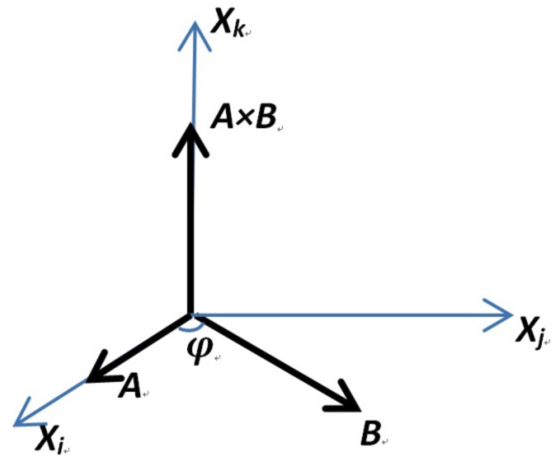
\includegraphics[scale=.25]{crossproduct.png}
	\caption{叉乘}
	\label{fig:corssproduct}
\end{figure}

叉乘满足分配律,以及数乘结合律。向量自己和自己的叉乘结果是0.

在笛卡尔坐标系的表示下进行叉乘计算的结果可以写作:
\begin{equation}
	\overrightarrow{a} \times \overrightarrow{b} = \begin{pmatrix}
		y_az_b-y_bz_a\\ 
		z_ax_b-x_az_b\\
		x_ay_b-y_ax_b
	\end{pmatrix}
\end{equation}

我们可以将向量$	\overrightarrow{a}$写成等价的矩阵形式:
\begin{equation}
	\overrightarrow{a} \times \overrightarrow{b} = 
	A*b=\begin{pmatrix}
		0&-z_a&y_a\\
		z_a& 0& -x_a\\
		-y_a & x_a & 0
	\end{pmatrix} 
	\begin{pmatrix}
		x_b\\
		y_b\\
		z_b
	\end{pmatrix} 
\end{equation}

\textbf{叉乘的应用}

\begin{enumerate}[1)]
	\item 判断一个向量在另一个向量的左边还是右边;
	
	一个向量对另一个向量做叉乘,如果说结果方向为正,那么另一个向量在这个向量的右边。如果结果为负,那么在左边。
	
	\item 判定一个点在三角形的内部还是外部。
	\begin{figure}[H]
		\centering
		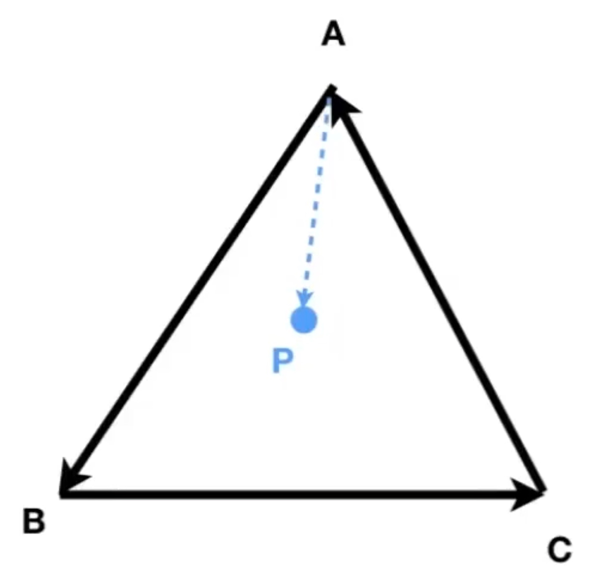
\includegraphics[scale=.25]{corssinout.png}
		\caption{判断点是否在三角形内部}
		\label{fig:corssio}
	\end{figure}

	只要P点在边AB,BC,AC(注意输入顺序)的左边,那么就满足P点在三角形ABC中。那么可以对每个边分别求一次叉乘判断点是否在三角形内部。三角形的输入必须保证为顺时针或者逆时针。为了忽略顺时针和逆时针的差别(顺时针输入需要要求点在三角形每一条边的右边),只要P在都在每条边的左边或者每条边的右边都算作在三角形内部。对于边界情况(如果叉乘结果为0),那么由自己根据实际问题定义这是内部还是外部。
	
\end{enumerate}

\section{正交系/坐标系}

\textbf{右手坐标系(right-hand system)}的定义如下。我们定义三个坐标轴$\overrightarrow{u}$,$\overrightarrow{v}$,$\overrightarrow{w}$满足以下性质:
\begin{equation}
	||\overrightarrow{u}||=||\overrightarrow{v}||=||\overrightarrow{w}||=1
\end{equation}

\begin{equation}
	\overrightarrow{u}\cdot\overrightarrow{v}=\overrightarrow{v}\cdot\overrightarrow{w}=\overrightarrow{u}\cdot\overrightarrow{w}=0
\end{equation}

\begin{equation}
	\overrightarrow{w}=\overrightarrow{u}\times\overrightarrow{v}\ \text{(右手定则)}
\end{equation}

那么向量$\overrightarrow{u}$,$\overrightarrow{v}$,$\overrightarrow{w}$定义了一个右手坐标系。对于任意一个向量$\overrightarrow{p}$,在右手坐标系中可以表示为:
\begin{equation}
	\overrightarrow{p}=(\overrightarrow{p}\cdot \overrightarrow{u})\overrightarrow{u}+(\overrightarrow{p}\cdot \overrightarrow{v})\overrightarrow{v}+(\overrightarrow{p}\cdot \overrightarrow{w})\overrightarrow{w}
\end{equation}

\section{矩阵}

\textbf{矩阵(Matrix)},是一个按照长方阵列$m\times n$排列的复数或实数集合。

\subsection{矩阵乘法}

矩阵乘法$A\times B$必须满足$A$的列数=$B$的行数。求出的矩阵的大小为:
\begin{equation}
	(m\times n)(n\times p) = (m\times p)
\end{equation}

矩阵乘法不满足交换律,但是满足结合律和分配律。

矩阵和向量相乘时,认为向量是一个列向量并乘在矩阵的右边。

矩阵也有转置,并且矩阵乘法转置满足$(AB)^T=B^TA^T$.

\textbf{单位矩阵}是一个左上到右下对角线值为1,其他值为0的正方形矩阵,以长度为3的单位矩阵为例:

\begin{equation}
	I_{3\times 3}=\begin{pmatrix}
		1&0&0\\
		0&1&0\\
		0&0&1
	\end{pmatrix}
\end{equation}

单位矩阵定义了矩阵的逆运算。对于矩阵$A$来说,矩阵的逆$A^{-1}$满足:
\begin{equation}
	AA^{-1}=A^{-1}A=I
\end{equation}

矩阵乘法的逆满足:
\begin{equation}
	(AB)^{-1}=B^{-1}A^{-1}
\end{equation}

\chapter{变换}

\textbf{变换(Transform)}是计算机图形学中非常重要的一部分。变换包含模型变换(Modeling transform)以及视图变换(View transform)。模型变换指的是变换模型(被拍摄物体)的位置,大小和角度;视图变换指的是变换照相机的位置和角度。从相对运动的角度来看,两种变换是可以相互转化的。

\section{模型变换}

\subsection{2维变换}

\subsubsection{缩放变换}

缩放变换(Scale)中,如果一个图片以原点$(0,0)$为中心缩放$s$倍。那么点$(x,y)$变换后数学形式可以表示为:

\begin{equation}
\begin{split}
	x'=sx
	\\
	y'=sy
\end{split}
\end{equation}

写成矩阵形式为:
\begin{equation}
	\begin{bmatrix}
		x' \\
		y'
	\end{bmatrix} = \begin{bmatrix}
		s&0\\0&s\end{bmatrix}\begin{bmatrix}x\\y\end{bmatrix}
\end{equation}

当然,我们也可以给x轴和y轴不同的缩放倍数$s_x$和$s_y$。在非均匀情况下,缩放变换的矩阵形式为:
\begin{equation}
	\begin{bmatrix}
		x' \\
		y'
	\end{bmatrix} = \begin{bmatrix}
		s_x&0\\0&s_y\end{bmatrix}\begin{bmatrix}x\\y\end{bmatrix}
\end{equation}

\subsubsection{反射变换}

反射变换(Reflection)指的是图片对着x轴或者y轴做对称变换。对于图片上的点$(x,y)$在经过x轴的对称反射变换后,数学形式可以表示为:
\begin{equation}
	\begin{split}
		x'=-x\\y'=y
	\end{split}
\end{equation}

表示成矩阵形式为:
\begin{equation}
	\begin{bmatrix}
	x' \\
	y'
\end{bmatrix} = \begin{bmatrix}
-1&0\\0&1\end{bmatrix}\begin{bmatrix}x\\y\end{bmatrix}
\end{equation}

同理可以得到y轴对称反射变换后的变换矩阵为:

\begin{equation}
	\begin{bmatrix}
		x' \\
		y'
	\end{bmatrix} = \begin{bmatrix}
		1&0\\0&-1\end{bmatrix}\begin{bmatrix}x\\y\end{bmatrix}
\end{equation}

沿原点反射变换的变换矩阵为:

\begin{equation}
	\begin{bmatrix}
		x' \\
		y'
	\end{bmatrix} = \begin{bmatrix}
		-1&0\\0&-1\end{bmatrix}\begin{bmatrix}x\\y\end{bmatrix}
\end{equation}

\subsubsection{切变变换}

\textbf{切变变换(Shear)},指的是在物理学上指的是两个距离很近、大小相等、方向相反的平行力作用于同一物体上所引起的形变。使用示意图可以更直观的去表示什么是切变。如图\ref{fig:shear}所示,是图片在x轴方向上发生了切变。从图中我们可以看出所有点在y轴上的坐标不变,在x轴上的坐标满足:$y=0$上的点,x轴坐标不发生变化;$y=1$上的点水平方向上移动了$a$个长度。因此对于任意一个点来说,水平方向上移动长度为$ay$。

\begin{figure}[H]
	\centering
	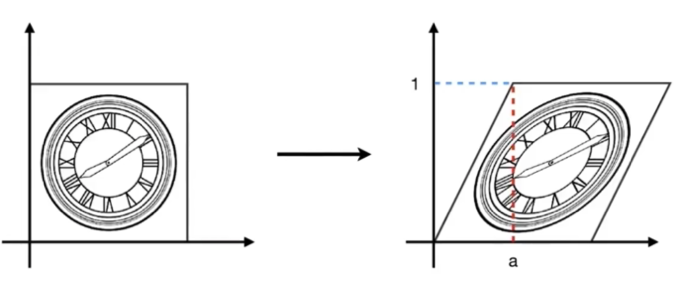
\includegraphics[scale=.25]{shear.png}
	\caption{切变变换}
	\label{fig:shear}
\end{figure}

切变的矩阵变换可以写作:
\begin{equation}
	\begin{bmatrix}x'\\y'\end{bmatrix}=\begin{bmatrix}1&a\\0&1\end{bmatrix}\begin{bmatrix}x\\y\end{bmatrix}
\end{equation}

\subsubsection{旋转变换*}

我们默认\textbf{旋转变换(Rotate)}都绕着原点$(0,0)$旋转,并且默认旋转方向为逆时针方向(逆时针方向旋转角度值为正,顺时针旋转角度值为负)。旋转变换的推导过程比较复杂(见后续推导过程)。结论如下:当一个点$(x,y)$绕着原单$(0,0)$旋转$\theta$角时,变换矩阵可以表示为:

\begin{equation}
	\begin{bmatrix}x'\\y'\end{bmatrix}=\begin{bmatrix}\cos\theta&-\sin\theta\\\sin\theta&\cos\theta\end{bmatrix}\begin{bmatrix}x\\y\end{bmatrix}
\end{equation}

\begin{titledbox}{旋转变换矩阵的推导过程}
	\begin{figure}[H]
		\centering
		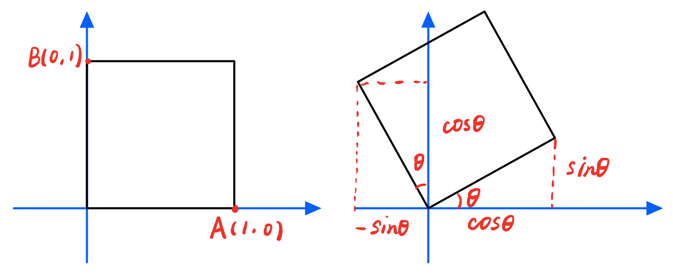
\includegraphics[scale=.25]{rotate.png}
		\caption{旋转变换的推导}
		\label{fig:shear}
	\end{figure}

我们在直角坐标系中绘制一个边长为1的正方形,点$A$坐标为$(1,0)$,点$B$坐标为$(0,1)$。正方形沿着原点$(0,0)$旋转的角度为$\theta$角。我们设:

\begin{equation}
	\begin{bmatrix}x'\\y'\end{bmatrix}=\begin{bmatrix}A&B\\C&D\end{bmatrix}\begin{bmatrix}x\\y\end{bmatrix}
\end{equation}

代入点$A$的的值$(1,0)$可以得到:
\begin{equation}
	\begin{bmatrix}\cos\theta\\\sin\theta\end{bmatrix}=\begin{bmatrix}A&B\\C&D\end{bmatrix}\begin{bmatrix}1\\0\end{bmatrix}
\end{equation}

解方程得到:

\begin{equation}
\begin{split}
	A=\cos\theta\\C=\sin\theta
\end{split}
\end{equation}

代入点$B$的的值$(0,1)$可以得到:
\begin{equation}
	\begin{bmatrix}-\sin\theta\\\cos\theta\end{bmatrix}=\begin{bmatrix}A&B\\C&D\end{bmatrix}\begin{bmatrix}0\\1\end{bmatrix}
\end{equation}

解方程得到:

\begin{equation}
	\begin{split}
		B=-\sin\theta\\D=\cos\theta
	\end{split}
\end{equation}

因此:
\begin{equation}
	M_{rotate}=\begin{bmatrix}\cos\theta&-\sin\theta\\\sin\theta&\cos\theta\end{bmatrix}
\end{equation}

\end{titledbox}

\subsubsection{线性变换}

对于任何一种变换如果可以写作:
\begin{equation}
	\begin{split}
		x'=ax+by\\y'=cx+dy
	\end{split}
\end{equation}

矩阵形式可以表示为:
\begin{equation}
	\begin{split}
	\begin{bmatrix}x'\\y'\end{bmatrix}=\begin{bmatrix}a&b\\c&d\end{bmatrix}\begin{bmatrix}x\\y\end{bmatrix}
	\\
	x'=Mx
	\end{split}
\end{equation}

那么我们认为这种变换是\textbf{线性变换(Linear transformation)}。

\subsection{齐次坐标}

\subsubsection{平移变换}

\textbf{平移变换(Translation)}相比于以上的线性变换有特殊的地方。平移变换的数学形式为:
\begin{equation}
	\begin{split}
		x'=x+t_x\\
		y'=y+t_y
	\end{split}
\end{equation}

这种数学表示不能写作线性变换的矩阵形式,只能记作:
\begin{equation}
	\begin{bmatrix}x'\\y'\end{bmatrix}=\begin{bmatrix}a&b\\c&d\end{bmatrix}\begin{bmatrix}x\\y\end{bmatrix}+\begin{bmatrix}t_x\\t_y\end{bmatrix}
\end{equation}

说明平移操作\textbf{不是}线性变换。但是我们不希望把平移操作看作特殊变换,因此需要把这些变换统一起来,就引入了齐次坐标。

\subsubsection{齐次坐标的引入}

为了统一变换操作,我们引入一个新的维度。对于二维的点$(x,y)$我们可以增加一个维度,对于2维的点可以表示为$(x,y,1)^T$,2维向量的$(x,y,0)^T$。因此,一个点的平移可以用矩阵表示为:
\begin{equation}
	\begin{bmatrix}x'\\y'\\w'\end{bmatrix}=\begin{bmatrix}1&0&t_x\\0&1&t_y\\0&0&1\end{bmatrix}\begin{bmatrix}x\\y\\1\end{bmatrix}=\begin{bmatrix}x+t_x\\y+t_y\\1\end{bmatrix}
\end{equation}

\begin{question}
	\textbf{为什么点补充维度大小为1,但是向量补充维度大小为0?}
	
	对于向量来说,平移变换不应该使向量的结果发生变化。因此补充维度为0的时候可以屏蔽平移带来的影响。
	
	对于加入齐次坐标的点和向量满足:
	\begin{enumerate}
		\item 向量+向量=向量
		\item 点-点=向量
		\item 点+向量=点
		\item 点+点=\textbf{两个点中点}
		
			对引入齐次坐标的点的扩充定义如下:
			\begin{equation}
				\begin{pmatrix}x\\y\\w\end{pmatrix}=\begin{pmatrix}x/w\\y/w\\1\end{pmatrix},w\ne 0
			\end{equation}
			因此一个点加上另一个点的结果是两个点的\textbf{中点}。引入了扩充定义点和向量的加法是有意义的。
	\end{enumerate}
\end{question}

\subsection{仿射变换}

\textbf{仿射变换(Affine)}包含线性变换与平移变换。可以用矩阵表示为:

\begin{equation}
	\begin{bmatrix}x'\\y'\end{bmatrix}=\begin{bmatrix}a&b\\c&d\end{bmatrix}\begin{bmatrix}x\\y\end{bmatrix}+\begin{bmatrix}t_x\\t_y\end{bmatrix}
\end{equation}

使用齐次坐标后可以写作:

\begin{equation}
	\begin{bmatrix}x'\\y'\\w'\end{bmatrix}=\begin{bmatrix}a&b&t_x\\c&d&t_y\\0&0&1\end{bmatrix}\begin{bmatrix}x\\y\\1\end{bmatrix}=\begin{bmatrix}ax+by+t_x\\cx+dy+t_y\\1\end{bmatrix}
\end{equation}

\subsection{逆变换}

任何变换的\textbf{逆变换(Inverse transform)}的变换矩阵$M$的逆矩阵$M^{-1}$表示。

\subsection{变换的组合与分解}

\subsubsection{变换的组合}

可以用\textbf{矩阵的乘法}进行变换的组合(Transform compose)。变换的先后顺序不同,变换的结果不同。矩阵和向量的乘法是从右到左依次相乘,从右到左依次应用变化。如果我们要依次应用变化$A_1,A_2,A_3,\cdots$,写成矩阵形式:

\begin{equation}
	A_n(\dots A_2(A_1(x)))=A_n\dots A_2\cdot A_1\cdot \begin{pmatrix}x\\y\\1\end{pmatrix}
\end{equation}

根据矩阵运算的\textbf{结合律},我们可以先把变换矩阵乘在一起,接下来把这个矩阵的乘积和向量相乘。可以用一个矩阵表示一个复杂的变换。

\subsubsection{变换的分解}

所有的复杂变换都可以分解成多个普通的变换。为了使某个图像沿着某个点$c$变换,我们可以分解为以下步骤:

\begin{enumerate}
	\item 把中心点$c$移动到原点;
	\item 进行旋转;
	\item 把中心点$c$平移到原点;
\end{enumerate}

用变换矩阵表示为:
\begin{equation}
	M_{t}(c)\cdot M_{r}(\theta) \cdot M_{t}(-c)
\end{equation}

\subsection{3维变换}

3维变换可以类比于2维变换得到引入齐次坐标的点和向量,3维的点可以表示为$(x,y,z,1)^T$,3维向量可以表示为$(x,y,z,0)^T$。当$w\ne 0$的时候:
\begin{equation}
	(x,y,z,w)=(x/w,y/w,z/w,1)
\end{equation}

使用$4\times 4$的矩阵来表示仿射变换:

\begin{equation}
	\begin{pmatrix}x'\\y'\\z'\\1\end{pmatrix}=\begin{pmatrix}a&b&c&t_x\\d&e&f&t_y\\g&h&i&t_z\\0&0&0&1\end{pmatrix}\cdot\begin{pmatrix}x\\y\\z\\1\end{pmatrix}
\end{equation}

左上角是一个$3\times 3$的线性变换矩阵。

在仿射变换中的变换矩阵表示先\textbf{线性变换}再\textbf{平移}。

\subsubsection{3维变换中缩放变换}
3维变换中缩放变换的变换矩阵:
\begin{equation}
	\textbf{S}(s_x,s_y,s_z)=\begin{pmatrix}s_x&0&0&0\\0&s_y&0&0\\0&0&s_z&0\\0&0&0&1\end{pmatrix}
\end{equation}

\subsubsection{3维变换中的平移变换}
3维变换中平移变换的变换矩阵:
\begin{equation}
	\textbf{T}(t_x,t_y,t_z)=\begin{pmatrix}1&0&0&t_x\\0&1&0&t_y\\0&0&1&t_z\\0&0&0&1\end{pmatrix}
\end{equation}

\subsubsection{3维变换中的旋转变换}

当空间内的物体绕着x轴,y轴或者z轴旋转的时候,变换矩阵为:

\begin{equation}
\textbf{R}_x(\alpha)=\begin{pmatrix}1&0&0&0\\0&\cos\alpha&-\sin\alpha&0\\0&\sin\alpha&\cos\alpha&0\\0&0&0&1\end{pmatrix}
\end{equation}

\begin{equation}
	\textbf{R}_y(\alpha)=\begin{pmatrix}\cos\alpha&0&\sin\alpha&0\\0&1&0&0\\-\sin\alpha&0&\cos\alpha&0\\0&0&0&1\end{pmatrix}
\end{equation}

\begin{equation}
	\textbf{R}_z(\alpha)=\begin{pmatrix}\cos\alpha&-\sin\alpha&0&0\\\sin\alpha&\cos\alpha&0&0\\0&0&1&0\\0&0&0&1\end{pmatrix}
\end{equation}

\begin{question}
	\textbf{为什么$\textbf{R}_y$的$\sin\alpha$的符号位置是反的?}
	
	因为只有y轴按照右手法则是$zx=y$,x轴和z轴的顺序是反的。所以我规定从z轴到x轴旋转为逆时针方向的情况下,$\sin\alpha$的负号位置应该在z轴对应的这一行。也可以理解为对角线上的循环移动。
\end{question}

对于一般性的旋转问题,可以用简单的旋转描述复杂的旋转。用x轴,y轴和z轴上的旋转来定义旋转:
\begin{equation}
	\textbf{R}_{xyz}(\alpha,\beta,\gamma)=\textbf{R}_x(\alpha)\textbf{R}_y(\beta)\textbf{R}_z(\gamma)
\end{equation}

这三个角就被称作\textbf{欧拉角(Euler angles)}。

\subsubsection{罗德里格斯旋转公式}

绕着旋转轴$\textbf{n}$旋转角度$\alpha$。默认旋转轴是过原点的,对于不过原点的条件可以将图形平移到过原点的旋转轴上,旋转后再平移回去。罗德里格斯旋转公式(Rodrigues' Rotation Formula)是:
\begin{equation}
	\textbf{R}(\textbf{n},\alpha)=\cos(\alpha)\textbf{I}+(1-\cos(\alpha))\textbf{n}\textbf{n}^T+\sin(\alpha)\begin{pmatrix}0&-n_z&n_y\\n_z&0&-n_x\\-n_y&n_x&0\end{pmatrix}
\end{equation}

最后的矩阵一般记作$N$,矩阵$N$满足叉乘的矩阵形式。

%\begin{titledbox}{罗德里格斯旋转公式的证明}
%	
%	
%\end{titledbox}

\section{视图变换}

在3维物体变到二维平面的过程中,我们需要规定好相机的位置。对于相机所做的变换就是\textbf{视图变换(Viewing/Camera transformation)}。

我们需要对相机位置进行定义,对于一个相机我们要规定下面三个属性:
\begin{enumerate}
	\item 相机位置(Position)$\overrightarrow{e}$
	\item 相机拍摄方向(Look-at/Gaze direction)$\hat{g}$
	\item 相机向上方向(Up direction,假设垂直于look-at direction)$\hat{t}$
\end{enumerate}

根据相对运动我们可以知道,只要相机和被拍摄物体相对位置不变,那么拍摄出来的照片应当是一样的。我们可以通过对被拍摄物体做相同的变换来把相机变换到标准位置。相机的标准位置为:
\begin{enumerate}
	\item 相机位置在原点$(0,0)$;
	\item 相机拍摄方向是-z轴方向;
	\item 相机的向上方向是y轴方向。
\end{enumerate}

将任意位置的相机移动到标准位置需要以下操作:

\begin{enumerate}
	\item 将中心点$\overrightarrow{e}$移动到原点;
	\item 把$\hat{g}$旋转到-z轴方向;
	\item 把$\hat{t}$旋转到y轴方向;
	\item 把$\hat{g}\times\hat{t}$旋转到x轴方向。
\end{enumerate}

操作2~4只要满足任意两个,另外一个条件就会满足。也就是说我们需要先做一次平移变换,再做一次旋转变换。

平移变换的变换矩阵可以写作:

\begin{equation}
	T_{view}=\begin{pmatrix}1&0&0&-x_e\\0&1&0&-y_e\\0&0&1&-z_e\\0&0&0&1\end{pmatrix}
\end{equation}

旋转矩阵的写法比较麻烦。从$\hat{g}$旋转到-z轴方向,$\hat{t}$旋转到y轴方向以及$\hat{g}\times\hat{t}$旋转到x轴方向比较难写,但是旋转变换的逆变换非常的简单:

\begin{equation}
	R^{-1}_{view}=\begin{pmatrix}x_{\hat{g}\times\hat{t}}&x_t&x_{-g}&0\\y_{\hat{g}\times\hat{t}}&y_t&y_{-g}&0\\z_{\hat{g}\times\hat{t}}&z_t&z_{-g}&0\\0&0&0&1\end{pmatrix}
\end{equation}

我们用x轴方向单位向量$(1,0,0,0)$,y轴单位向量$(0,1,0,0)$,z轴单位向量$(0,0,1,0)$代入后结果是正确的。我们知道旋转矩阵的逆矩阵是正交矩阵,因此旋转变换矩阵的逆是旋转变换矩阵的转置矩阵。也就是说:

\begin{equation}
	R_{view}=\begin{pmatrix}x_{\hat{g}\times\hat{t}}&y_{\hat{g}\times\hat{t}}&z_{\hat{g}\times\hat{t}}&0\\x_t&y_t&z_t&0\\x_{-g}&y_{-g}&z_{-g}&0\\0&0&0&1\end{pmatrix}
\end{equation}

\begin{information}
	\textbf{旋转变换矩阵是正交矩阵,矩阵的逆等于矩阵的转置。}
	
	旋转$\theta$角的逆变换就是旋转$-\theta$角。旋转$-\theta$角的变换矩阵是:
	\begin{equation}
		R_{-\theta}=\begin{bmatrix}\cos\theta&\sin\theta\\-\sin\theta&\cos\theta\end{bmatrix} = R_{\theta}^T
	\end{equation}

	同时:
	
	\begin{equation}
		R_{-\theta}=R_{\theta}^{-1}\ \text{(by definition)}
	\end{equation}

	旋转矩阵的逆等于旋转矩阵的转置,这样的矩阵被称为正交矩阵。

\end{information}

以上就是我们得到的视图变换矩阵。

\section{投影变换}

\textbf{投影变换(Projection transformation)}是把3维模型投影到2维平面的变换。投影变换分为正交投影(Orthographic projection)以及透视投影(Perspective projection)。正交投影中,投影后原本平行的线保持平行关系。但是透视投影中平行的线在投影后不一定能保持平行关系,会相交到某一点上(这也就是近大远小现象)。

\begin{figure}[H]
	\centering
	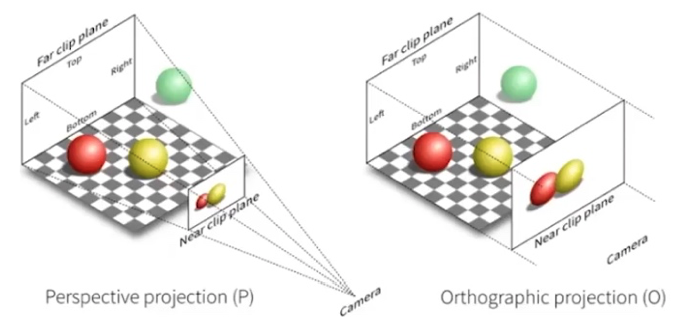
\includegraphics[scale=.4]{projection.png}
	\caption{透视投影与正交投影}
	\label{fig:projection}
\end{figure}

\subsection{正交投影}

正交投影将相机放在原点上,拍摄方向是-z轴方向,向上方向是y轴方向。只需要去掉z轴后,xy平面上的图像就是投影结果。为了能够正交投影,我们会把所有模型移动到$[-1,1]^3$的区间范围内。

在空间中描述一个立方体(立方体中包含了所有需要绘制的模型),将立方体变换到$[-1,1]^3$的区间范围内。

\begin{figure}[H]
	\centering
	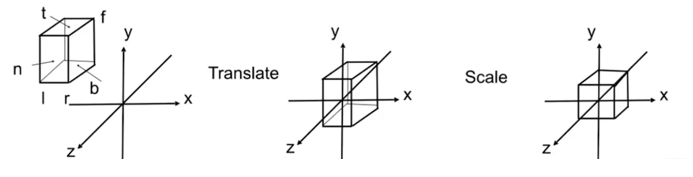
\includegraphics[scale=.4]{orp.png}
	\caption{正交投影变换}
	\label{fig:projection}
\end{figure}

定义空间中的立方体的左右在x轴的坐标,上下在y轴的坐标,远近在z轴的坐标。这个立方体就可以被描述$[l,r]\times[b,t]\times[f,n]$。对于z轴来说,越远z值更小,越近z值更大。远是小于近的,保证了右手坐标系下从-z方向看过去z值的规律。

将这样的立方体映射到正则/标准/规范(canonical)立方体$[-1,1]^3$

变换方法是先将中心平移到原点,之后对每个边进行缩放到大小为2。

变换矩阵为:

\begin{equation}
	M_{ortho}=\begin{pmatrix}\frac{2}{r-l}&0&0&0\\0&\frac{2}{t-b}&0&0\\0&0&\frac{2}{n-f}&0\\0&0&0&1\end{pmatrix}\begin{pmatrix}1&0&0&-\frac{r+l}{2}\\0&1&0&-\frac{t+b}{2}\\0&0&1&-\frac{n+f}{2}\\0&0&0&1\end{pmatrix}
\end{equation}

\subsection{透视投影}

\textbf{透视投影(Perspective projection)}是最为广泛的投影方式。透视投影满足\textbf{近大远小}的性质。接下来我们定义\textbf{视锥}。视锥就是一个透视相机渲染时能看到区域的形状,相机放在平面的中心,一个视锥包含4个元素:

\begin{figure}[H]
	\centering
	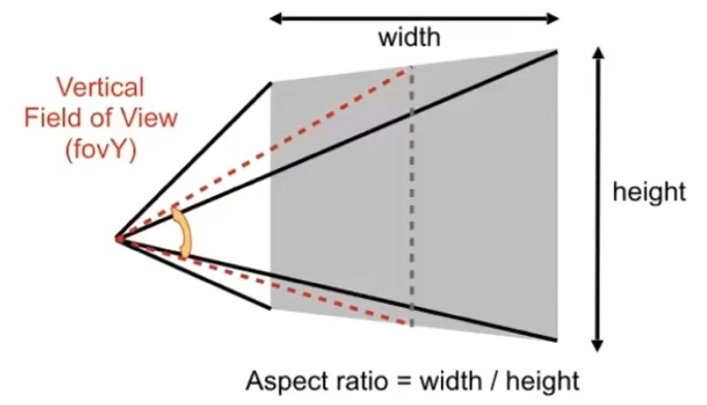
\includegraphics[scale=.3]{shizhui.png}
	\caption{视锥示意图}
	\label{fig:projection}
\end{figure}

\begin{enumerate}
	\item 近平面:渲染的区域里相机最近的平面;
	\item 远平面:渲染的区域里相机最远的平面;
	\item 视野(Field of view,FOV):平面顶部和底部中心到相机连线的夹角;
	\item 宽高比:平面宽度和高度之比。
\end{enumerate}

从一个点射出的四棱锥定义了远和近两个平面。我们可以把远平面缩小成和近平面一样大的长方形,这样视锥就会变成一个立方体。再做一次正交投影就可以得到最终的投影结果了。

\begin{figure}[H]
	\centering
	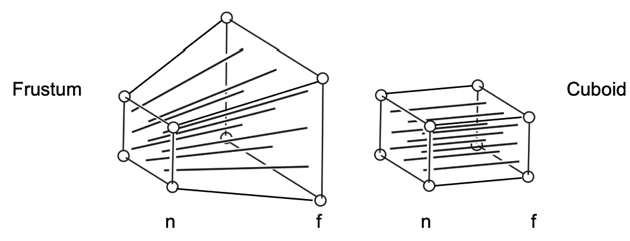
\includegraphics[scale=.4]{toushitouying.png}
	\caption{透视投影变换示意图}
	\label{fig:projection}
\end{figure}

我们需要对这些点进行变换,变换满足三个条件:
\begin{enumerate}
	\item 任何一个在近平面上的点不会发生变化;
	\item 远平面处的点z值不发生变化;
\end{enumerate}

\begin{figure}[H]
	\centering
	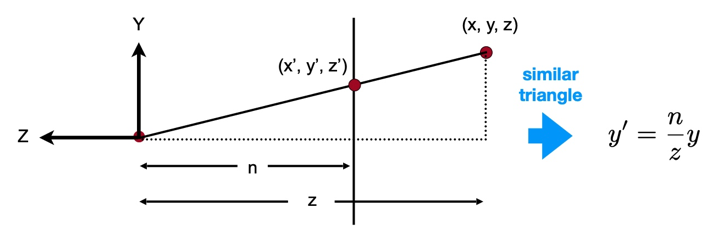
\includegraphics[scale=.4]{bianhuanjisuan.png}
	\caption{透视投影变换YZ平面示意图}
	\label{fig:projection}
\end{figure}

从YZ平面看过去,对于远平面上的点$(x,y,z)$在投影变换后,根据相似三角形的性质,点的位置变为$(\frac{n}{z}x,\frac{n}{z}y,z)$。对于任意一个点点$(x,y,z)$来说,变化过程为:

\begin{equation}
	\begin{pmatrix}x\\y\\z\\1\end{pmatrix}\rightarrow\begin{pmatrix}nx/z\\ny/z\\\text{unknown}\\1\end{pmatrix}==\begin{pmatrix}nx\\ny\\\text{still unknown}\\z\end{pmatrix}
\end{equation}

中间点的z值变化目前是不确定的。但是对于以上的变化结果我们可以得到变换矩阵的部分结果:

\begin{equation}
	M_{persp\rightarrow ortho}=\begin{pmatrix}n&0&0&0\\0&n&0&0\\?&?&?&?\\0&0&1&0\end{pmatrix}
\end{equation}

接下来求出未知量。对于近平面的上的点,应当满足变换:

\begin{equation}
	\begin{pmatrix}x\\y\\n\\1\end{pmatrix}\rightarrow\begin{pmatrix}x\\y\\n\\1\end{pmatrix}==\begin{pmatrix}nx\\ny\\n^2\\n\end{pmatrix}
\end{equation}

因此可以得到方程:

\begin{equation}
	\begin{pmatrix}0&0&A&B\end{pmatrix}\begin{pmatrix}x\\y\\n\\1\end{pmatrix}=n^2
\end{equation}

$n^2$显然和x,y的值没有什么关系,因此x,y的系数为0。但是方程不能解出,还需要一个方程。

对于远平面,我们选择中心点,变换应当满足:

\begin{equation}
	\begin{pmatrix}0\\0\\f\\1\end{pmatrix}\rightarrow\begin{pmatrix}0\\0\\f\\1\end{pmatrix}==\begin{pmatrix}0\\0\\f^2\\f\end{pmatrix}
\end{equation}

可以得到方程:

\begin{equation}
	\begin{pmatrix}0&0&A&B\end{pmatrix}\begin{pmatrix}0\\0\\f\\1\end{pmatrix}=f^2
\end{equation}

方程展开后可以得到:

\begin{equation}
	\begin{split}
		An+B=n^2\\
		Af+B=f^2
	\end{split}
\end{equation}

解得:

\begin{equation}
	\begin{split}
		A=n+f\\
		B=-nf
	\end{split}
\end{equation}

因此我们就解出了变换矩阵:

\begin{equation}
	M_{persp\rightarrow ortho}=\begin{pmatrix}n&0&0&0\\0&n&0&0\\0&0&n+f&-nf\\0&0&1&0\end{pmatrix}
\end{equation}

\begin{titledbox}{透视投影的变换后的正交投影变换矩阵}
	对于定义好的视锥,我们定义视野角度为$\alpha$,宽高比为$radio$,近平面z值为$n$,那么投影变换后的长方体的中$t=n\tan{\alpha/2}, b=-n\tan{\alpha/2}, r=radio*n\tan{\alpha/2},l=-radio*n\tan{\alpha/2}$.代入正交投影变化公式中即可。
\end{titledbox}

\begin{question}
	\textbf{中间点在经过透视投影变换后会变得更近还是更远?(以视锥的中间点计算为例)}
	
	计算点$(0,0,\frac{n+f}{2},1)$变换后的位置:
	
	\begin{equation}
		\begin{pmatrix}n&0&0&0\\0&n&0&0\\0&0&n+f&-nf\\0&0&1&0\end{pmatrix}\begin{pmatrix}0\\0\\\frac{n+f}{2}\\1\end{pmatrix} = \begin{pmatrix}0\\0\\\frac{n^2+f^2}{2}\\\frac{n+f}{2}\end{pmatrix} =  \begin{pmatrix}0\\0\\\frac{n^2+f^2}{n+f}\\1\end{pmatrix}
	\end{equation}

	我们可以推算出$\frac{n^2+f^2}{n+f}\ge\frac{n+f}{2}$,因此中间点在经过透视投影后变近了。
\end{question}

\chapter{概率论基础}

本章内容主要介绍概率论相关基础知识,本章数学知识将在第十三章进行使用。

\begin{itemize}
	\item \textbf{随机变量}表示随机试验各种结果的实值单值函数,记做$X$;
	\item \textbf{随机变量的分布}指的是对于随机变量得到某个值的概率;
	\item \textbf{概率}反映随机事件出现的可能性大小,概率$p$满足:$p_i\ge 0,\sum_{i=1}^{n}p_i=1$;
	\item \textbf{期望}指的是是试验中每次可能结果的概率乘以其结果的总和,反映随机变量平均取值的大小;
	\item \textbf{连续变量下的概率密度}等于一段区间(事件的取值范围)的概率除以该段区间的长度;
	\item \textbf{连续变量的期望计算}:$E[X]=\int xp(x)dx$;
	\item 如果$X\sim p(x)$并且$Y=f(X)$,那么$Y$的期望为$E[Y]=E[f(X)]=\int f(x)p(x)dx$.
\end{itemize}


\part{光栅化}

\chapter{光栅化}

我们需要将上一节$[-1,1]^3$的立方体内的物体绘制到屏幕上,我们对屏幕的定义如下:

\begin{enumerate}
	\item 屏幕是像素的数组;
	\item 分辨率是屏幕像素数组的尺寸;
	\item 屏幕是光栅成像设备。
\end{enumerate}

\textbf{光栅化(Rasterization)}指的是将物体绘制到屏幕上。\textbf{像素(Pixel)}是具有统一颜色的小方块,是由不同颜色组合而成的(例如RGB)。

\section{屏幕空间}

\begin{figure}[H]
	\centering
	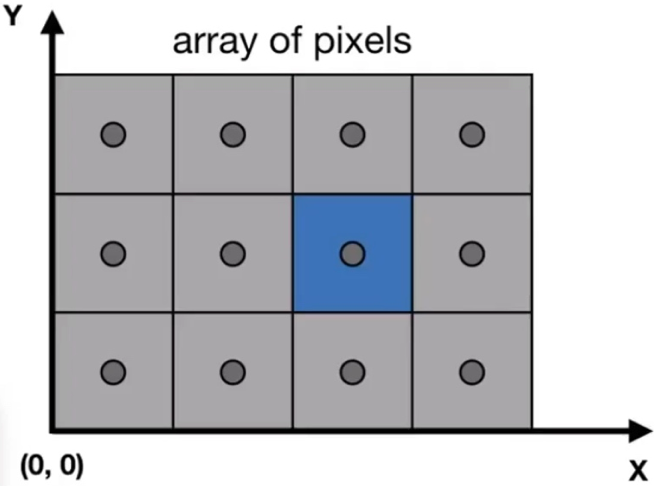
\includegraphics[scale=.3]{pingmukongjian.png}
	\caption{屏幕空间示意图}
	\label{fig:projection}
\end{figure}

我们认为屏幕左下角为原点,向右为x轴,向上为y轴。建立平面直角坐标系。屏幕空间满足以下几点:

\begin{enumerate}
	\item 我们认为像素坐标$(x,y)$为整数坐标;
	\item 像素坐标覆盖范围为$(0,0)$到$(\text{width}-1,\text{height}-1)$;
	\item 像素的中心点在$(x+0.5,y+0.5)$;
	\item 整个屏幕的覆盖范围在$(0,0)-(\text{width}, \text{height})$.
\end{enumerate}

我们需要从$[-1,1]^2$变换到$[0,\text{width}]\times[0,\text{height}]$。这里只需要一个拉伸变换,变换矩阵为:

\begin{equation}
	M_{viewpoint}=\begin{pmatrix}
		\frac{width}{2} &0&0&\frac{width}{2}\\
		0&\frac{height}{2}&0&\frac{height}{2}\\
		0&0&1&0\\
		0&0&0&1
	\end{pmatrix}
\end{equation}

\section{三角形的光栅化}

对于一个3维图形我们可以用三角形去表示一个一个小面。使用三角形的主要原因是:

\begin{itemize}
	\item 三角形是最基本的多边形;
	\item 任何多边形都可以拆分成三角形;
	\item 空间内任何三个点的连线一定是平面;
	\item 三角形由清晰的内部和外部定义;
	\item 三角形只要定义顶点的属性就可以计算三角形内部点的渐变关系(三角形的内部插值)。
\end{itemize}

对于一个三角形,如何映射在像素空间上问题,可以转换成判断一个像素和三角形的位置关系。最简单的方法就是进行\textbf{离散化(Sampling)}。采样就是连续函数的离散化过程。代码表示如下:

\begin{lstlisting}]
for(int x = 0; x < max; ++x)
	output[x]=f(x);
\end{lstlisting}
我们对于给定三角形,判断像素中心是否在三角形内部。如果在,那么这个点为1,否则为0.

\begin{equation}
	\text{inside}(t, x, y)=\left\{\begin{matrix}
		1 & \text{point}(x,y)\ \text{in triangle}\ t\\ 
		0 & \text{otherwise}
	\end{matrix}\right.
\end{equation}

判断代码就可以写为:
\begin{lstlisting}]
for(int x = 0; x < xmax; ++x)
	for(int y = 0; y < ymax; ++y)
		image[x][y] = inside(tri, x+0.5, y+0.5);
\end{lstlisting}

对于像素是否在三角形内部的判断,可以使用叉积。具体可以在叉积的讲解部分查看。

对于在边界上的三角形点,本门课不做处理(可以根据具体情况具体分析)。为了能够更快速的遍历像素点,我们可以用以下方法:

\begin{itemize}
	\item 使用包围盒(Bounding box),只对三角形最大的包围正方形区进行遍历。但是不适用于窄长的三角形。
	\item 找到每一行三角形包围住最左和最右边的点进行遍历。
\end{itemize}

我们的结果可能会生成大量的锯齿,此时我们需要一些方式来消除锯齿。

\chapter{反走样}
在上一章中我们通过采样的方式把一个三角形变成离散的点显示在屏幕上。但是我们会发现我们产生的图片具有很多的锯齿。因此如何消除这些锯齿,我们就要引入\textbf{反走样(Antialias)}技术。

\section{瑕疵}
在采样的过程中,我们会产生许多的锯齿。这些锯齿的学名就叫做\textbf{走样(Alias)}。之所以会产生走样的原因是因为信号的变化速度比较快(高频信号),但是我们的采样比较慢(低频采样)。常见的走样分为以下几种:
\begin{itemize}
	\item 锯齿:空间上采样产生的走样;
	\item 摩尔纹:空间上下采样产生的走样;
	\item 车轮效应:时间上采样产生的走样。
\end{itemize}
这些我们也会称为采样的\textbf{瑕疵(Artifacts)}。

\section{反走样方法}
为了能够减轻走样带来的影响,我们会对要采样的图形先进行模糊操作,再根据模糊后的图形进行采样,这就是反走样的过程。
\begin{figure}[H]
	\centering
	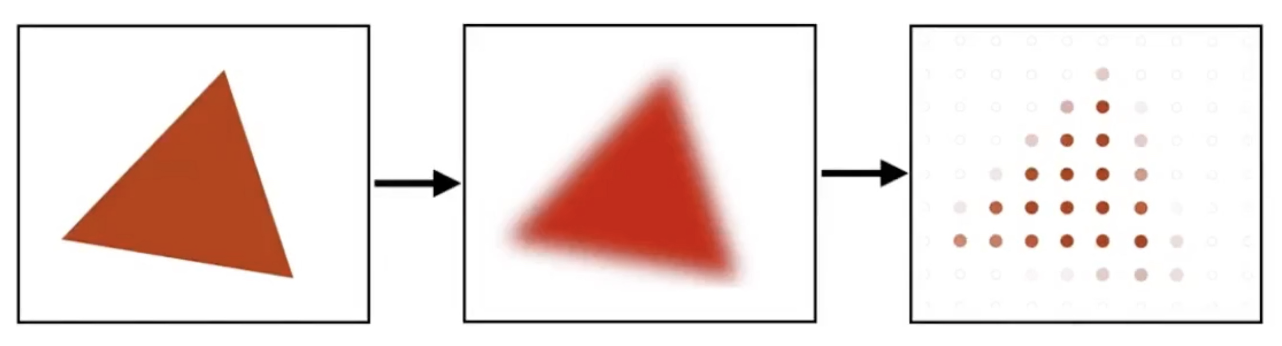
\includegraphics[scale=.3]{antialias.png}
	\caption{反走样过程示意}
	\label{fig:antialias}
\end{figure}

\section{走样产生的原因}
\subsection{傅立叶变换}
任何一个信号都可以表示为一些正弦波和余弦波以及常数的线性表示,我们称之为\textbf{傅立叶展开}。而\textbf{傅立叶变换}指的是将一个时域上的信号转换到频域的过程。
\subsection{走样和滤波}
走样更为学术的定义应该是两个不同频率的信号在使用相同采样的方法后产生的结果无法进行区分。
\begin{figure}[H]
	\centering
	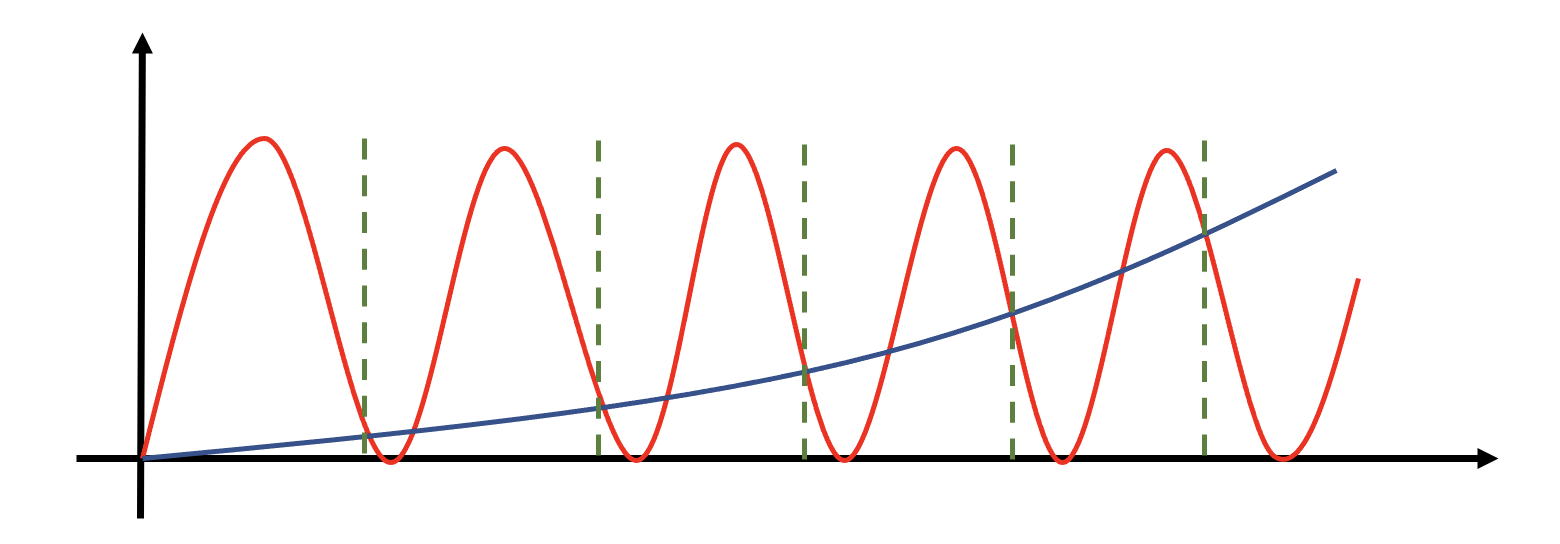
\includegraphics[scale=.3]{caiyang.png}
	\caption{走样示意图}
	\label{fig:alias}
\end{figure}
图中的红色信号和蓝色信号是两个频率不一样的信号,绿色虚线处是采样点,我们发现两个不同频率的信号在同一个采样方式下结果相同,这就产生了走样。

\textbf{滤波(Filter)}是把特定频率的波过滤掉。如果仅保留高频信息,那么这称为高通滤波;如果仅保留低频信息称为低通滤波;如果既删除高频信息,还删除低频信息,只保留中频信息称为带通滤波。

\begin{figure}[H]
	\centering
	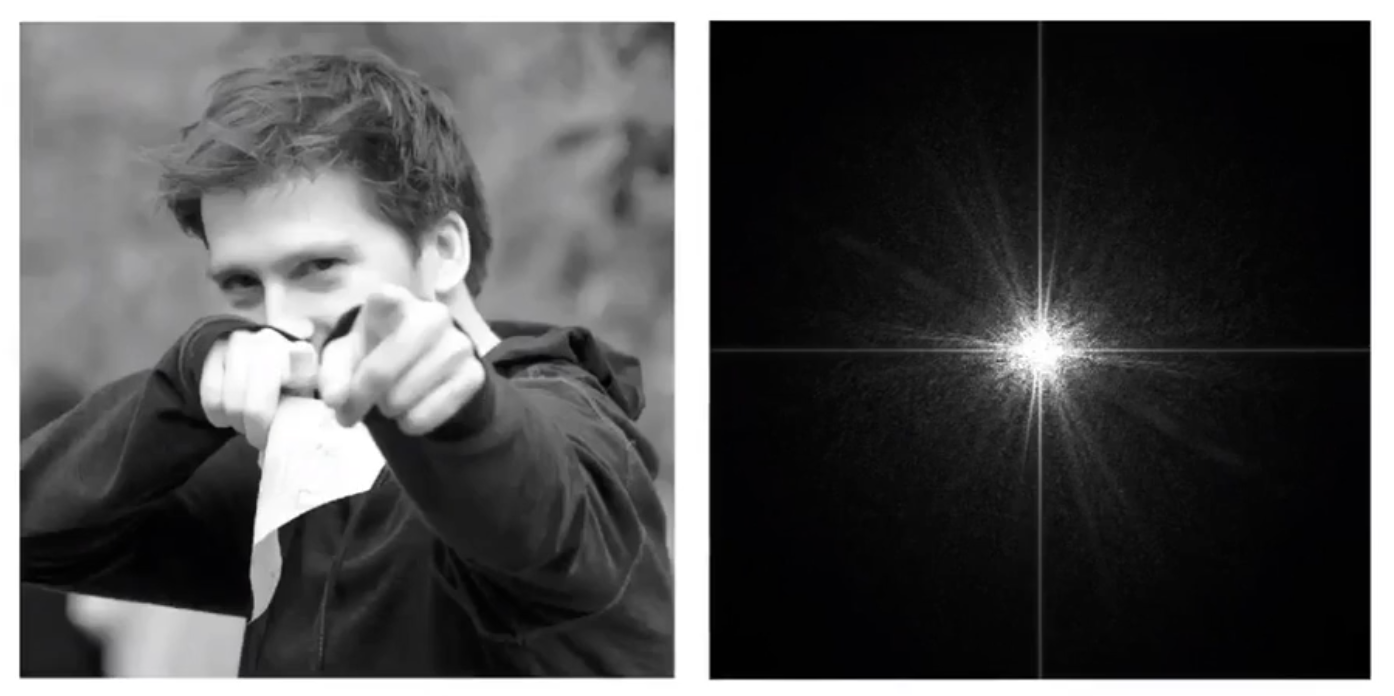
\includegraphics[scale=.3]{fuliye.png}
	\caption{傅立叶变换示意图}
	\label{fig:fuliye}
\end{figure}
对于一个图片我们进行傅立叶变换后,得到的是上面右图的样子。我们进行解释:中心代表了低频信息,边缘代表了高频信息,亮度代表对应频率的能量。对于图片而言,一般低频信息更加的丰富,而高频信息比较少。高频信息一般代表\textbf{边缘信息},因为边缘信息频率比较高;低频信息是图片\textbf{模糊后的结果},频率变化小。
\begin{question}
\textbf{为什么傅立叶变换后图片有一束明显的十字交叉?}

傅立叶变换中我们会认为图片是“连续”的。我们会在原图上下左右不断重复图片以达到“连续”的效果。而图片的四周一般变换非常的快,属于高频的信息,对应在频谱图上就是会有一束明显的十字交叉,代表了高频的边缘信息。
\end{question}

\section{卷积和卷积定律}
滤波可以看作卷积操作,也可以看作平均操作。\textbf{卷积(Convolution)}操作是用一个卷积核在信号上不断地滑动,每一次卷积操作的结果是卷积核和对应位置信号乘积的和,可以看作一次加权平均的过程。

\begin{titledbox}{卷积定律}
	\centering 时域上的卷积等于频域上的乘积,频域上的乘积等于等于频域上的卷积。
\end{titledbox}

\subsection{Box Filter}
\textbf{Box Filter}是一个格式如下的滤波器:
\begin{equation}
	\frac{1}{n^2} X^{n\times n}
\end{equation}
其中,$X$是一个全1矩阵。这个卷积核对临近的$n\times n$的像素做平均。$n$越大,滤波器得到的频率范围越低。

\subsection{深入了解采样}
采样我们可以认为是一个连续函数乘以一系列的脉冲函数的结果。根据卷积定律我们知道,这相当于连续函数的傅立叶变换和脉冲函数傅立叶变换的卷积。脉冲函数的傅立叶变换还是脉冲函数。卷积的结果是信号的频谱在不断地重复。

\begin{figure}[H]
	\centering
	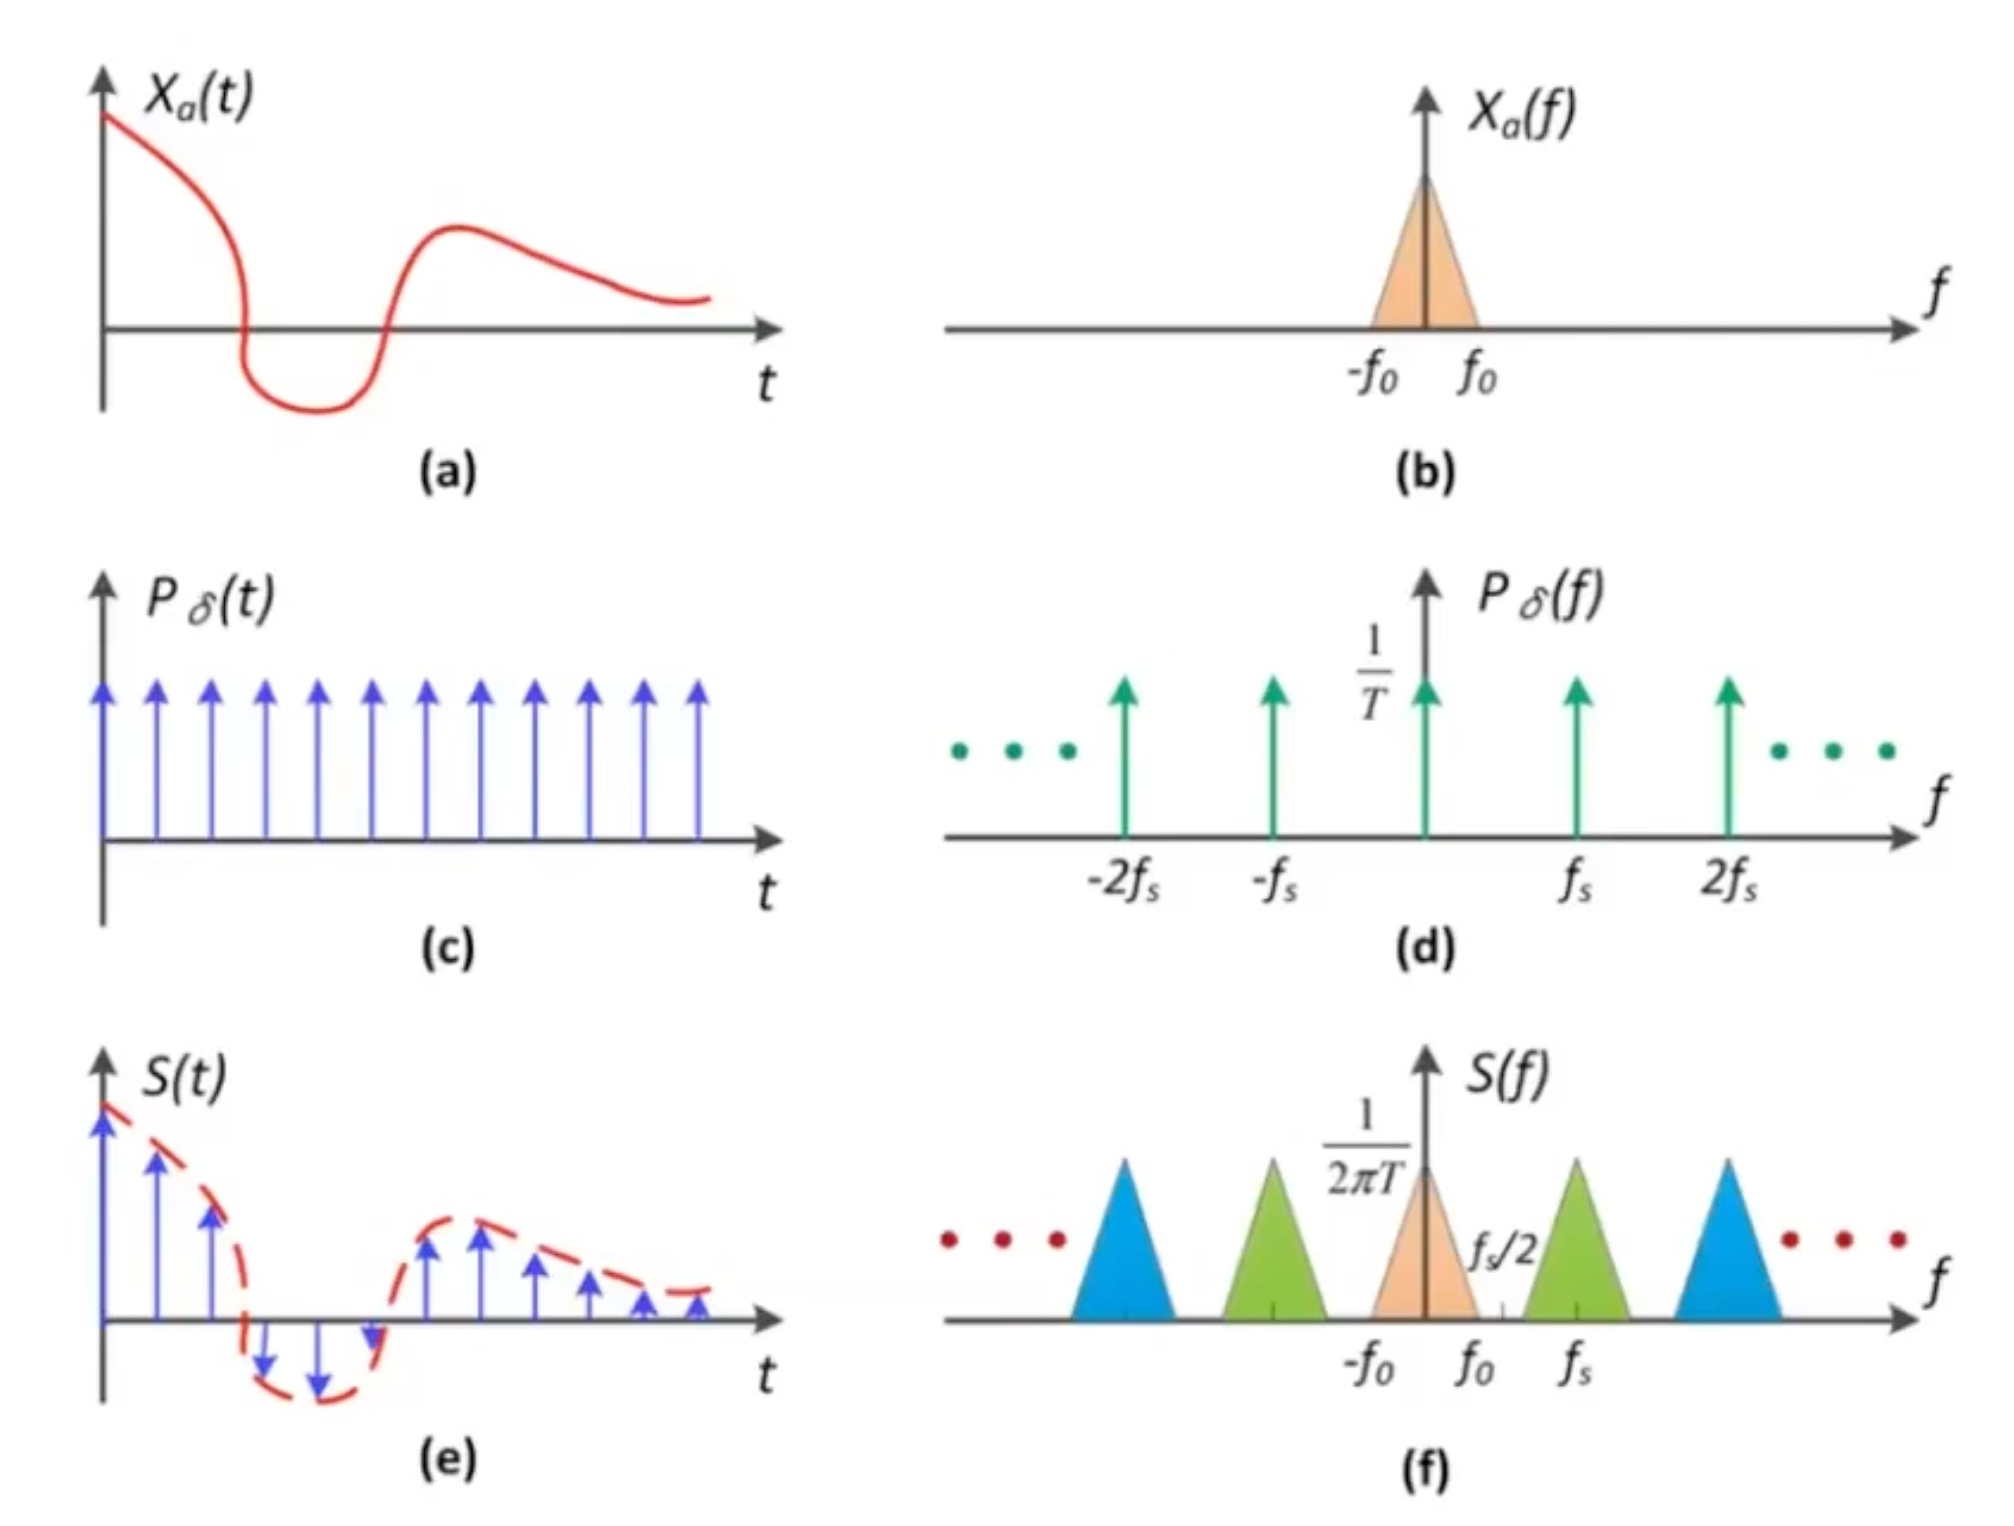
\includegraphics[scale=.15]{caiyang1.png}
	\caption{采样示意图}
	\label{fig:caiyang}
\end{figure}
当采样率不足时会使得频谱之间的间隔太小,导致频谱间产生重叠,这些重叠就是走样。

\begin{figure}[H]
	\centering
	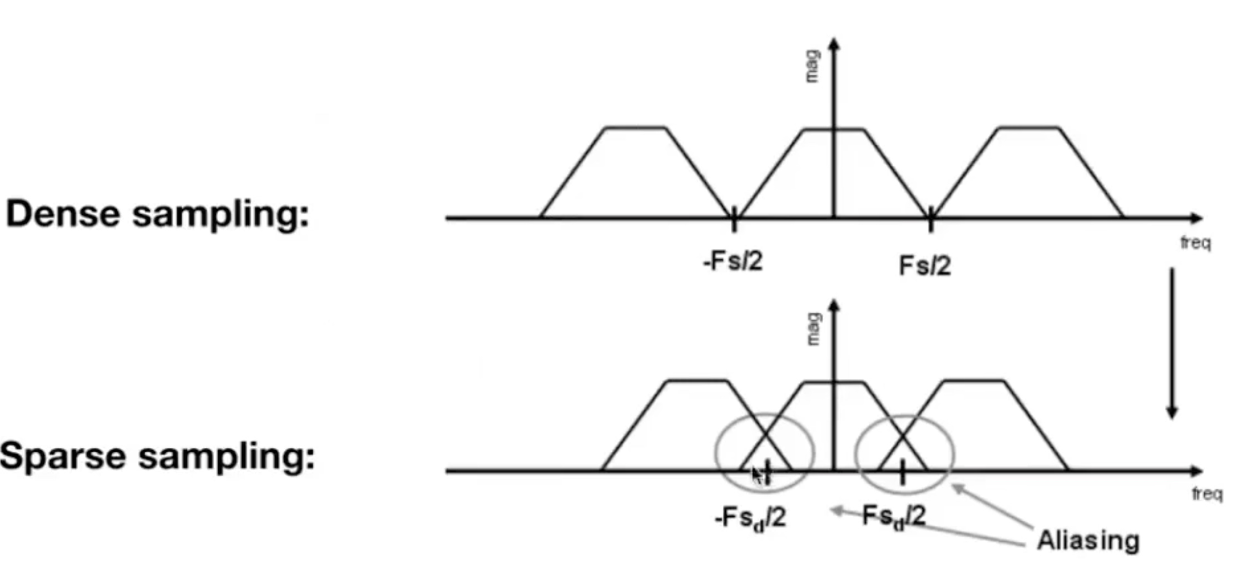
\includegraphics[scale=.4]{pinpuzouyang.png}
	\caption{频谱重叠示意图}
	\label{fig:pinpuzouyang}
\end{figure}

这也就解释了为什么使用高通滤波器可以帮助我们减少走样。这是因为使用高通滤波器只保留更窄的频率范围,可以减少频谱的重叠。

\section{反走样的方法}
目前常用的反走样方法有两种:
\begin{itemize}
	\item 提高采样率(分辨率)。这是从物理层面上提高采样率来减少走样的方式,但是不够实用;
	\item 先进行模糊操作,再进行采样的操作,也就是我们之前所介绍的反走样方法。
\end{itemize}
在实际的操作中,我们使用MSAA(Multi-Sampling Antialiasing)的方式来近似进行反走样的操作,具体的步骤如下:
\begin{enumerate}
	\item 把每一个像素点拆分成$n\times n$的小像素点;
	\item 对每一个小像素点判断该点是否在图形中;
	\item 每一个像素点的结果都是这些小像素点的平均结果。
\end{enumerate}
MSAA仅仅指的是模糊的过程,并不包含采样的过程。这样的方法虽然简单,效果好,但是会增加计算量。在工业界中,一般会采用更为有效的方式拆分采样点,甚至会复用采样点以达到更好的效果。

除此之外,目前业界还有一些其他的方式进行反走样:
\begin{itemize}
	\item FXAA(Fast approximate AA)是通过后期处理的方式处理锯齿。先得到已经有锯齿的图像,找到边界后替换成没有锯齿的边界;
	\item TAA(Temporal AA)是通过抖动的方式进行多次采样,将多个帧合成就相当于多次采样。
\end{itemize}

\section{超分辨率*}
\textbf{超分辨率(Super Sampling)}指的是将一个分辨率较小的图片还原成分辨率较大的图片。和反走样虽然意义不同,但是任务类似。对于超分辨率问题,最重要的是猜测缺失像素的内容,比较适合使用神经网络DLSS(Deep-learning Super Sampling)进行预测。

\section{可见性与遮挡性}
当我们有多个在不同位置的三角形需要进行光栅化的时候,我们需要知道直接三角形的前后关系保证在后面的会被前面的图形遮挡。因此我们需要一定的算法保证前面的图形可以遮挡后面的图形。

\subsection{画家算法}
\textbf{画家算法(Painter's Algorithm)}指的是使用油画的方式进行渲染。我们先光栅化比较远图形,然后光栅化前面的图形进行覆盖。使用这个算法我们需要先对所有的三角形按照远近排序,然后从远到近进行光栅化。对三角形远近的排序的时间复杂度为$O(n\log n)$.这种方法有以下几个问题:
\begin{itemize}
	\item 算法复杂度比较高,并且有时候不好确定各个三角形的远近;
	\item 如果出现互相遮挡的情况形成了一个环,那么采用画家算法失效。
	\begin{figure}[H]
		\centering
		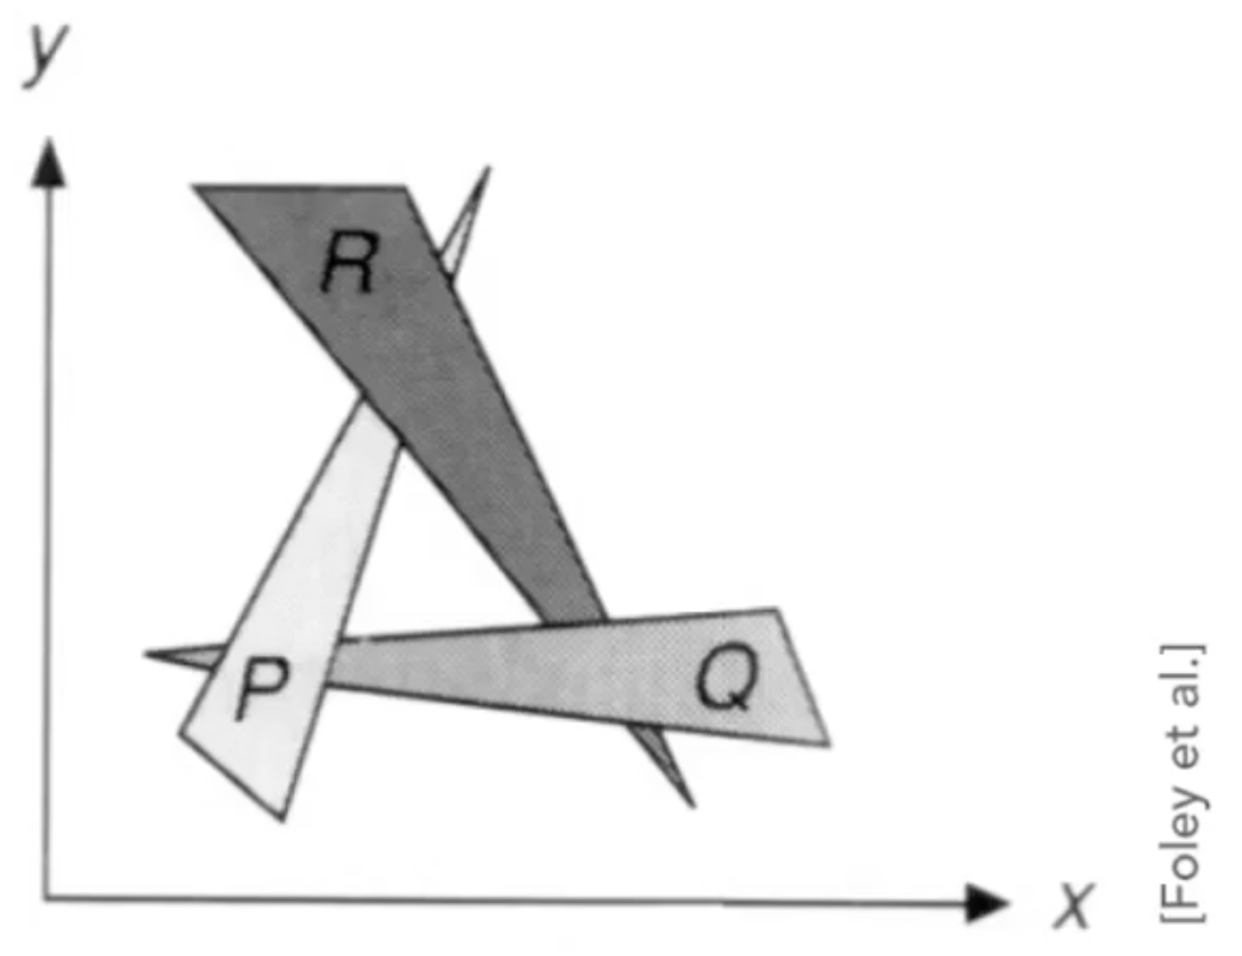
\includegraphics[scale=.2]{huajiasuanfa.png}
		\caption{遮挡成环的情况}
		\label{fig:zhedang}
	\end{figure}
	
\end{itemize}

\subsection{Z Buffer}
我们引入了\textbf{深度缓存技术(Z Bufferi)},记录每一个像素总最近的距离。会生成深度缓存(Depth buffer)和颜色缓存(Frame buffer)。对于任何一个像素,我们通过遍历所有三角形上包含了这点的点选择最近的点保存深度信息和颜色信息。
Z Buffer的算法如下:
\begin{lstlisting}
for(each triangle T)
	for(each sample (x,y,z) in T)
		if(z < zbuffer[x,y])
			framebuffer[x,y] = rgb;
			zbuffer[x,y] = z;
		else
			;        //什么也不做
\end{lstlisting}
深度缓存技术的时间复杂度是$O(n)$。这并不是一个排序算法,因此复杂度比排序算法要小。如果MASS中需要深度缓存技术,需要对每一个采样点使用Z Buffer算法。

\part{着色}

\chapter{Blinn-Phong反射模型}
在计算机图形学中,着色指的是对于不同的物体应用不同的材质。我们知道,光的反射我们需要进行进行建模。一个简单的光学模型就是\textbf{Blinn-Phong反射模型(Blinn-Phong Reflection Model)}。基本的模型一般会有以下几个部分:漫反射,高光(镜面反射),环境光(在这里我们不考虑环境光反射,我们认为这是一个常量)。

\section{模型定义}
\begin{figure}[H]
	\centering
	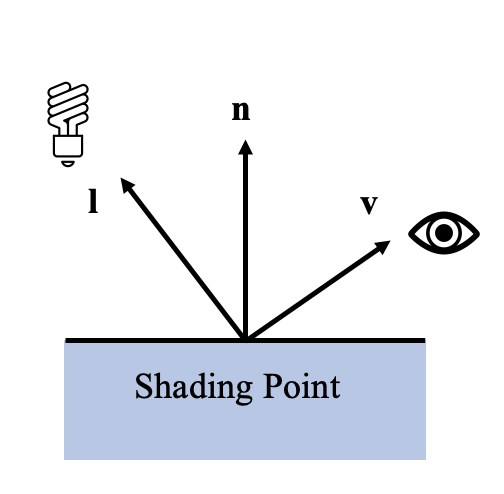
\includegraphics[scale=.6]{fanshemoxing.png}
	\caption{光线反射模型}
	\label{fig:fanshe}
\end{figure}
对于任何的着色点,我们定义了:
\begin{itemize}
	\item 法线$\overrightarrow{n}$,是垂直于反射面的线;
	\item 观察方向$\overrightarrow{v}$,是着色点和观察点的连线;
	\item 光照方向$\overrightarrow{l}$,是着色点和光源的连线。
\end{itemize}
以上的方向向量都是单位向量。同时我们还需要定义物体表面的参数,例如颜色,亮度。当我们着色时,我们不考虑其他的物体遮挡,因此着色中没有阴影。

\section{漫反射}
漫反射指的是一束光线会向各个方向均匀地反射。

\subsection{Lambert's 余弦定律}
\textbf{Lambert's 余弦定律(Lambert's Cosine Law)}说明了漫反射光的能量和入射角度之间的关系。光线反射的能量和光照方向和发现的夹角cos值(向量点乘的结果)成正比关系。

\subsection{点光源}
我们认为光源是一个点。在同一时刻光的能量集中在同一个球壳上。根据能量守恒定律我们可以得知,每一个球壳上光能量相同。随着球壳变大,单位面积上的光能量减小。我们定义距离为1的光能量为$I$。光能量和距离成平方反比关系,距离为$r$的地方的光能量为$\frac{I}{r^2}$.

\subsection{漫反射计算公式}
漫反射能量的计算公式如下:
\begin{equation}
	L_d = k_d\ \frac{I}{r^2}\ \text{max}(0, \textbf{n\cdot l})
\end{equation}
这里,$k_d$代表吸收率,如果用RGB定义一个向量作为吸收率就可以代表这个反射点的颜色。$\text{max}(0, \textbf{n\cdot l})$可以把反射光线在反方向的光线过滤掉,这些光线没有贡献。同时,漫发射和观察的方向无关

\section{高光(镜面反射)}
我们认为光滑的平面可以满足基本的镜面反射的物理规律(入射角等于反射角)。当我们的观察方向和反射角方向一直的时候就可以看到高光。我们一般使用半程向量和法线的接近程度来“映射”观察方向和反射角的接近程度。半程向量指的是光源方向和观察方向角平分线上的方向向量。
\begin{equation}
	\textbf{h} = \text{bisector}(\textbf{v}, \textbf{l}) = \frac{\textbf{v} + \textbf{l}}{||\textbf{v} + \textbf{l}||}
\end{equation}
高光的计算公式如下:
\begin{equation}
	L_s = k_s\ \frac{I}{r^2}\ \text{max}(0, \textbf{n\cdot h})^p
\end{equation}
一边来说高光的颜色$k_s$为白色。我们会给cos项乘一个指数$p$。原因是余弦函数的容忍度很高,但是我们希望当角度偏离一点点的时候就看不到高光。因此会使用一个指数,一般来说$p\in [100,200]$。
\begin{figure}[H]
	\centering
	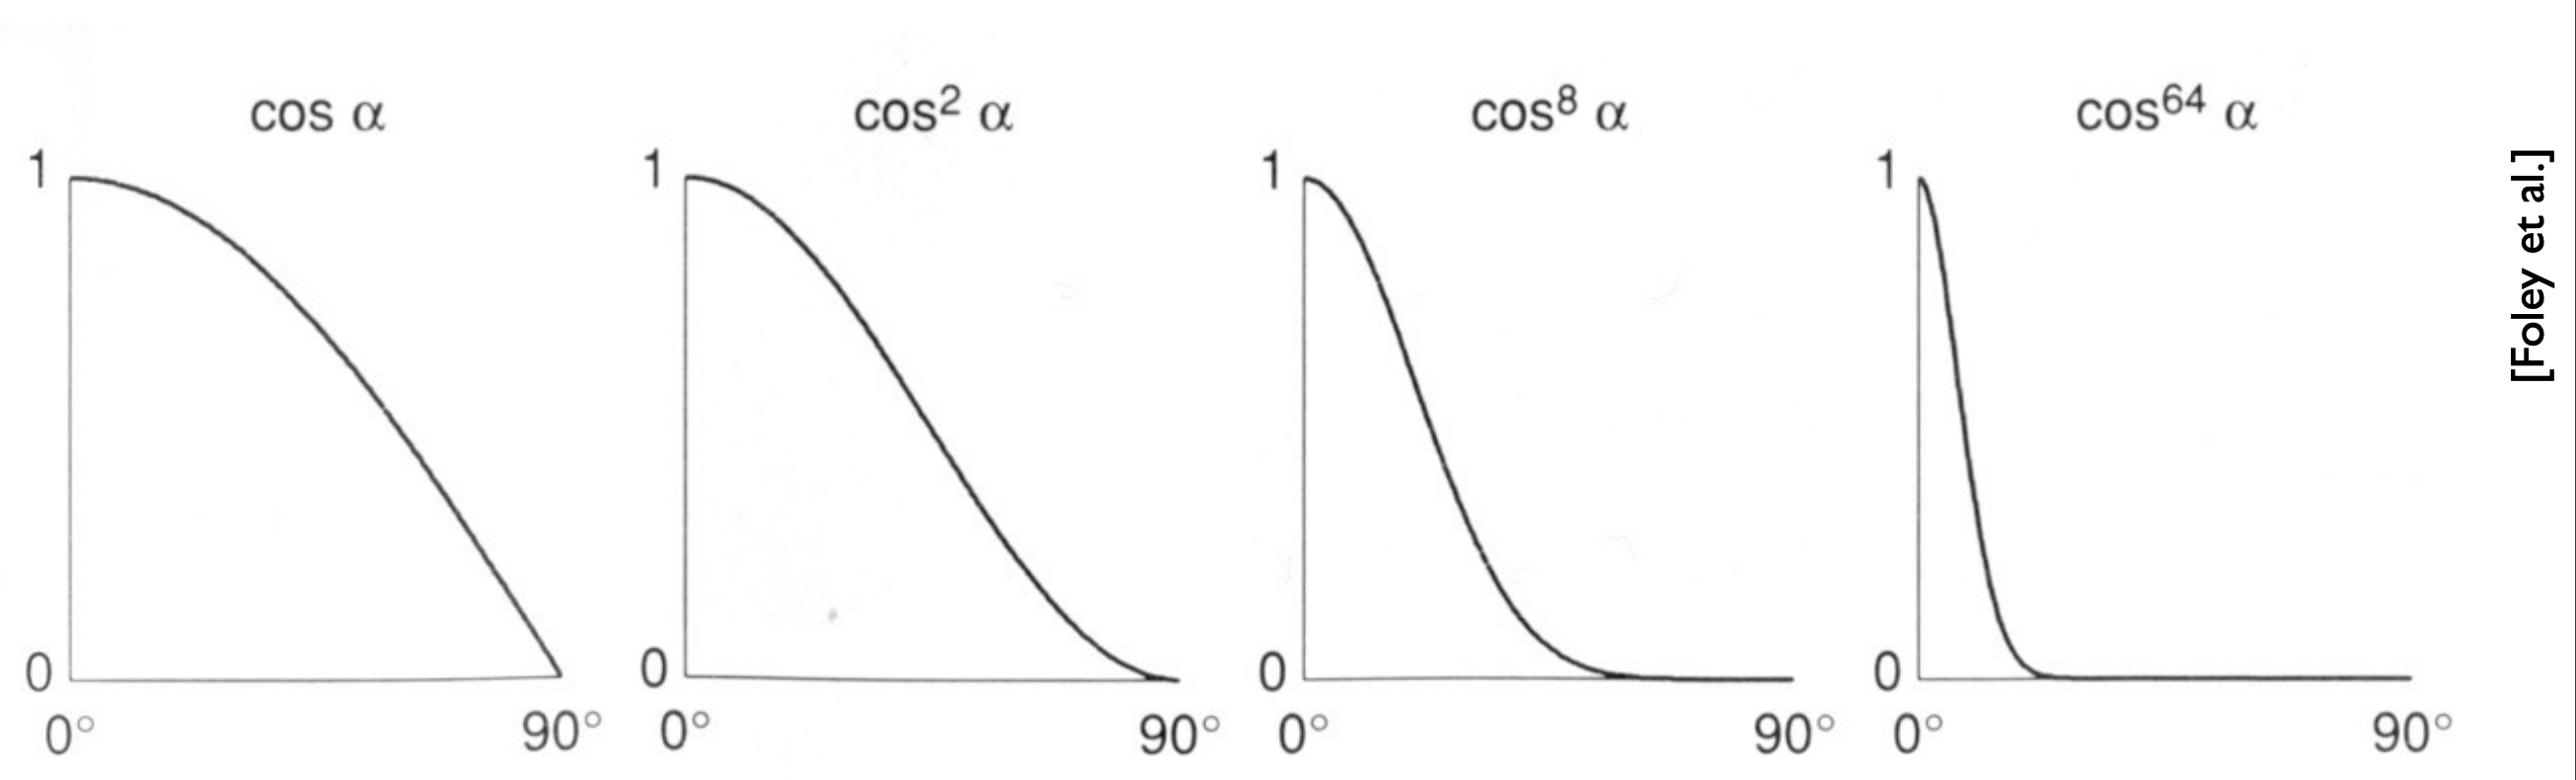
\includegraphics[scale=.2]{cos.png}
	\caption{指数的选择}
	\label{fig:cos}
\end{figure}

\section{环境光照}
我们粗略的认为环境中所有点的光照相同,是一个常数。环境光与光源方向,法线方向和观察方向无关。计算公式如下:
\begin{equation}
	L_a = k_a\ I_a
\end{equation}

\section{Blinn-Phong反射模型}
综上所述,Blinn-Phong反射模型可以表示为:
\begin{equation}
	L = L_a + L_d + L_s = k_a\ I_a +  k_d\ \frac{I}{r^2}\ \text{max}(0, \textbf{n\cdot l}) + k_s\ \frac{I}{r^2}\ \text{max}(0, \textbf{n\cdot h})^p
\end{equation}
\begin{figure}[H]
	\centering
	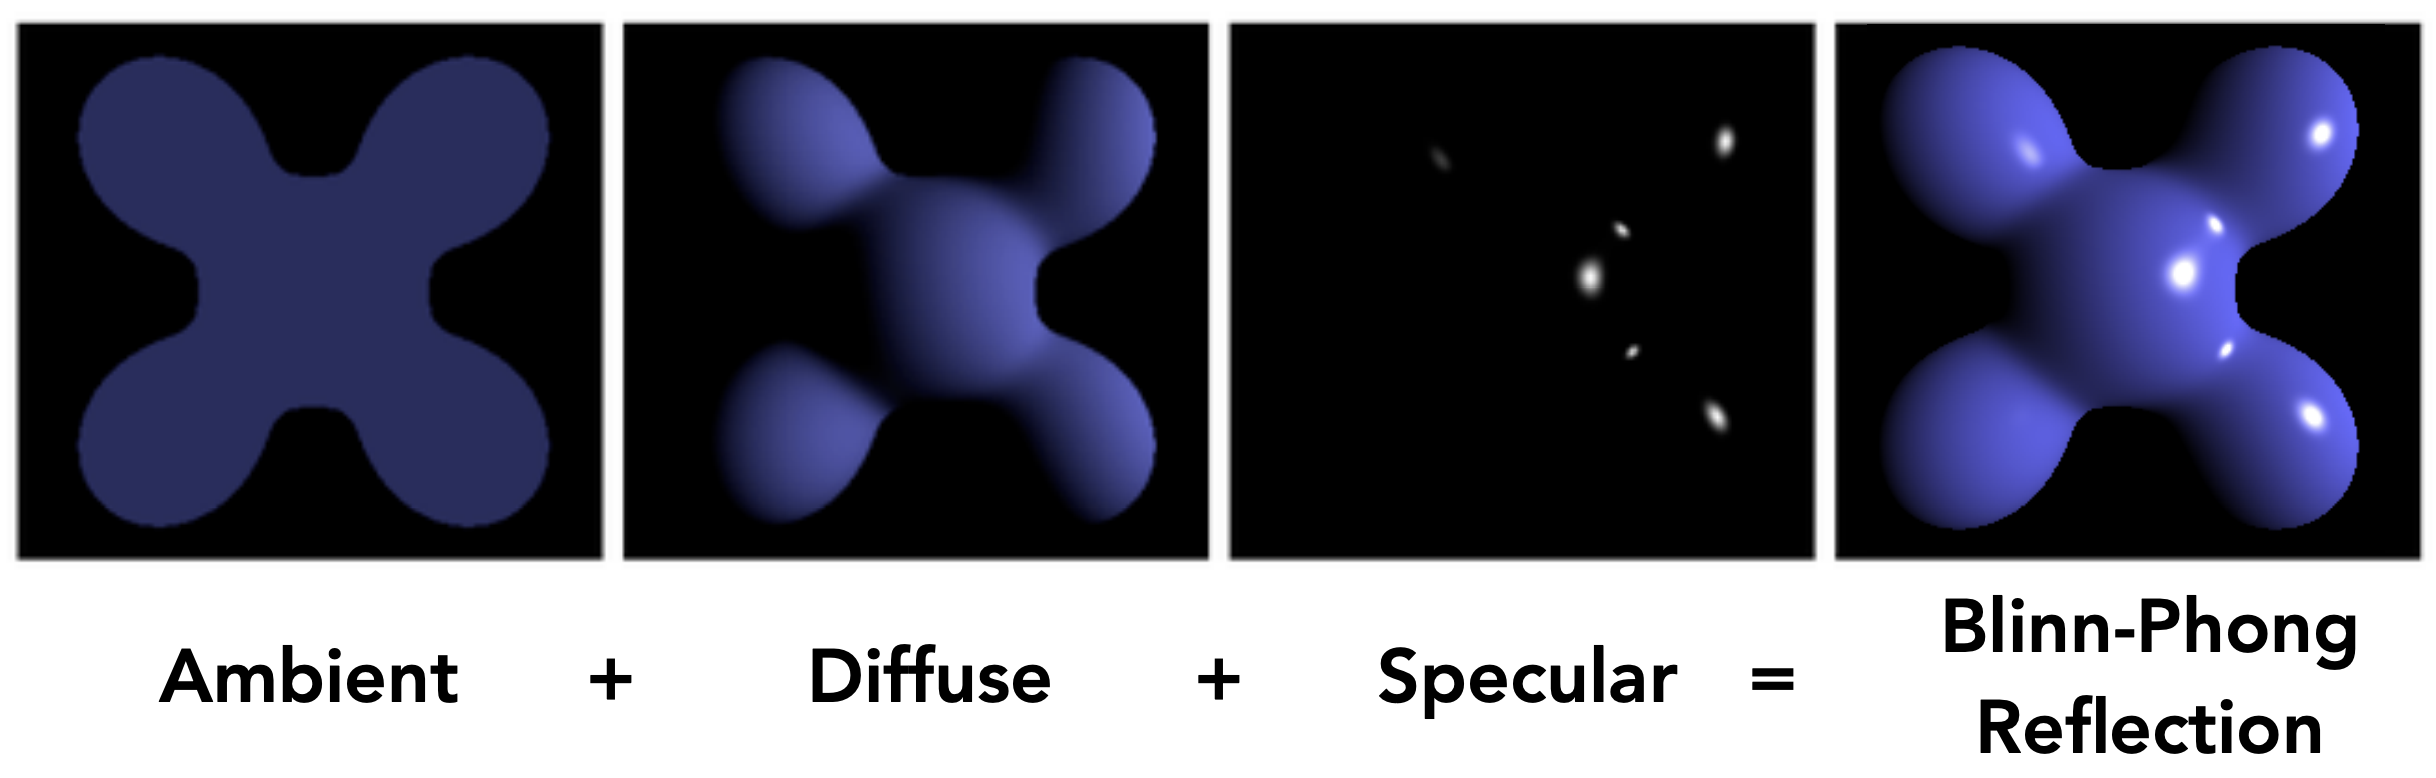
\includegraphics[scale=.3]{phonemodel.png}
	\caption{Blinn-Phong反射模型}
	\label{fig:phonemodel}
\end{figure}

\chapter{着色频率和管线}

\section{着色频率}
根据不同的着色方式,有不同的着色频率,主要的着色频率分为三种——面着色,顶点着色和像素着色。主要的不同之处在于法线的选择方式不同。

\begin{itemize}
	\item \textbf{面着色(Flat Shading)}指的是计算每一个三角形平面的法线后对一个平面整体进行着色;
	\item \textbf{顶点着色(Gouraud Shading)}指的是计算每一个三角形三个顶点的法线后进行着色,最后在三角形内部插值得到颜色。顶点法线的计算是通过顶点相邻面的法线的(加权)平均值求出;
	\item \textbf{像素着色(Phong Shading)}指的是计算出每一个像素的法线进行着色。三角形内部点法线的计算需要依靠重心坐标计算。
\end{itemize}
当几何体相对复杂,构造精细的时候,三种着色效果产生的结果不相上下。

\section{(实时渲染)管线}
\textbf{管线(Pipeline)}是从模型到图片生成的过程。管线分为以下过程:
\begin{figure}[H]
	\centering
	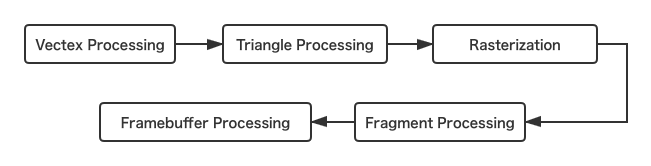
\includegraphics[scale=.6]{pipeline.png}
	\caption{管线}
	\label{fig:pipeline}
\end{figure}

首先将顶点的三位向量作为输入,进行几何变换后划分三角形区域。通过光栅化获得一个个小的碎片(或者是一个个小像素)后进行着色,得到我们的输出。

我们可以定义顶点或者像素的着色方式来提供不同的着色要求,这被称为\textbf{Shader}。硬件中会提供这样的编程方式定制不同的着色方式,以OpenGL为例,我们可以定义以下的着色函数:
\begin{lstlisting}
uniform sampler2D myTexture;
uniform vec3 lightDir;
varying vec2 uv;
varying vec3 norm;

void diffuseShader(){
	vec3 kd;
	kd = texture2d(myTexture, uv);
	kd *= clamp(dot(-lightDir, norm), 0.0, 1.0);
	gl_FragColor = (kd, 1.0);
}
\end{lstlisting}
这里我们定义了一个简单的漫反射着色器。同时,着色器会自动应用到每一个顶点或者是像素上,不需要我们使用显式的for循环进行遍历。

\begin{information}
	我们可以进入Shadertoy网站(\url{https://www.shadertoy.com/view/ld3Gz2})练习Shader编程,编程的结果会直接显示在网页中。
\end{information}

\chapter{纹理映射}

对于任何一个三角形,我们在内部填充一个图形作为纹理。\textbf{纹理(Texture)}也就是我们在不同的位置所定义的漫反射系数。

\section{三维物体表面展开}

任何一个三维物体的表面都是二维的图形,我们可以将一个三维物体表面映射到一个二维的图像上。图形的映射非常的复杂,这里不做过多解释。我们将纹理建立一个$u-v$坐标系。同时$u,v\in[0,1]$。

当然,我们在为墙面,地面加入纹理的时候可以使用边缘连接连续的纹理,称为\textbf{tiled}。这样子就可以复用纹理拼接大表面。我们可以知道每一个三角形的顶点坐标和对应的纹理坐标,那么我们怎么求出来三角形内部顶点坐标对应的纹理坐标。这就是一个插值问题,我们需要使用重心坐标的方式计算。

\section{重心坐标}
我们在之前的节中留下了以下疑问,已知三角形三个顶点的颜色,法线或者纹理坐标,如何求出三角形内部某一点对应的插值量?这个时候我们就需要使用\textbf{重心坐标(Barycentric Coordinate)}来计算。

对于$\triangle ABC$内任意一点$(x,y)$可以满足:
\begin{equation}
	\begin{split}
		&(x,y) = \alpha A + \beta B + \gamma C, \\
		&\alpha + \beta + \gamma = 1,\\
		& \alpha, \beta, \gamma >= 0
	\end{split}
\end{equation}
三角形平面上的任意一点都可以用三角形三个顶点坐标的线性组合表示。三角形内部的点必须满足系数加和为1并且系数均为非负数。那么重心坐标就是$(\alpha,\beta,\gamma)$,已知任意两个重心坐标可以直接推断出第三个坐标。
重心坐标可以通过面积求出,我们令三角形内一点和三个顶点相连,每一个顶点所对的小三角形的面积为$A_A,A_B,A_C$,那么重心坐标可以用以下方式计算:
\begin{figure}[H]
	\centering
	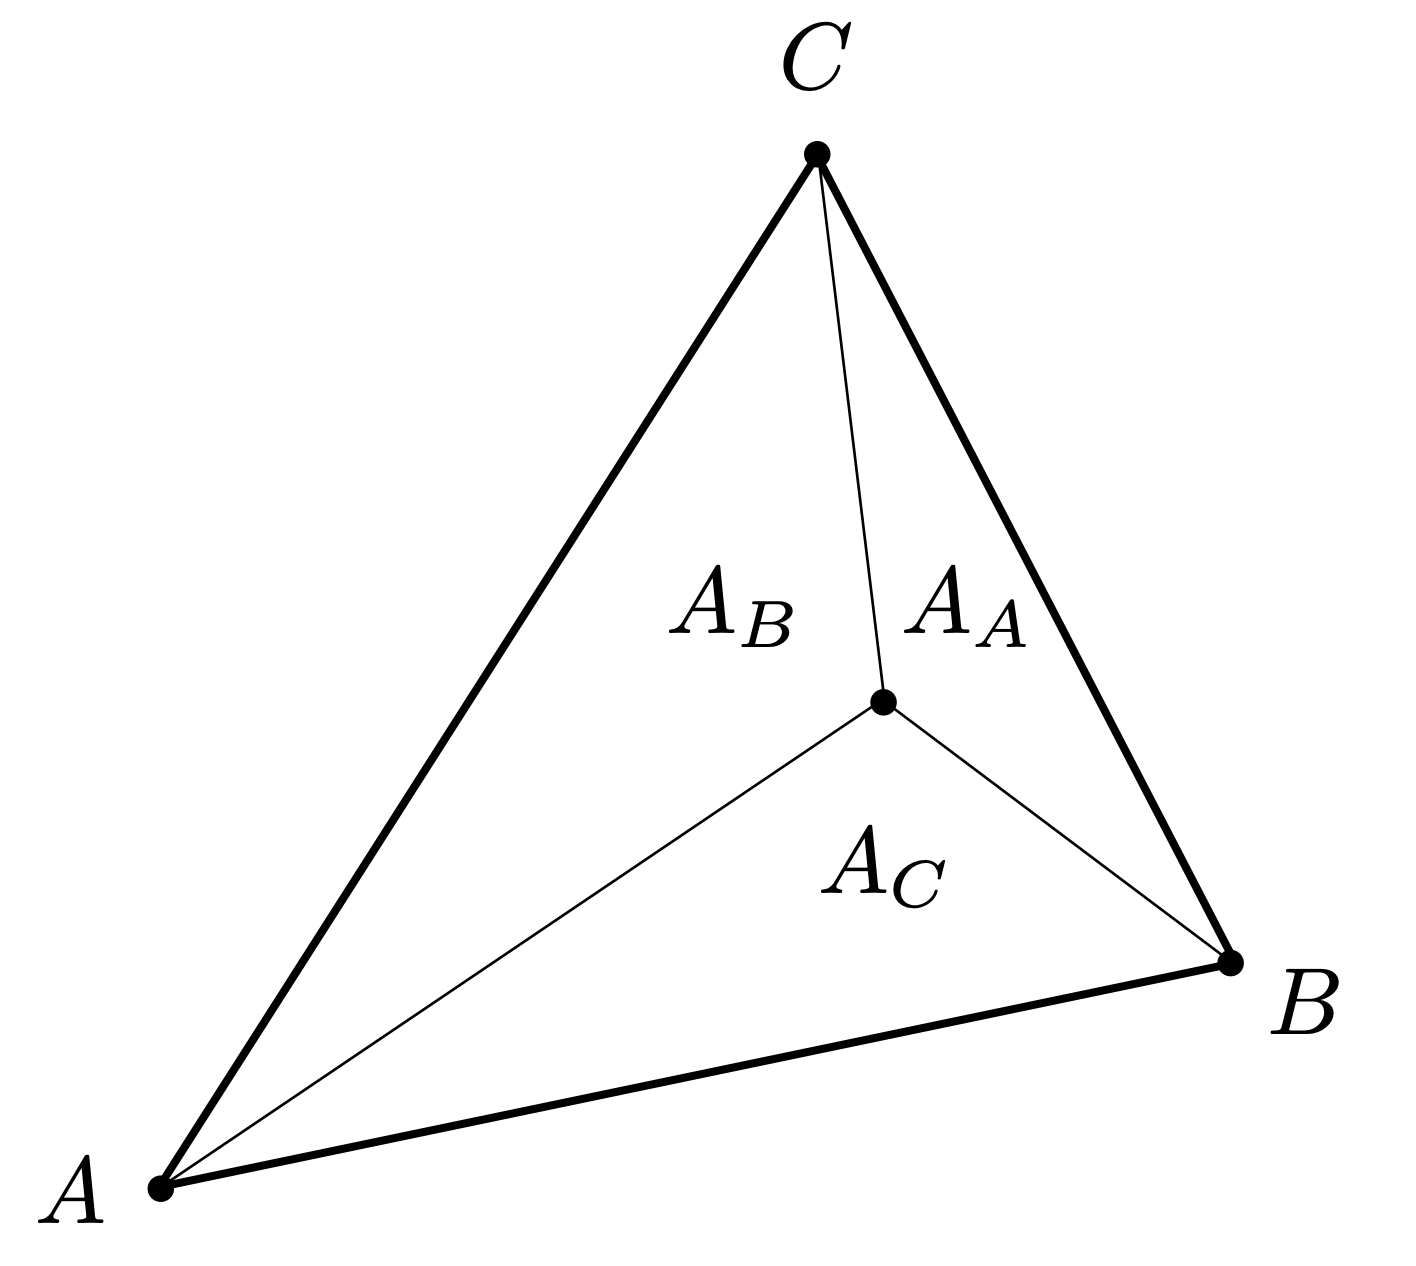
\includegraphics[scale=.15]{zhongxinzuobiao.png}
	\caption{重心坐标的计算}
	\label{fig:zongxinzuobiao}
\end{figure}
\begin{equation}
	\begin{split}
		\alpha = \frac{A_A}{A_A+A_B+A_C},\\
		\beta = \frac{A_B}{A_A+A_B+A_C},\\
		\gamma = \frac{A_C}{A_A+A_B+A_C}\\
	\end{split}
\end{equation}
当重心坐标为$(\frac{1}{3},\frac{1}{3},\frac{1}{3})$的时候,这个点是三角形的重心。已知三个顶点的坐标也可以直接推算出重心坐标:
\begin{equation}
	\begin{split}
		&\alpha = \frac{-(x-x_B)(y_C-y_B) + (y-y_B)(x_C-x_B)}{-(x_A-x_B)(y_C-y_B) + (y_A-y_B)(x_C-x_B)},\\
		&\beta =  \frac{-(x-x_C)(y_A-y_C) + (y-y_C)(x_A-x_C)}{-(x_B-x_C)(y_A-y_C) + (y_B-y_C)(x_A-x_C)},\\
		&\gamma = 1-\alpha-\beta\\
	\end{split}
\end{equation}

如果三角形三个顶点对应了三个向量(颜色,法线或者纹理坐标),那么内部点对应的向量值是使用重心坐标进行的线性组合。假设三个顶点对应的向量是$V_A,V_B,V_C$,那么三角形中任意一点的插值后向量是$V=\alpha V_A +\beta V_B+\gamma V_C$。同时,重心坐标在投影后不能保证结果不变,因此我们在空间中需要使用三维坐标计算的重心坐标来进行插值。

\section{纹理映射的问题}
纹理映射主要分为两步,第一步是把像素点坐标映射到纹理坐标$(x,y)\rightarrow (u,v)$。第二部根据纹理坐标得到对应的漫反射系数$(u,v)\rightarrow k_d$,纹理上的像素叫做纹理元素或者纹素(Texel)。但是如果纹理过大或者过小都会出现一些问题。

\textbf{如果纹理太小的话......}

如果纹理本身太小,但是物体像素点比较多,那么就会产生非常多类似于马赛克的像素。这是由于很多像素点会求出浮点数纹理坐标,在取整后会导致马赛克的产生。我们用两种方式解决,一种是双线性插值法,另一种是二次样条插值法。
\begin{figure}[H]
	\centering
	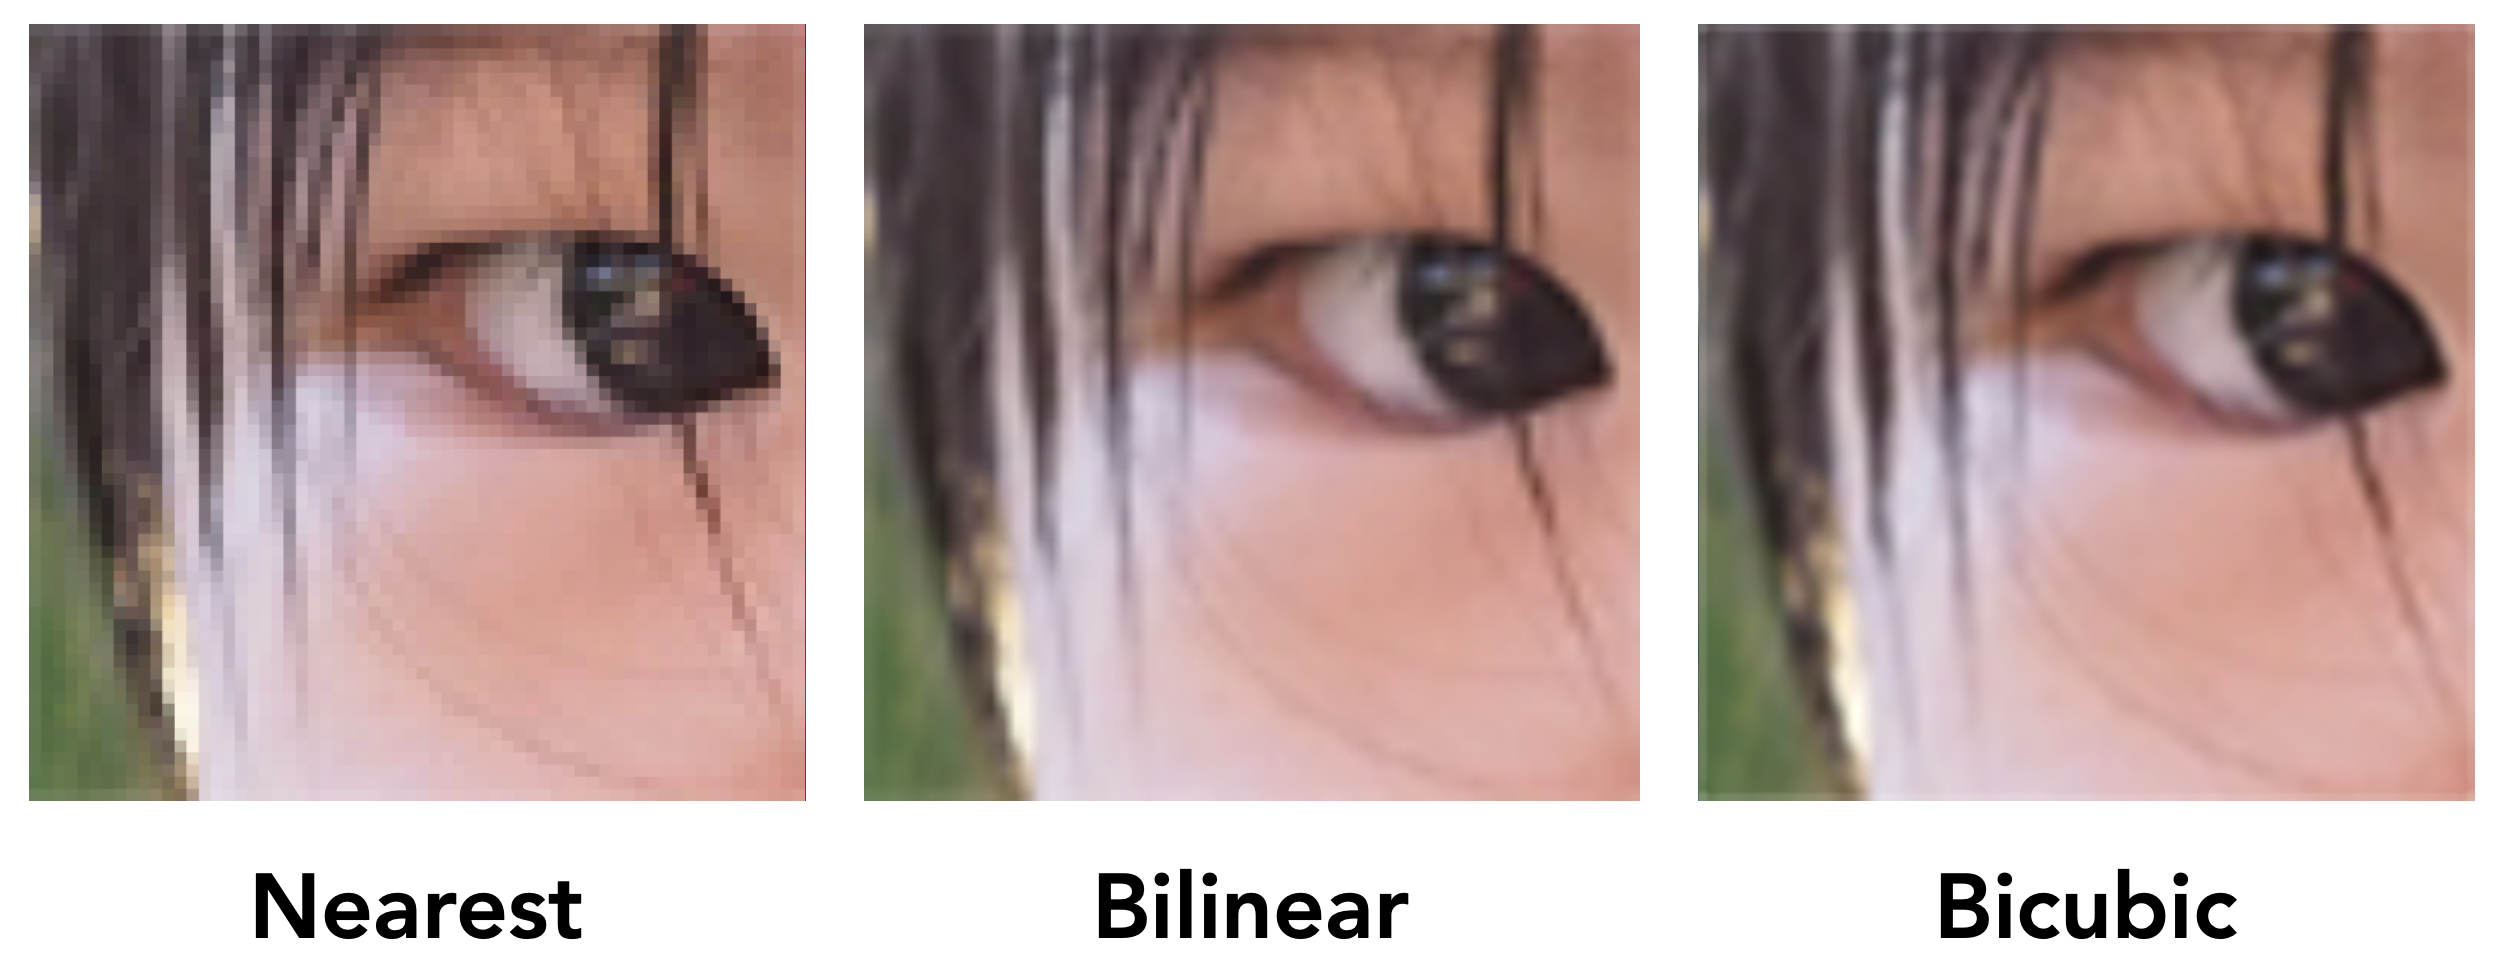
\includegraphics[scale=.25]{chazhi.png}
	\caption{纹理过小的解决方案}
	\label{fig:chazhi}
\end{figure}

\textbf{双线性插值(Bilinear Interpolation)}指的是对于任意一个纹理坐标,我们使用其临近的四个纹素值进行两次线性插值得到这个坐标对应的漫反射率。

\begin{figure}[H]
	\centering
	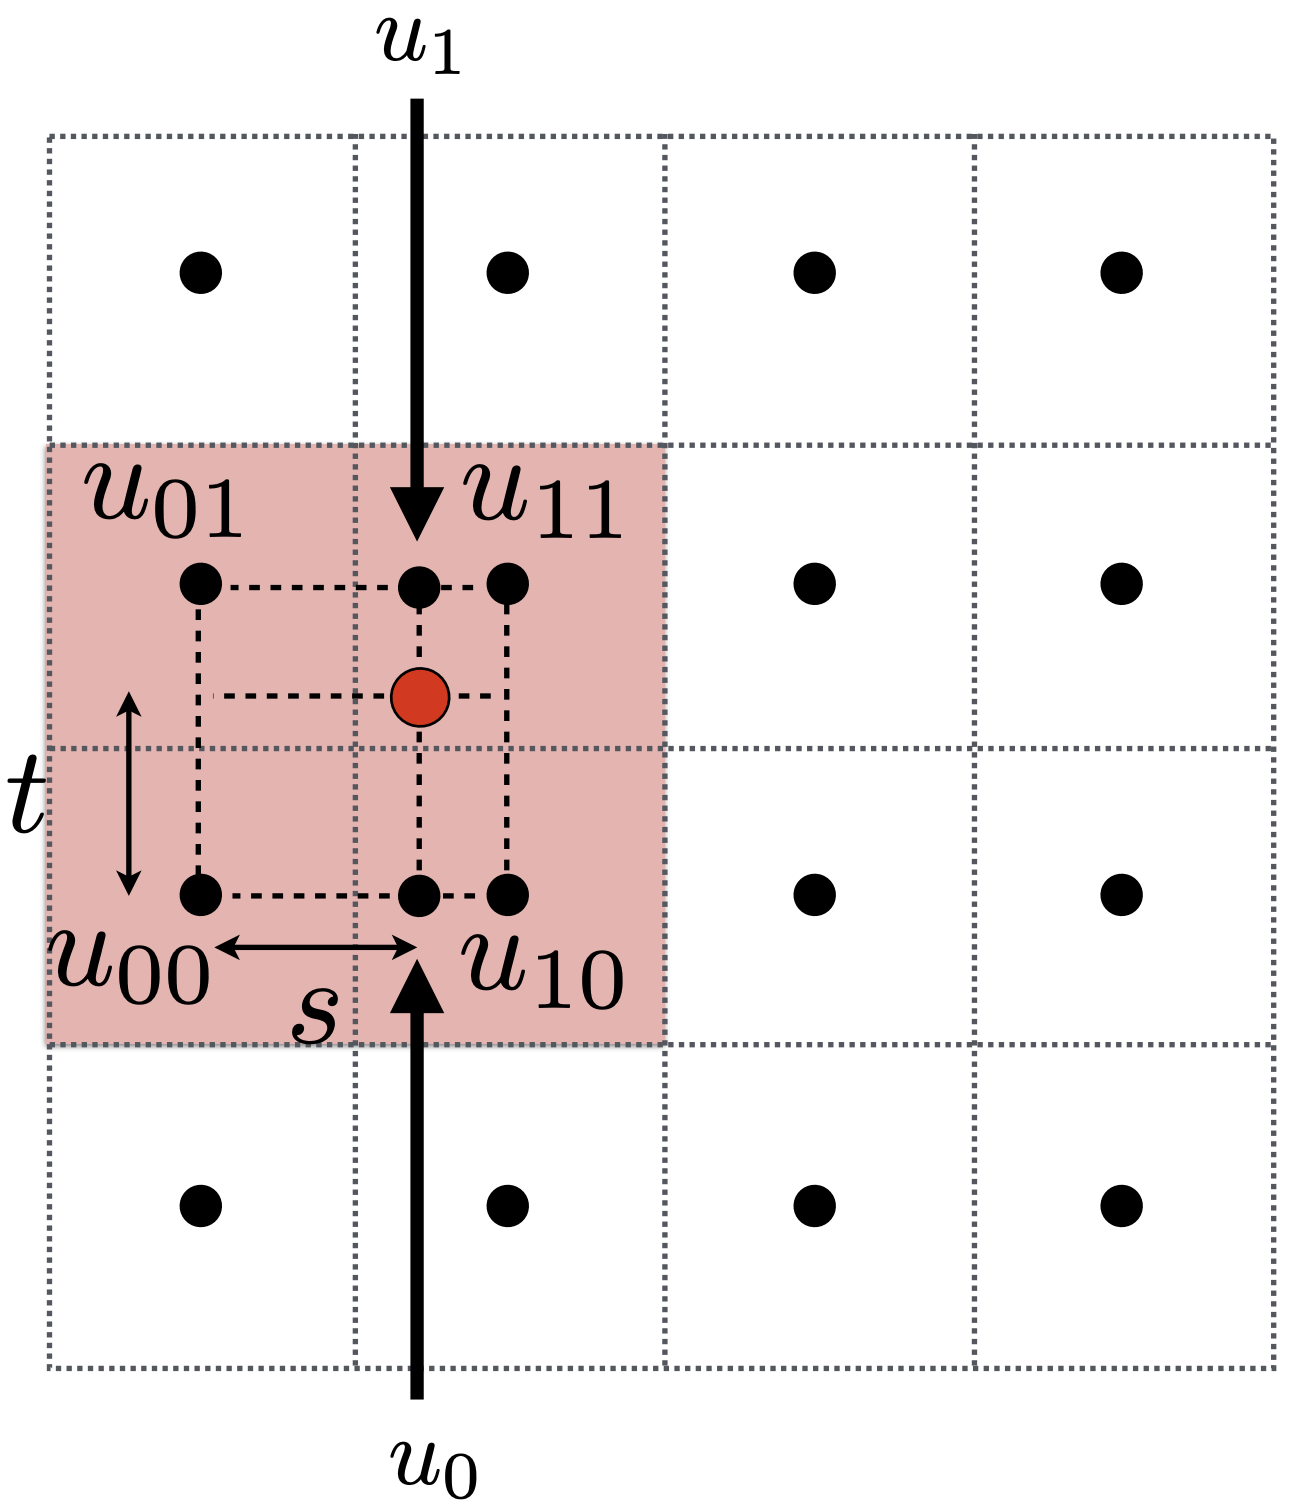
\includegraphics[scale=.15]{shuangxianxing.png}
	\caption{双线性插值示意图}
	\label{fig:shuangxianxing}
\end{figure}
在一维上的线性插值可以表示为:$\text{lerp}(x,v_0,v_1)=v_0+x(v_1-v_0)$。首先我们在水平方向上做两次线性插值:
\begin{equation}
	\begin{split}
		u_0 = \text{lerp}(s,u_{00},u_{10})\\
		u_1 = \text{lerp}(s,u_{01},u_{11})\\
	\end{split}
\end{equation}
然后我们在纵向上做一次线性插值:
\begin{equation}
		f(x,y) = \text{lerp}(s,u_{0},u_{1})\\
\end{equation}
插值的结果相比于之前变化更加顺畅。

\textbf{双立方插值(Bicubic Interpolation)}使用相邻16个点进行计算,效果更好但是计算量相对来说更大。

\textbf{如果纹理太大的话......}

当纹理过大的时候,近处的物体会产生锯齿,远处的物体会产生摩尔纹,也就是说结果会产生走样。主要原因是因为当物体离得越远,每一个像素所代表的纹素的数量会变多。这个时候再使用像素和纹素一一对应的方式是不可靠的。
\begin{figure}[H]
	\centering
	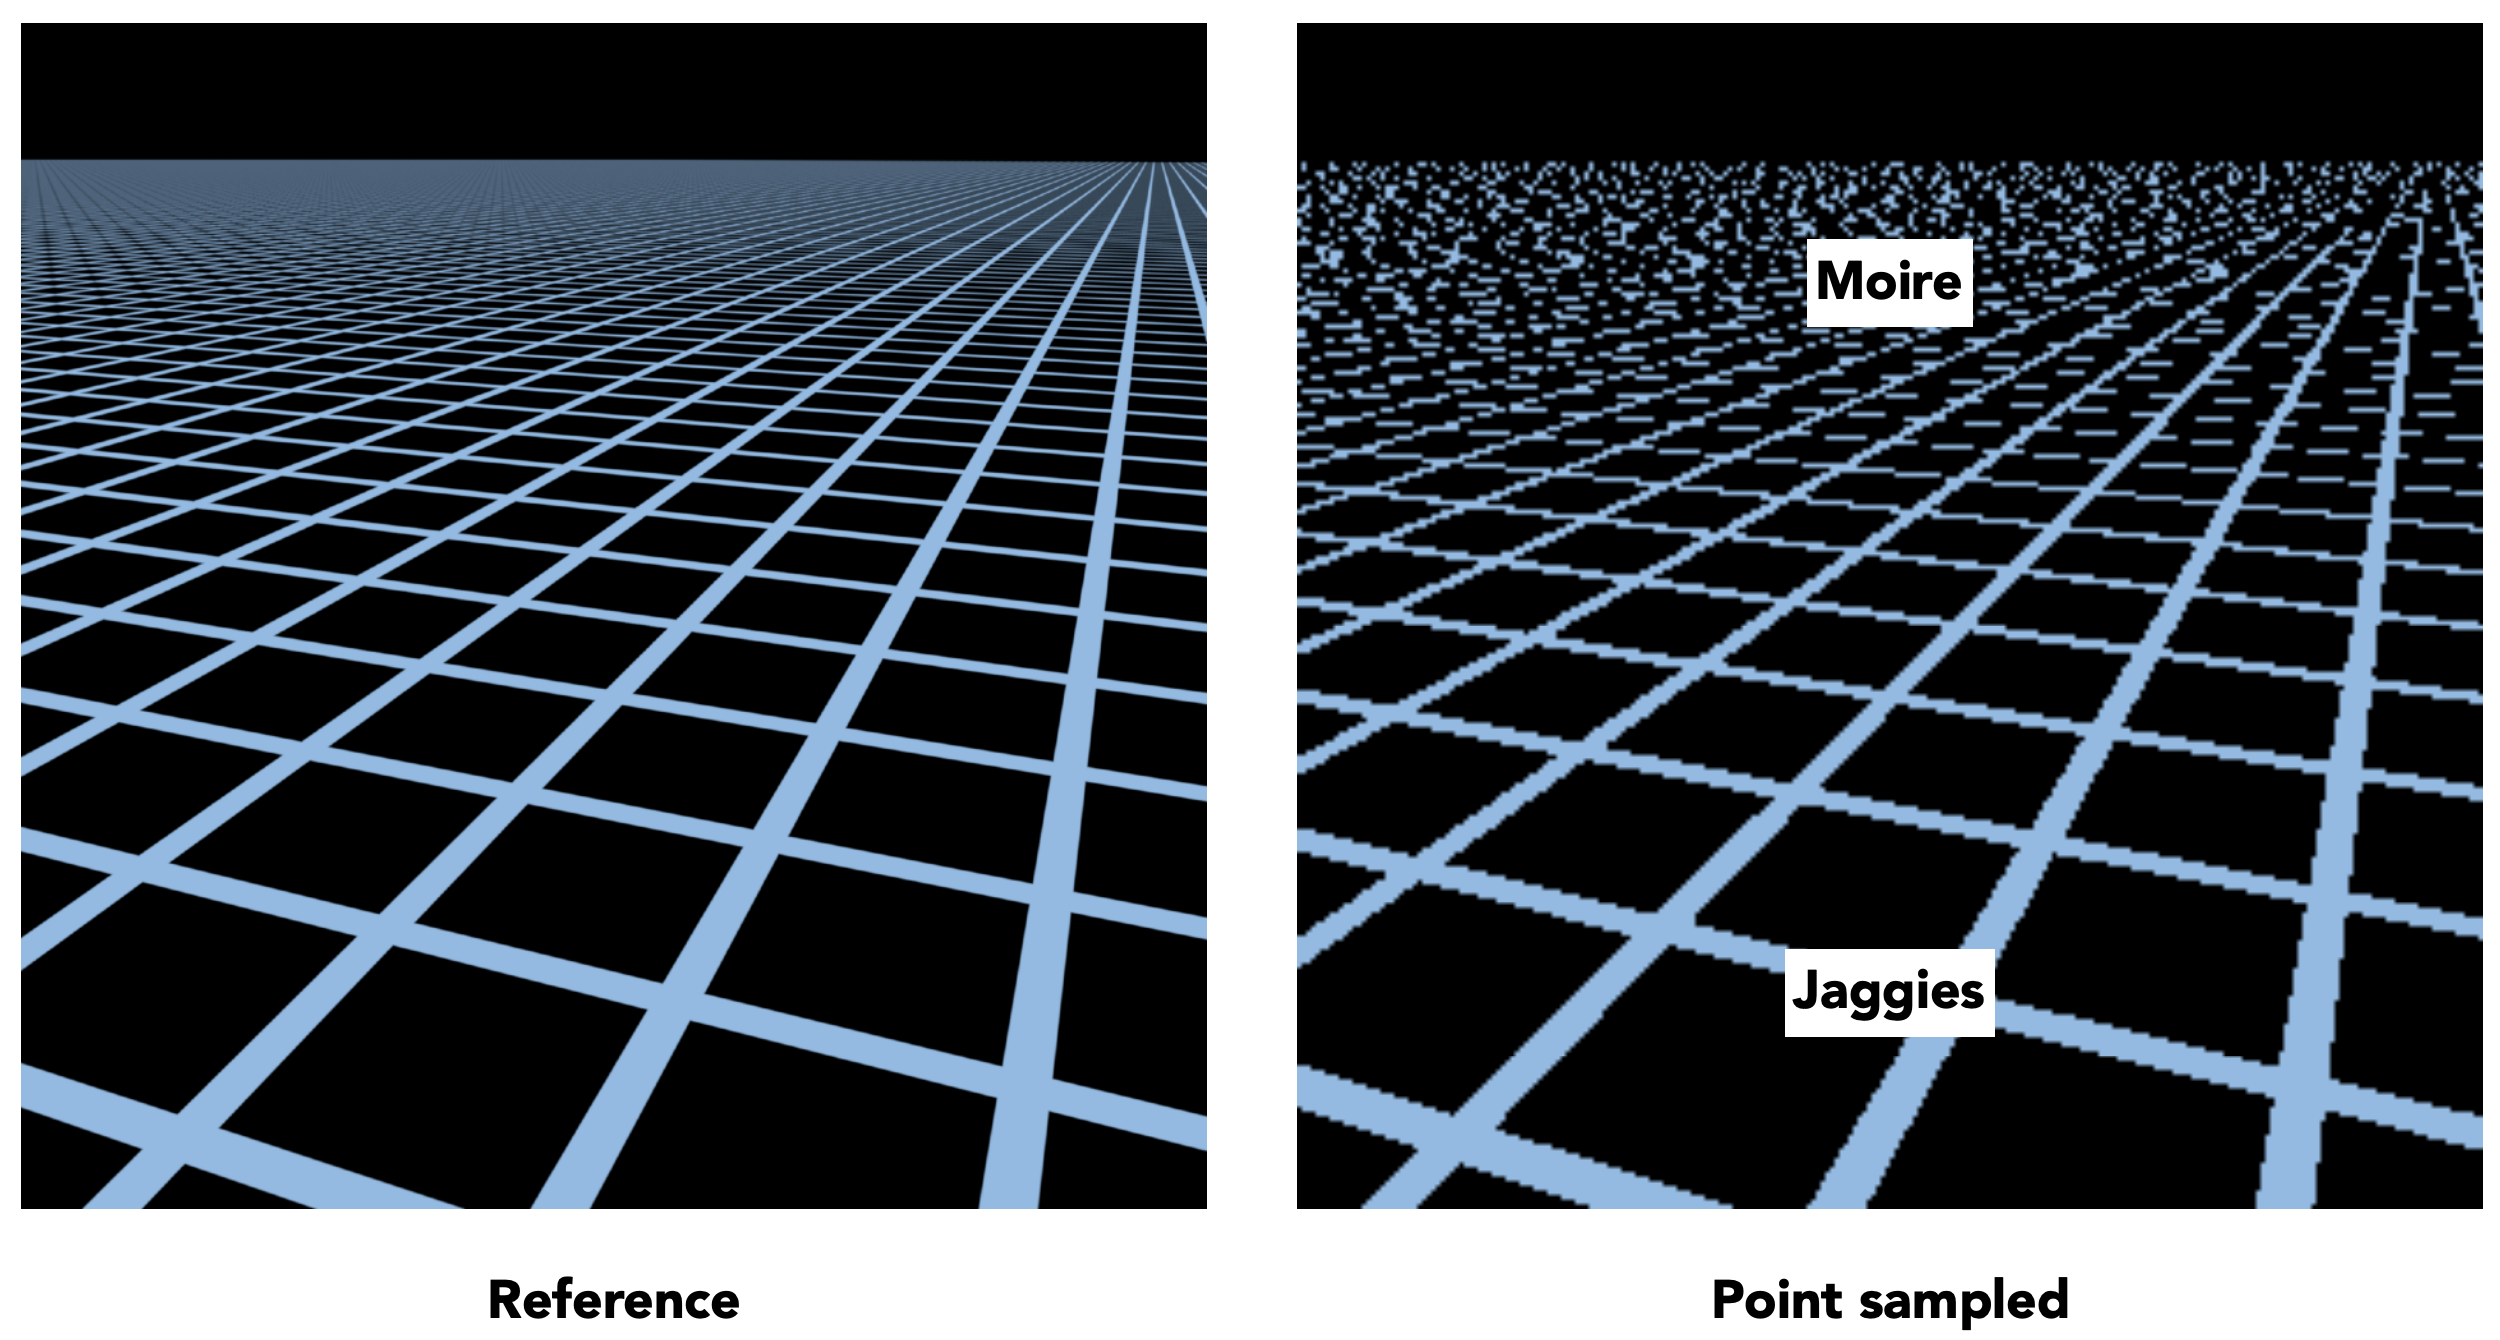
\includegraphics[scale=.15]{dawenli.png}
	\caption{纹理过大结果示意图}
	\label{fig:dawenli}
\end{figure}
我们的解决方法是避免采样。通过像素点直接得到对应纹素区域的平均值。这里我们引入\textbf{Mipmap}来解决这样一个范围查询的问题。Mipmap是一个快速,近似并且只用于正方形区域的范围查询方法。主要思想如下:我们从一张纹理生成一系列的纹理。每一个纹理的大小都是之前纹理大小的一半,最后得到的最小的纹理是一个$1\times 1$的纹理,这就是一个图像金字塔。最终存储这些纹理额外的开销是原本纹理的三分之一。

我们需要计算每一个像素对应纹理的方形大小,并使用对应层的纹理。
\begin{figure}[H]
	\centering
	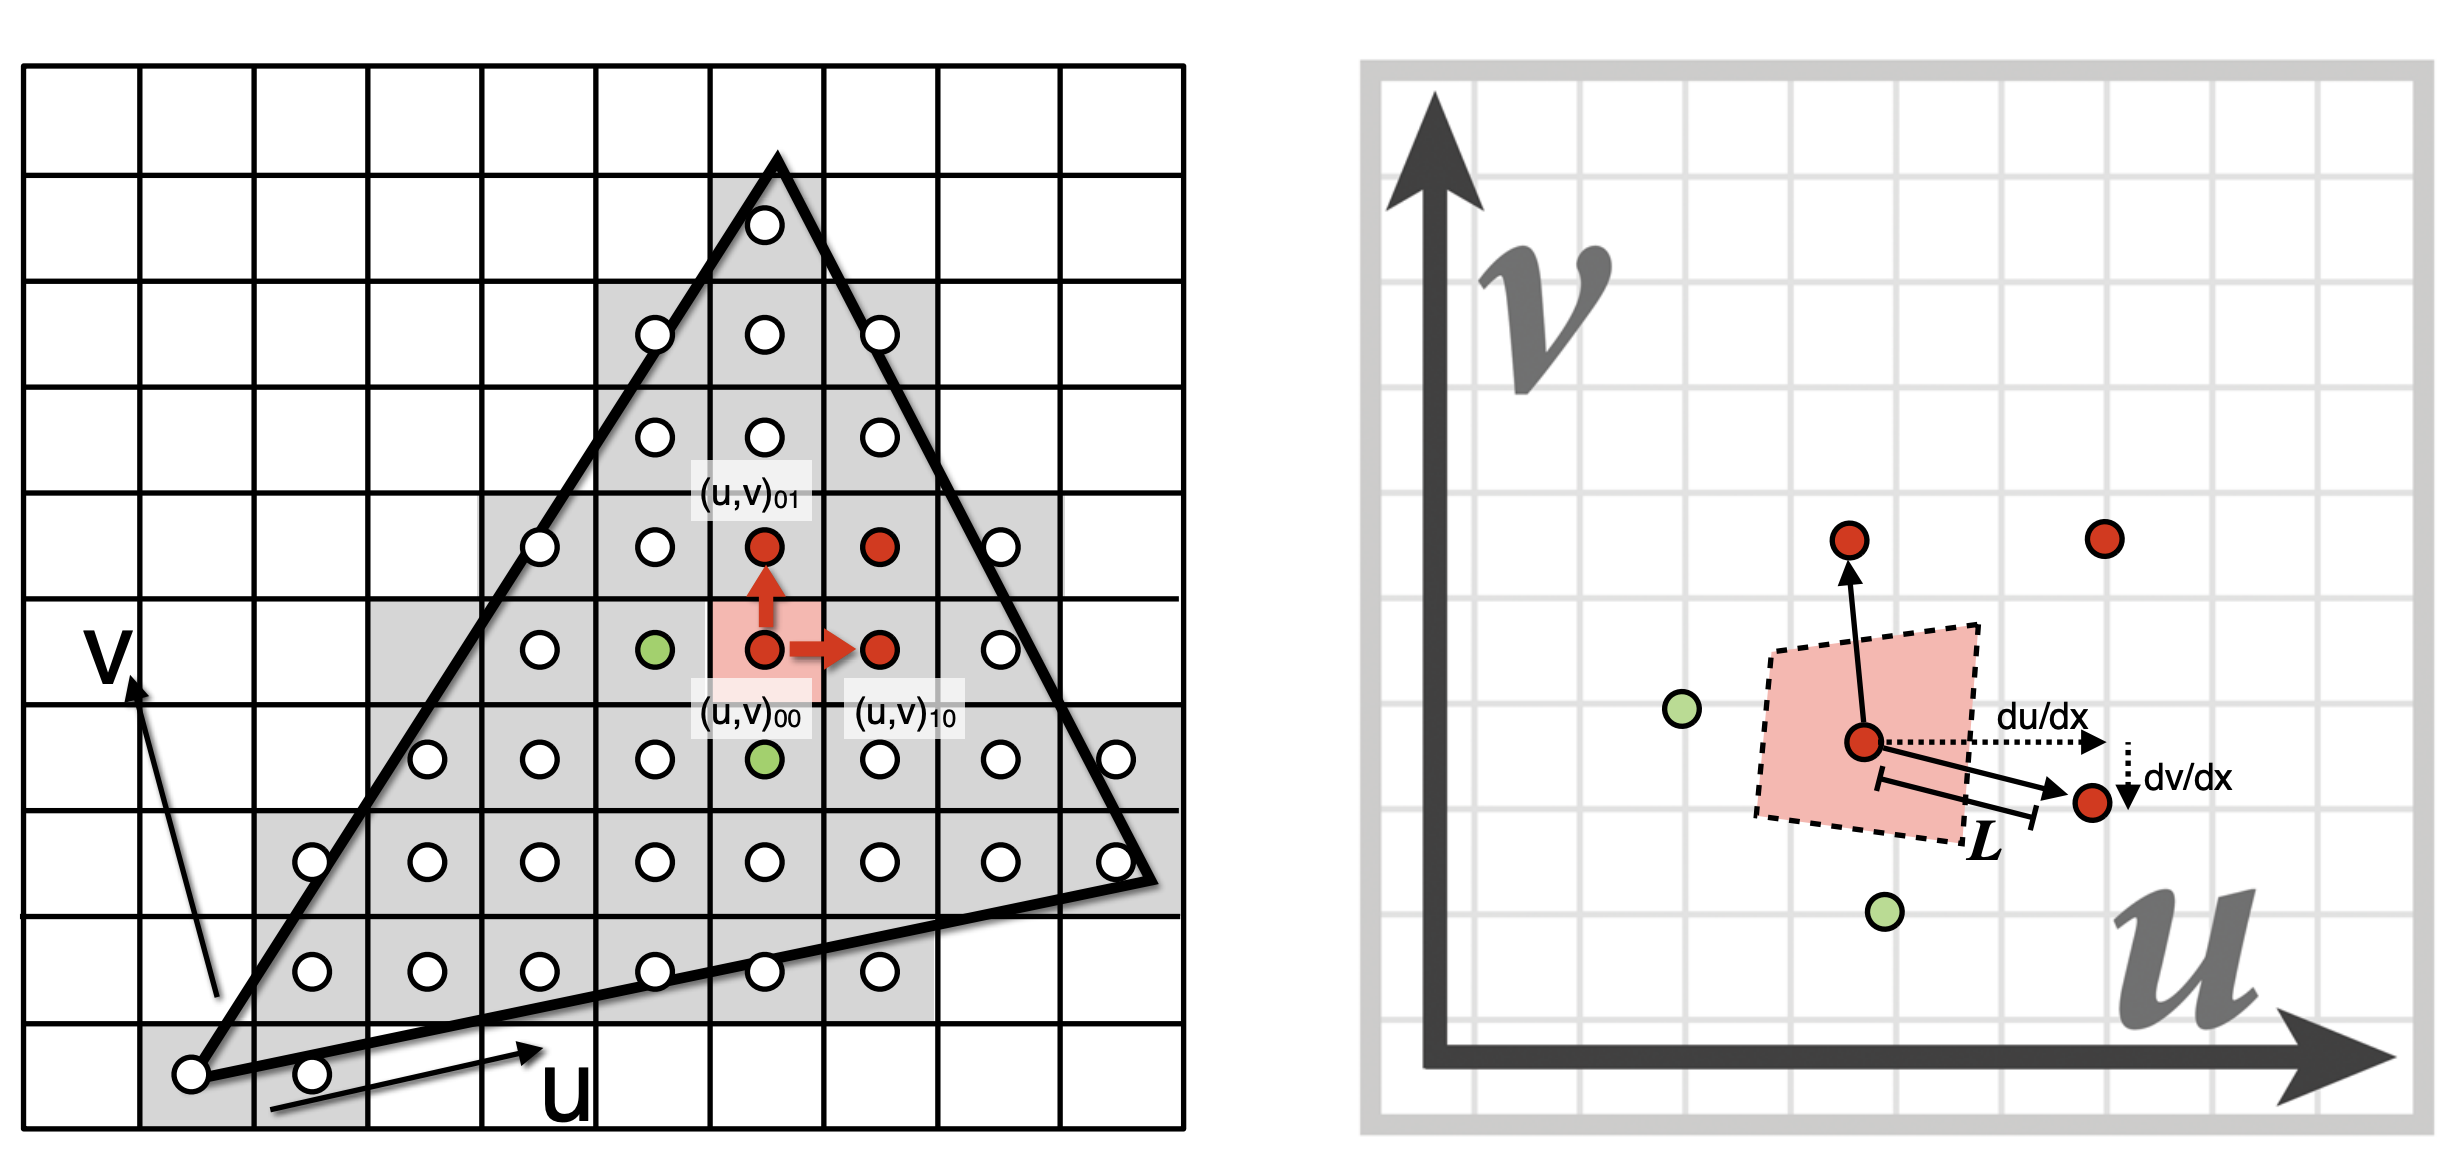
\includegraphics[scale=.3]{mipmap.png}
	\caption{Mipmap对应层数计算}
	\label{fig:mipmap}
\end{figure}
对于一个点$u(0,0)$何其相邻的两个点之间在纹理上的距离,可以用微分形式表示,那么这个像素所对应纹理方形的大小是:
\begin{equation}
	L= \text{max}(\sqrt{(\frac{du}{dx})^2+(\frac{dv}{dx}^2)},\sqrt{(\frac{du}{dy}^2)+(\frac{dv}{dy}^2)})
\end{equation}
那么对应的层数为:$D=\log_2L$。
为了保证我们能够取到的层数是一个连续的层数,我们使用三线性插值法得到对应的结果。首先,对于任意一个非整数层数,我们在其上下两层使用双线性插值进行取值。接下来我们在两个层之间使用线性插值就可以得到最后的结果。

Mipmap也存在局限性。由于所有的纹理都必须对应到一个正方形的区域,但是并不是所有的纹理都可以被一个正方形完美的包住(例如细长的长方形,或者是在对角线上的长方形)。最终远处的纹理会变得非常的模糊,丢失了许多细节。
\begin{figure}[H]
	\centering
	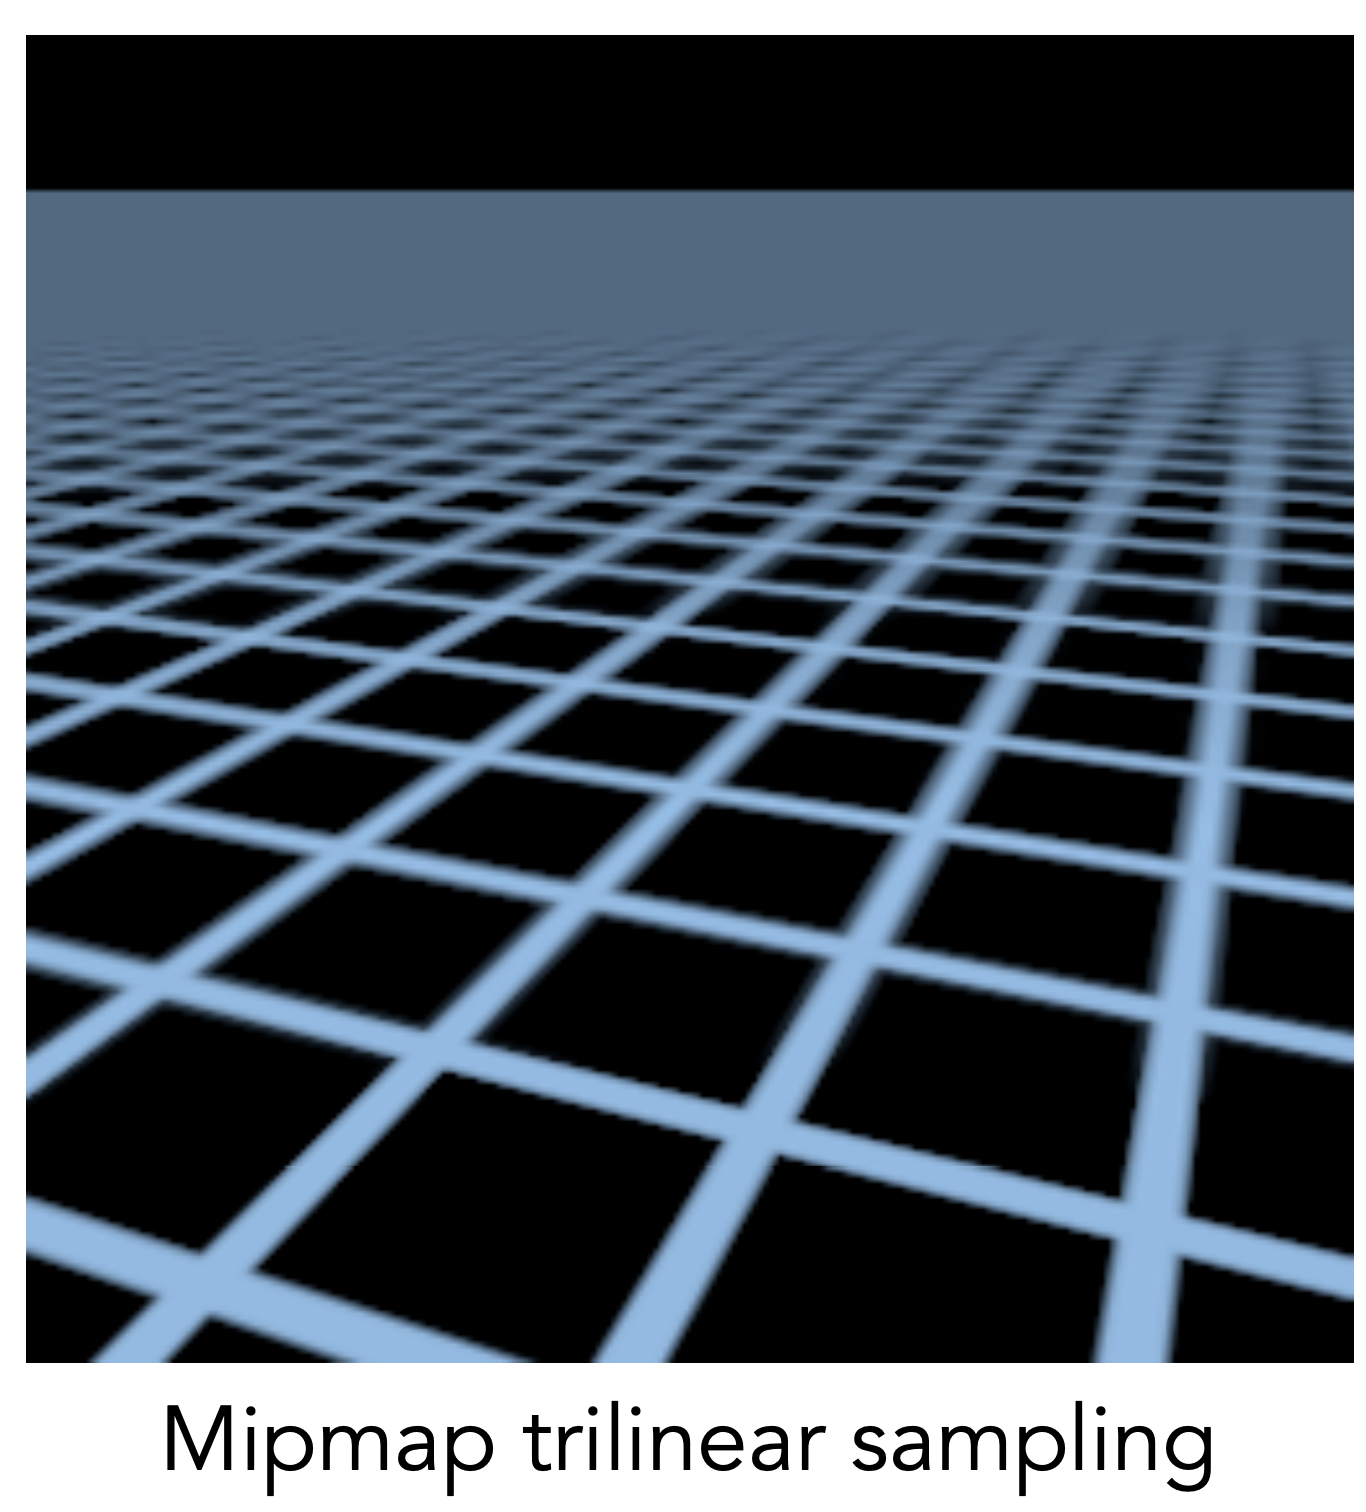
\includegraphics[scale=.2]{mipmapjuxian.png}
	\caption{Mipmap的局限性}
	\label{fig:mipmapjuxian}
\end{figure}
为了解决这个问题,我们使用\textbf{各向异性过滤(Anisotropic Filtering)}解决。各向异性过滤指的是加入只在水平方向或者竖直方向上缩小的纹理,这样可以应对不同长方形纹理块区域。但是对于对角线上的纹理块依然不好解决。并且存储多余的纹理需要多使用原来纹理三倍的开销。
\begin{figure}[H]
	\centering
	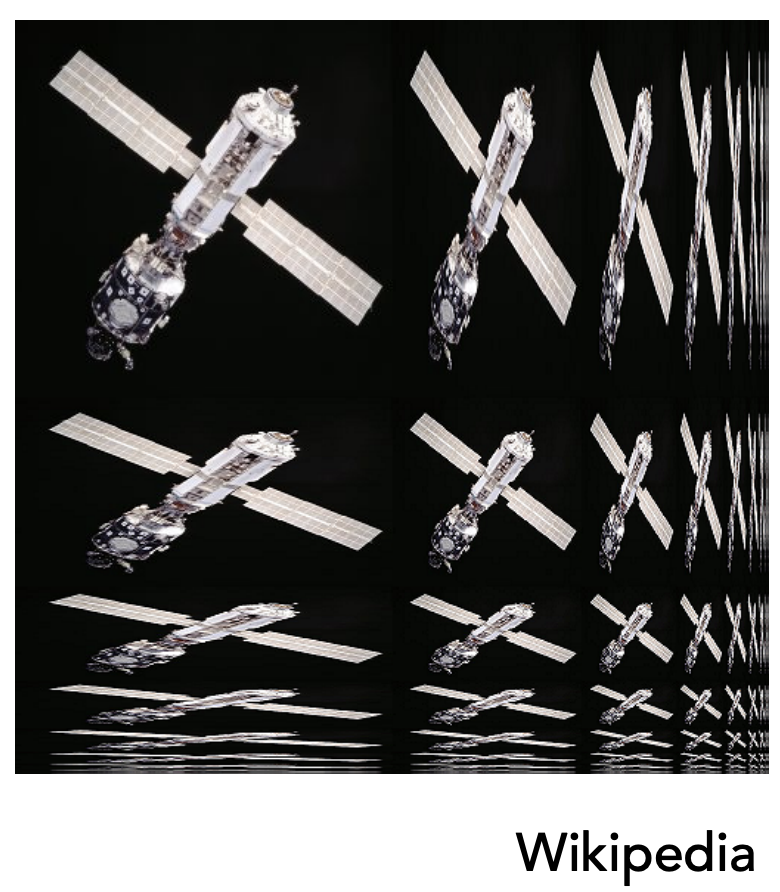
\includegraphics[scale=.3]{gexiangyixing.png}
	\caption{各向异性过滤的纹理图}
	\label{fig:gexiangyixing}
\end{figure}
除此之外我们还可以使用EWA过滤得到更好的结果。可以把纹理拆分成不同的圆形块进行多次查询获得最终的结果。但是开销也会比较大。

\section{纹理的应用}
纹理除了我们所认为是一个“贴图”之外,纹理还有各种各样的应用。纹理是一块内存加上范围查询(滤波)的结果。除了上面简单的纹理应用之外,我们还可以使用纹理做以下事情。

\subsection{环境贴图}
\textbf{环境贴图(Environment Map)}指的是环境中四面八方的情况。可以使用纹理来描述环境光的样子。我们假设环境光来自于无穷远处,没有深度意义。环境光纹理可以看作一个光滑镜面的球表面在环境中所记录的信息。我们需要将球表面展开成一个平面,可以使用两种展开方式:
\begin{figure}[H]
	\centering
	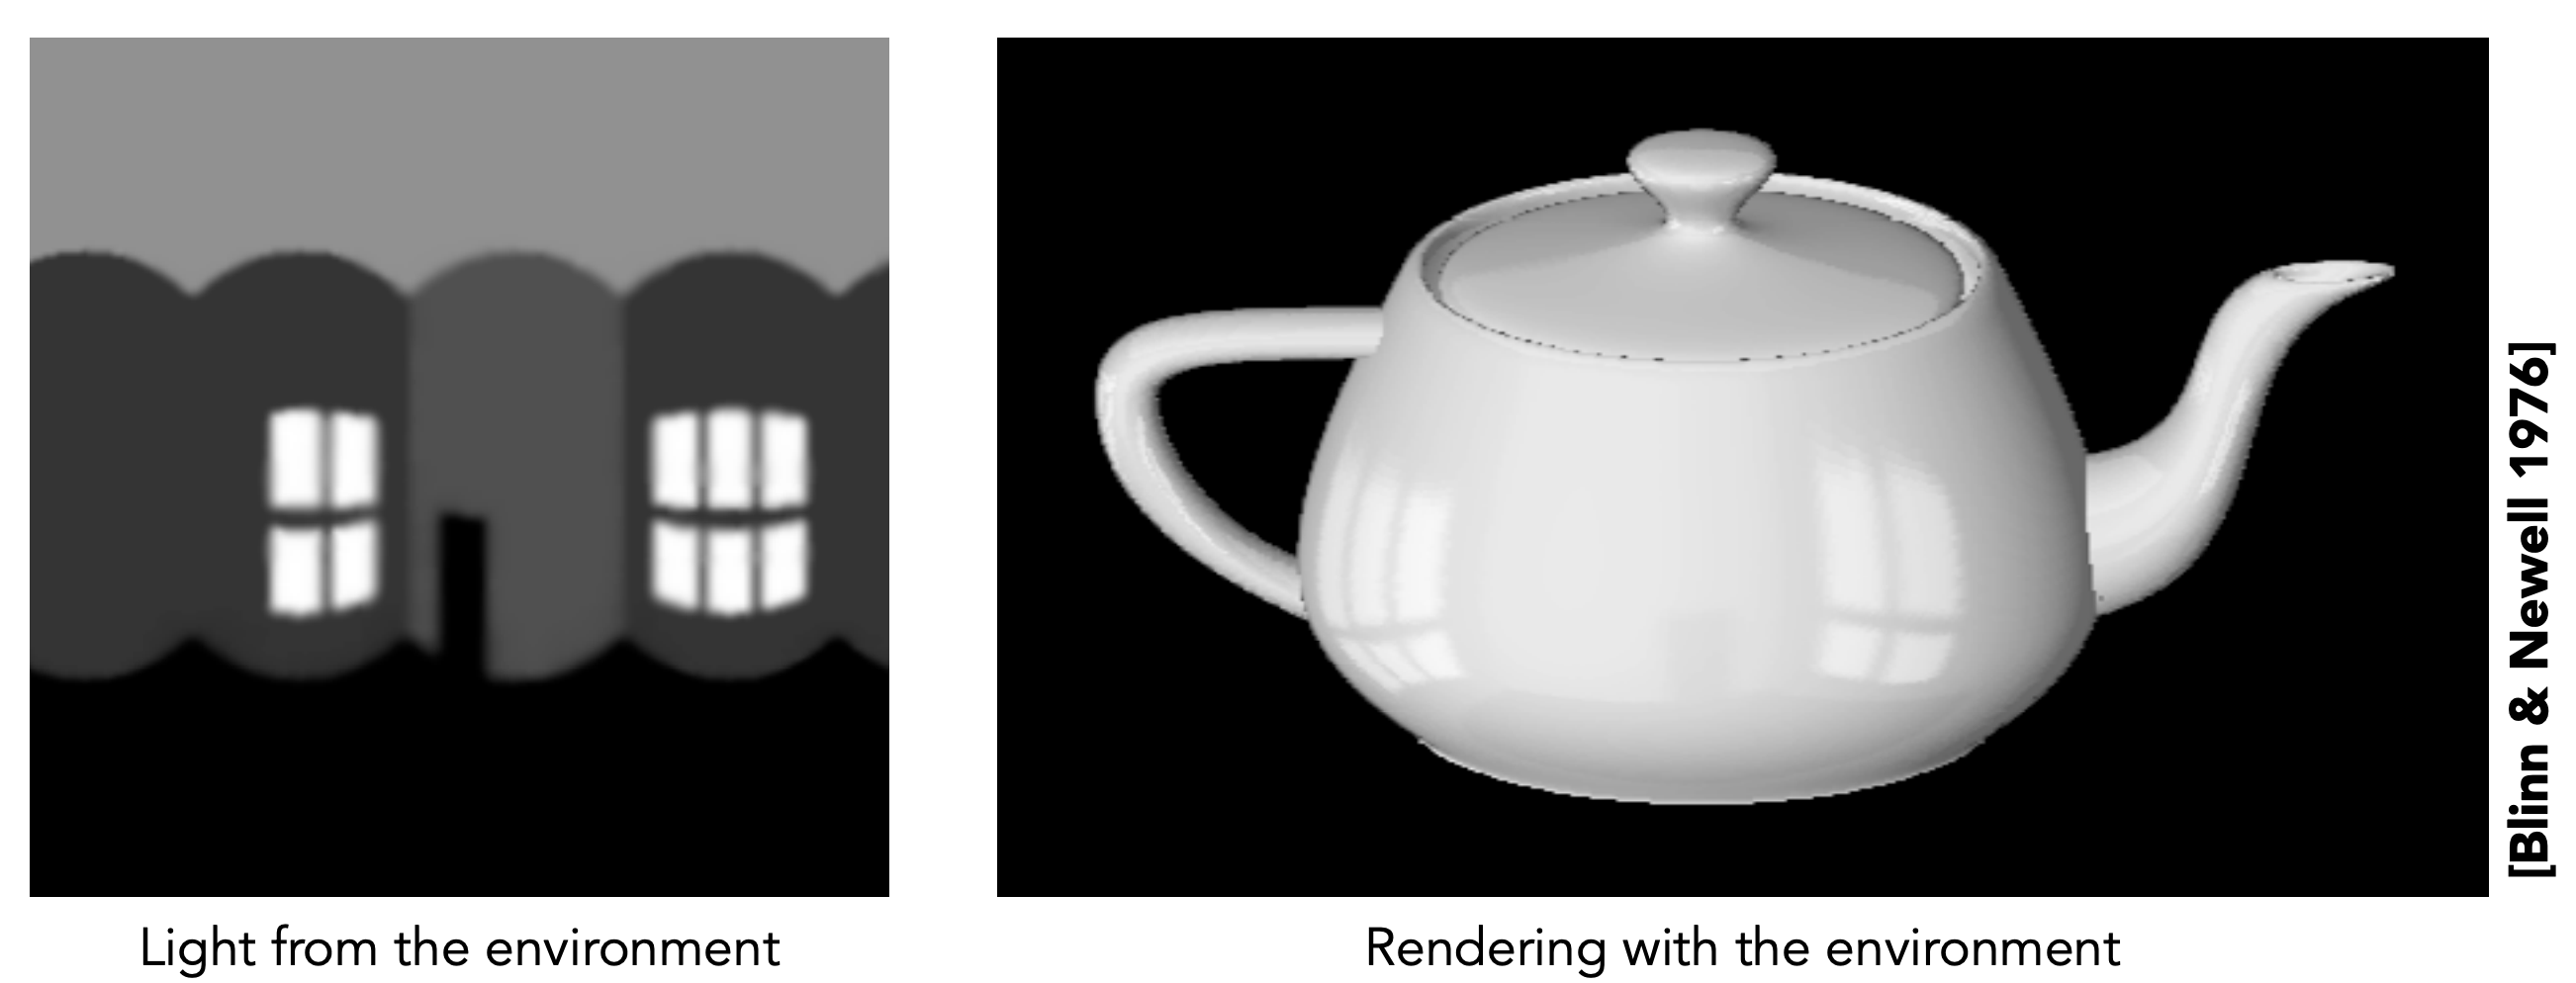
\includegraphics[scale=.2]{huanjingtietu.png}
	\caption{环境贴图示意}
	\label{fig:huanjingtietu}
\end{figure}
\begin{enumerate}
	\item 墨卡托投影法(Mercator Projection):通过将球面映射到一个平面上,我们可以使用墨卡托投影法。墨卡托投影法应用于目前地球仪的投影。它的特点是靠近南北极的地方会发生较大的畸变,这不是一个均匀地描述。
	\begin{figure}[H]
		\centering
		\includegraphics[scale=.2]{mokatuo.png}
		\caption{墨卡托投影法}
		\label{fig:mokatuo}
	\end{figure}
	\item 立方体映射(Cube Map):我们为光滑球定义一个包围盒,将球的平面投影到立方体的六个平面上。这样做就可以得到6张纹理,并且畸变比较小。但是在计算纹素时需要计算球面上的点对应哪一张纹理,判断点和方向的位置关系。
	\begin{figure}[H]
	\centering
	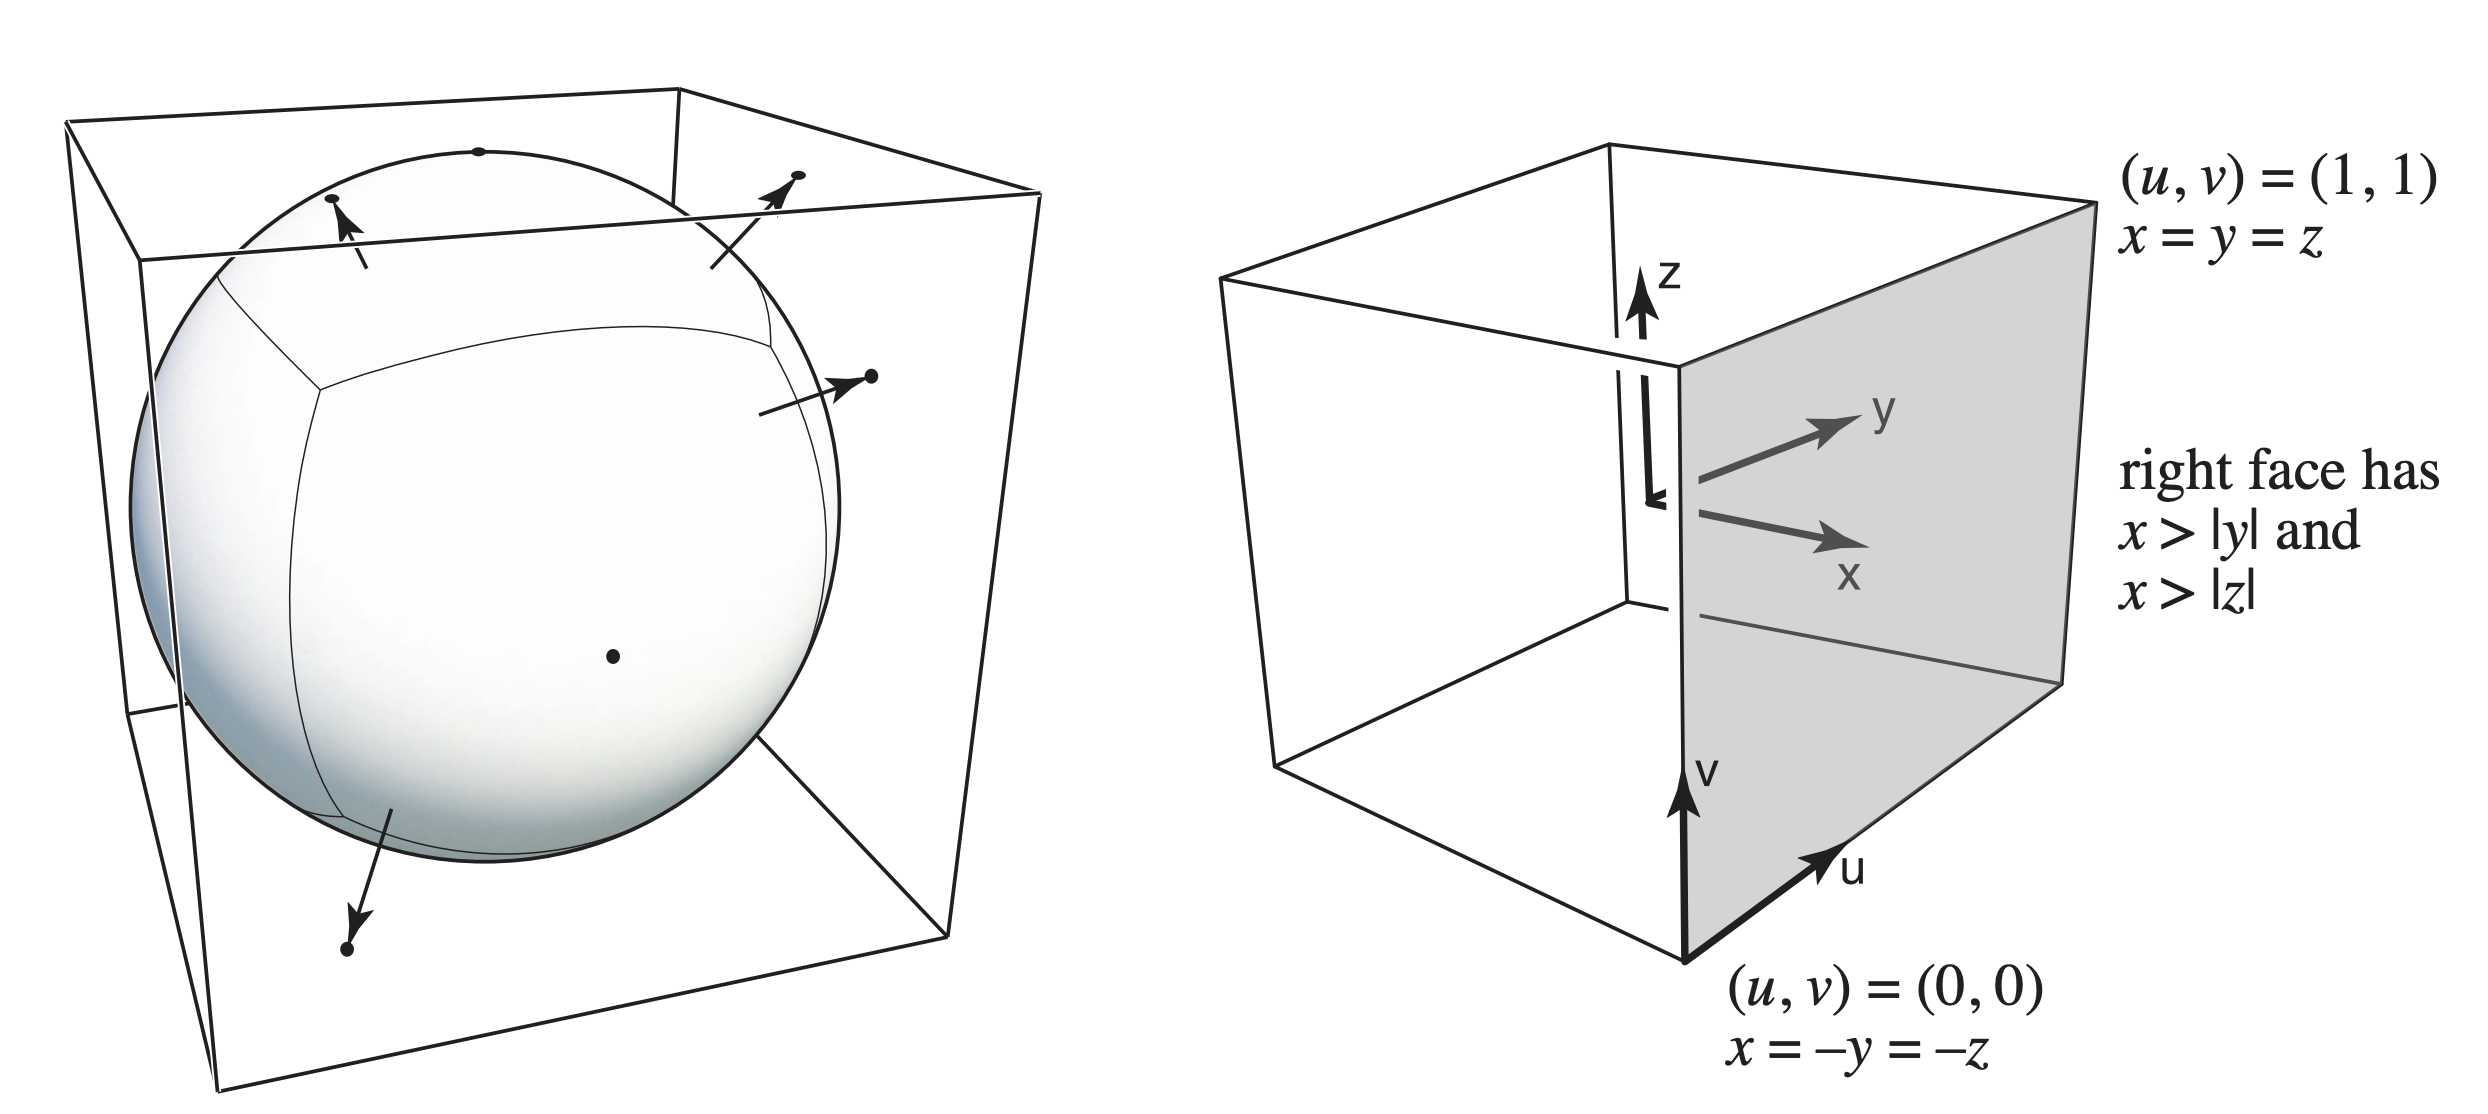
\includegraphics[scale=.15]{cubemap.png}
	\caption{立方体映射}
	\label{fig:cubemap}
	\end{figure}
\end{enumerate}

\subsection{凹凸贴图}
\textbf{凹凸贴图}是指用纹理的方式得到物体表面凹凸不平的感觉,相比于直接通过做出物体凹凸不平的方式,这种方法更加的简单。对于任何一个点,我们只需要改变这个点的法线方向就可以表达出这个点高度的变化。因此这个贴图也被称作\textbf{法线贴图(Bump mapping)}。纹理上的点定义的是点高度的移动,通过纹理上信息我们可以求出新的法线方向。

在二维的情况下,我们假设原物体是一条直线,原始法线方向为$(0,1)$。对于任意一个点$p$,我们定义$p$点的导数是$dp=c\cdot [h(p+1)-h(p)]$。常数$c$定义了凹凸贴图对于法线的影响。那么该点切线的方向是$(1, dp)$。法线的方向和切线的方向成90度角,法线的方向向量是$(-dp, 1)$正则化后的结果。
\begin{figure}[H]
	\centering
	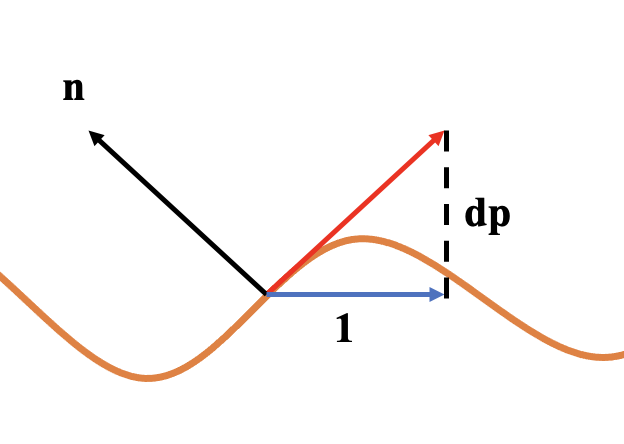
\includegraphics[scale=.5]{aotutietu.png}
	\caption{二维情况下法线贴图中法线的计算}
	\label{fig:aotu}
\end{figure}

推广到三维情况,对于一个原始法线是$(0,0,1)$的平面,我们在u方向和v方向上各做一次求导,结果是$dp/du=c1\cdot [h(u+1)-h(u)],dp/dv=c2\cdot [h(v+1)-h(v)]$。法线的方向是$(-dp/du,-dp/dv,1)$的正则化结果。

对于任意方向的原始法线,我们都可以先按照局部坐标系计算法线后通过变换变换到世界坐标系上。

除了凹凸贴图之外,还有另外一种贴图称作\textbf{位移贴图}。位移贴图会移动所有顶点位置。因此使用顶点贴图的时候模型三角形分的越细越好。凹凸贴图并没有实际改变物体的形状,所以在物体的边上依旧可以看到光滑的曲线。
\begin{figure}[H]
	\centering
	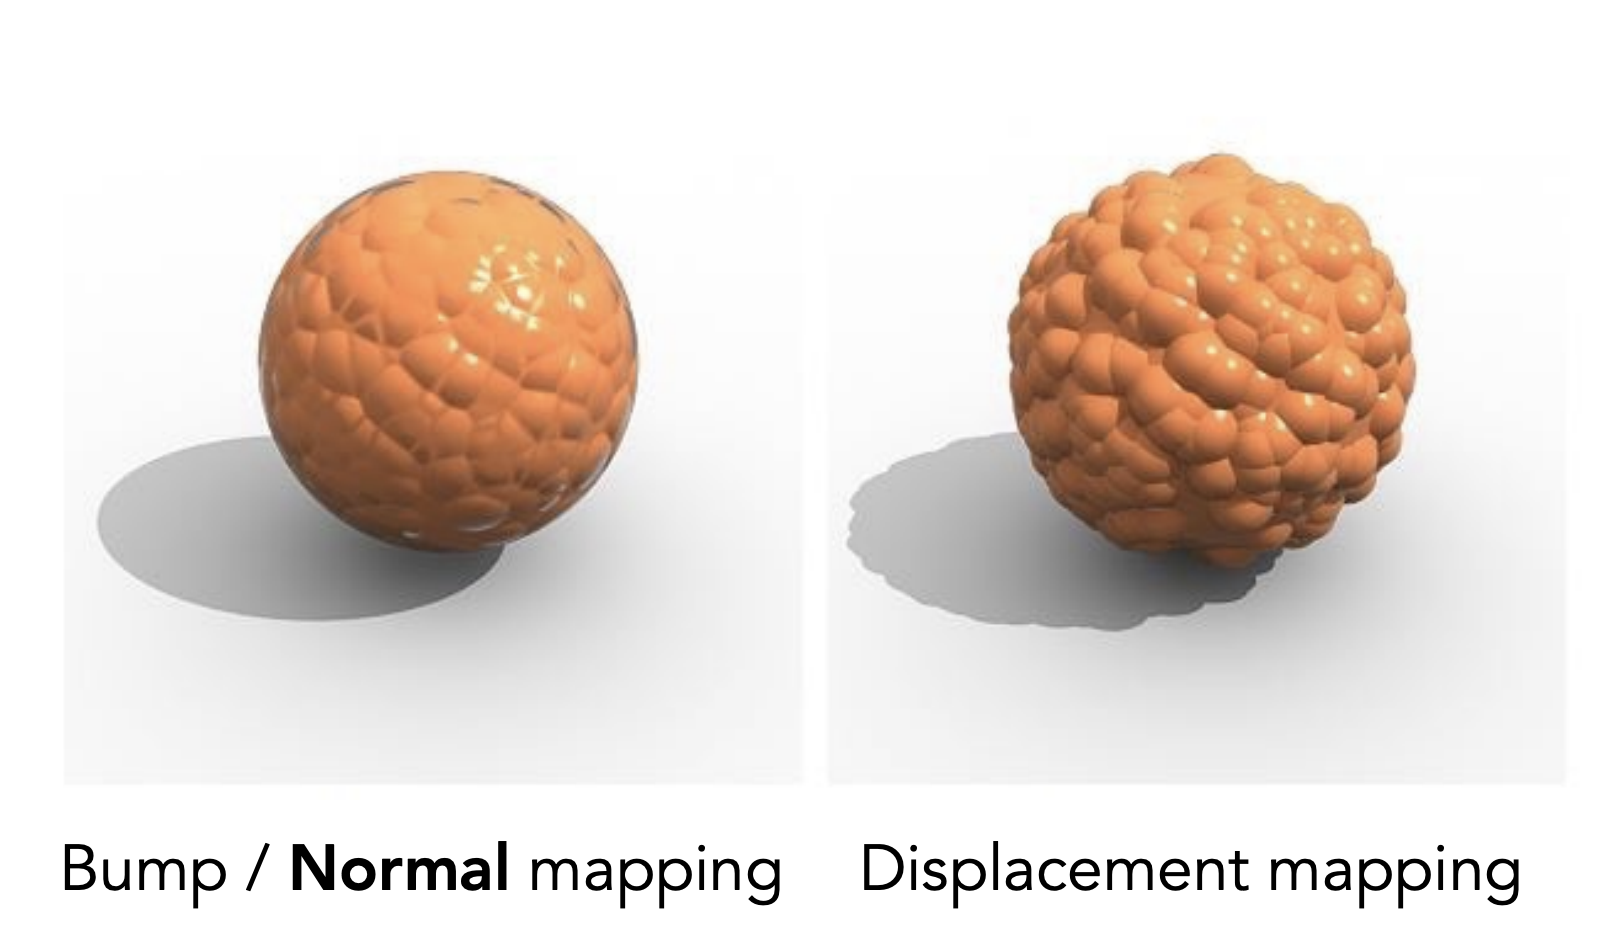
\includegraphics[scale=.3]{weiyitietu.png}
	\caption{凹凸贴图和位移贴图}
	\label{fig:weiyitietu}
\end{figure}

当然,贴图可以推广到三维空间,我们可以使用三维贴图。计算三维空间中任意一个点对应的纹理。

\section{阴影贴图}
贴图还可以直接加入一些阴影,直接计算好贴在纹理上,这样会使得阴影计算变得很快。纹理可以记录一些已经计算好阴影的信息。

\part{几何}
\chapter{几何的描述}

几何主要可以分为两类,一种是\textbf{隐式几何(Implicit Geometry)},一种是\textbf{显式几何(Explicit Geometry)}。

\section{隐式几何}
隐式几何是对点几何进行的描述,并不直接给出点的位置。例如,对于一个单位球面,我们可以使用公式$x^2+y^2+z^2=1$进行表示。我们可以通过函数$f(x,y,z)=0$隐式地定义一个集合。
几何的隐式表示很难看出来所对应的图形,但是可以非常轻松的判断一个点是不是在这个图形面上。隐式几何有以下几种表示方式:
\begin{enumerate}
	\item 使用数学函数表示,是一种不直观的表示方法;
	\item CSG(Constructive Solid Geometry)表示,使用一系列基本几何体通过交、并、差等布尔运算得到最终的结果;
	\item 距离函数(Distance Function)表示,距离函数表现了空间内任意一点到物体的最短距离。两个距离函数的加和可以得到两个物体融合的中间态。非常适合在模拟水滴融合中使用。距离函数中距离为0的平面就是物体平面。距离函数还可以使用水平集(Level Set Method)来离散的表示;
	\item 分型(Fractals)表示,指的是一个图形的一部分和自己整体相比高度相似,可以理解为一种递归的形式。
\end{enumerate}

\section{显式几何}
显式几何通过直接定义几何上的点或者通过把点进行参数映射的方式定义到新的空间(例如我们可以把$u-v$平面上的点映射到三维空间中)。显式几何可以轻松的找到所有的点,但是不好判断空间中任何一个点是否在图形面上。显式几何常见的表示方式有以下几种:
\begin{enumerate}
	\item 点云(Point Cloud)表示,使用一系列空间中三维的坐标来表示物体。点越密集,所形成的模型效果越好。一般会使用点云生成三角形面。
	\item 多面形面(Polygon Mesh)表示,一般使用三角形或者四边形来表示。描述更加复杂但也是最为常用的方式。使用Wavefront Object File(.obj)格式的文件来存储。在obj文件中定义了顶点坐标,法线方向以及纹理坐标还有它们之间的关系。
\end{enumerate}

\chapter{曲线和曲面}
曲线和曲面是常见的几何。在本章将会着重讲解曲线和曲面的表示以及有关的性质。

\section{曲线}
我们使用一系列的点去定义一条曲线。这些控制点描述了曲线的一些性质。最常见的曲线叫做\textbf{贝塞尔曲线(B\'ezier Curve)}。
\subsection{贝塞尔曲线的画法}
\textbf{在三个点的情况下}

在二维情况下,使用三个控制点画出的贝塞尔曲线称为二次贝塞尔曲线(quadratic B\'ezier)。这是由Pierre B\'ezier和Paul de Casteljau提出的算法,称为de Casteljau算法。

\begin{figure}[H]
	\centering
	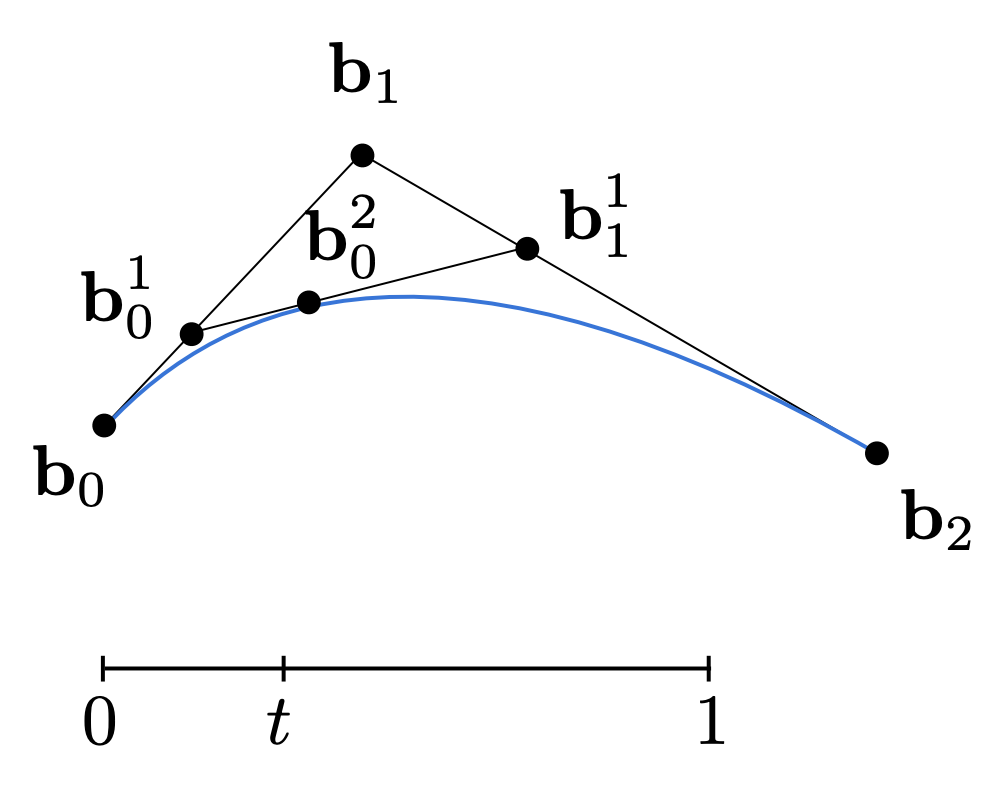
\includegraphics[scale=.3]{beisaier.png}
	\caption{二次贝塞尔曲线的画法}
	\label{fig:beisaier}
\end{figure}
对于$b_0,b_1,b_2$定义的贝塞尔曲线,我们将求贝塞尔曲线的过程转换成求在$t\in [0,1]$时刻,对应贝塞尔曲线上的点。

在某一时刻$t$对应的点可以按照以下方法求出:
\begin{enumerate}
	\item 求出线段$b_0b_1$和线段$b_1b_2$上对应$t$时刻的点$b_0^1,b_1^1$。这个点可以讲线段分割为长度$t$和$1-t$;
	\item 将$b_0^1,b_1^1$连接起来后,重复步骤1即可。点$b_0^2$就是我们得到的最终点。
\end{enumerate}
这是一个递归的计算过程。任何一个点都是时间$t$的一个映射,因此这是显式的几何表示。

\textbf{在多个点的情况下}

在多个点的情况下,我们只需要仿照三个点的情况,每一次都在对应线段上找到对应时刻$t$所对应的点,并将相邻的点连成线段后重复上面的过程,直到得到最后一个点。

\begin{figure}[H]
\centering
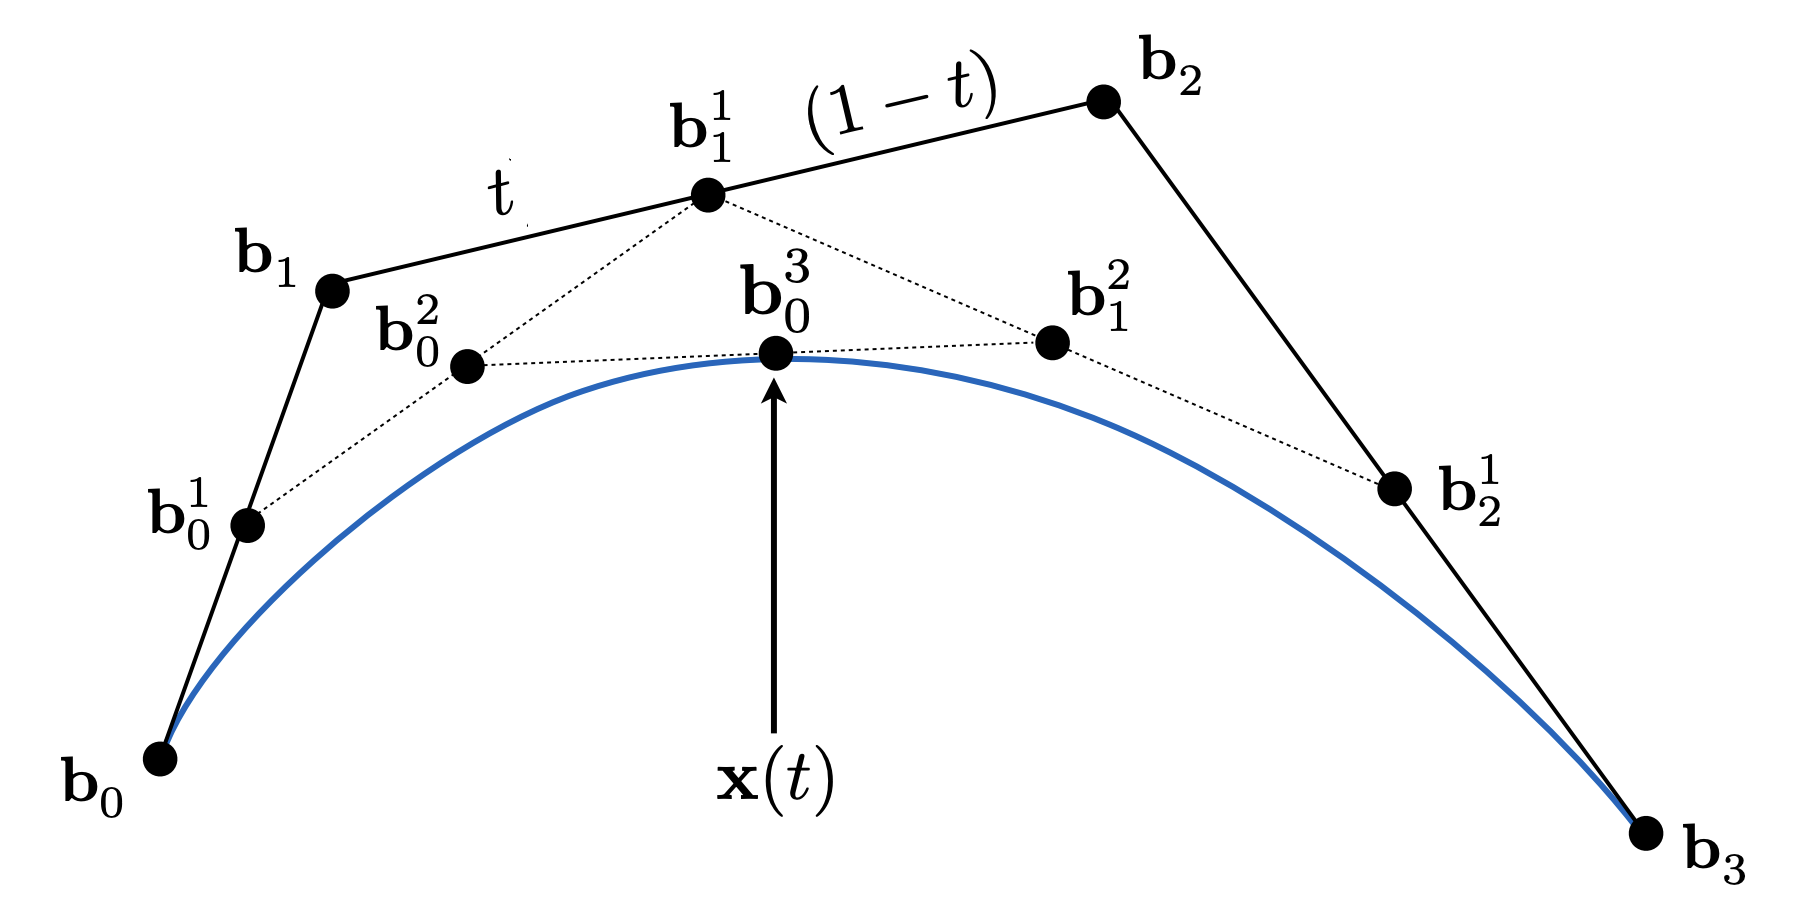
\includegraphics[scale=.15]{beisaier4.png}
\caption{四个控制点确定贝塞尔曲线的画法}
\label{fig:beisaier4}
\end{figure}

\subsection{贝塞尔曲线的数学表示}

通过上一节我们可以看出贝塞尔曲线的画法是类似于递归的方式画出的。我们也知道贝塞尔曲线上的点只和参数$t$有关。因此我们可以得到曲线的数学表示。
\begin{equation}
	b^n=b_0^n=\sum_{j=0}^nb_jB_j^n(t)
\end{equation}
其中$B_j^n(t)$是Bernstein多项式,它是$(t+(1-t))^n$二项分布的第$n$项展开:
\begin{equation}
	B_j^n(t)=\binom{n}{i}t^i(1-t)^{n-i}
\end{equation}

在三维情况下,公式不变。所有的点变成三维空间上的点进行计算即可。

\subsection{贝塞尔曲线的性质}
贝塞尔曲线满足以下性质:
\begin{enumerate}
	\item 贝塞尔曲线必须过起点和终点;
	\item 在四个控制点的情况下,贝塞尔曲线在起点的切线是$b'(0)=3(b_1-b_0)$,终点的切线是$b'(1)=3(b_3-b_2)$;
	\item 对贝塞尔曲线做仿射变换生成的曲线等同于对贝塞尔曲线的控制点做仿射变换后再生成的贝塞尔曲线,这个规律不适用于投影变换;
	\item 凸包性质。画出的贝塞尔曲线一定在控制点所形成的凸包内。凸包是能够包围所有点的最小凸多边形。
\end{enumerate}

\subsection{逐段定义贝塞尔曲线}
当我们使用过多的控制点定义一条曲线时,曲线会变得比较平滑,并且不便控制。因此我们一般使用逐段的方式定义贝塞尔曲线。我们每次使用4个控制点。我们会把前两个点和后两个点各看作一个控制杆来控制整个曲线。这和Photoshop中的钢笔工具是一致的。

对于逐段的贝塞尔曲线,我们需要保证其连续性,我们对连续性有以下定义:
\begin{itemize}
	\item 如果两条分段曲线的起点和终点重合,那么称为C0连接;
	\item 在上面的情况下,如果第一条曲线终点的切线和第二条曲线起点的切线一样,那么称为C1连接;
	\item 在上面的情况下,如果这两个点的n阶导数相同,那么称为Cn连接。
\end{itemize}
一边情况下C1连接就显得足够光滑。在某些特殊情况下我们需要更高阶的连续。

\subsection{样条曲线}
\textbf{样条曲线(Split Curve)}可以形象地理解为在定义了多个控制点后,在这些控制点上固定一个有弹性的木条形成的曲线。在任何一点上不论几阶导数都是连续的。最常见的样条曲线称为B-样条(Basis)。

\section{曲面}
我们可以通过曲线的定义扩展出\textbf{曲面(Surface)}的定义。

\subsection{贝塞尔曲面}
贝塞尔曲面的计算类似于双线性插值的过程。我们使用$4\times 4$个点形成贝塞尔曲面。首先,我们在每一行生成4条贝塞尔曲线,接下来在4条贝塞尔曲线上找到相同时刻对应的4个点生成一条新的贝塞尔曲线。这些贝塞尔曲线的集合形成了贝塞尔曲面。对于贝塞尔曲面,我们需要两个变量$u,v$对其进行数学表示。

\chapter{网格操作}
我们会对模型的网格进行一些操作来达到我们使用的目的。基本的操作包括网格细分(Mesh Subdivision),网格简化(Mesh Simplify)以及网格正则化(Mesh Regularization)。本章将会对前两个操作进行讲解。网格正则化指的是将三角形的平面变成接近于正三角形的一种操作。

\section{网格细分}
\textbf{网格细分(Mesh Subdivision)}会增加更多的三角形面数量,可以看到更多的细节。细分分为两步,第一步是增加三角形的数量,第二步是计算三角形的位置。

\subsection{Loop细分}
Loop细分适用于只有三角形面的模型。首先,每一个三角形面上我们依次连接三条边中点划分为四个新的三角形面。每条边上的中点称为\textbf{新顶点(New Vertex)},原来三角形面上的三个顶点称为\textbf{旧顶点(Old Vertex)}。

对于新顶点和旧顶点,我们采用不同的位置计算方法:

对于非边界上的新顶点,一定被两个三角形面共享。我们假设共享边的顶点是$A,B$,非共享边的两个顶点是$C,D$,那么新顶点的位置是:
\begin{equation}
	\frac{3}{8}(A+B)+\frac{1}{8}(C+D)
\end{equation}

对于旧顶点,假设顶点的度为$n$,原顶点为$O$,周围顶点位置之和为$S$,那么新的顶点位置是:
\begin{equation}
	(1-n\cdot u)\ O+u\ S
\end{equation}
这里,$u=\frac{3}{8n}$。

顶点的计算是一个加权平均的过程,会使整个模型更加的平滑。

\subsection{Catmull-Clerk细分}
Catmull-Clerk细分适用于某些面是非三角形的时候进行细分。我们做出以下定义,如果一个面是四边形,那么称为四边形面,反之为非四边形面。任何一个度不是$4$的点都称为奇异点,反之为非奇异点。

每一次细分我们都在每一条边的中点产生新的顶点,并在每一个面上引入一个中点,将面的中点和边上的中点相连,这就是一次细分操作。这样的细分操作满足一下规律:
\begin{enumerate}
	\item 在第一次细分后,所有原本是非四边形内部都会引入奇异点,并且所有的面都变成了四边形面;
	\item 之后的细分,不会再引入新的奇异点,所有的面都是四边形面。
\end{enumerate}

\begin{figure}[H]
	\centering
	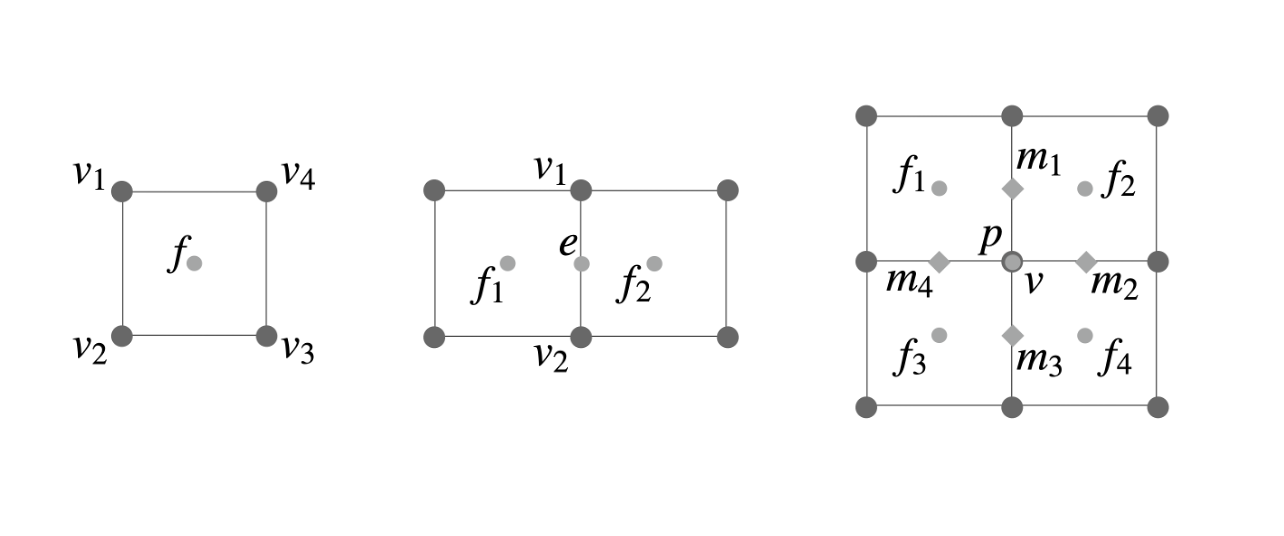
\includegraphics[scale=.4]{xifen.png}
	\caption{Catmull-Clerk细分中,面心,边上的中心以及旧顶点位置的计算}
	\label{fig:xifen}
\end{figure}
这样,对于出现各种形状的面,我们都可以进行细分。这些点新的位置的计算方式如下:
对于面心的点$f$,计算方式为:
\begin{equation}
	f=\frac{v_1+v_2+v_3+v_4}{4}
\end{equation}

对于边上新生成的中点$e$,计算公式为:
\begin{equation}
	e=\frac{v_1+v_2+f_1+f_2}{4}
\end{equation}

对于旧顶点$v$,新的位置的计算公式为:
\begin{equation}
	v=\frac{f_1+f_2+f_3+f_4+2(m_1+m_2+m_3+m_4)+4p}{16}
\end{equation}

\section{网格简化}
\textbf{网格简化(Mesh Simplify)}通过减少模型的面数简化模型。对于一个模型,我们可以通过构造不同的层级,在不同的情况下选择不同的模型。

我们使用\textbf{坍缩(Collapsing)}的方式进行网格简化。我们将边坍缩变成一个点。我们希望这个点和旧顶点连接后与之前的形状差不多,因此我们引入二次误差度量(Quadric Error Metrics)来度量任意一点与旧顶点连接后与原来的相似程度,并选择最小值作为结果。

在模型中,当我们进行坍缩的时候,我们会对所有可以坍缩的点进行排序,每一次探索误差最小的点后,更新这个点周围的点新的误差值。这里采用堆或者优先队列的方式进行实现。

网格简化是一种贪心算法,我们使用局部的最优解并认为是全局最优的结果。

\part{光线追踪}

\chapter{阴影}

在着色这一部分,我们介绍了如何对各个物体计算对应像素的颜色。然而,我们的计算对于每个模型来说都是独立的,并没有考虑光的遮挡关系。因此我们在这里说明在光栅化的情况下,如何计算阴影。

\section{Shadow Mapping}
\textbf{Shadow Mapping}是一种图像空间的算法。在计算阴影的时候我们不需要知道场景的几何信息。Shadow Mapping的方法只适用于在点光源下计算硬阴影。硬阴影指的是一个点是否在阴影内是确定的,它不是在阴影内就在阴影外;只有点光源才可以产生这种情况。软阴影指的是阴影是有过渡的,一个点可以接收到部分光线;当不忽略光源大小的时候,就会产生这种情况。可以接收到部分光线的区域一般称为半影。

一个点是否在阴影中取决于光源和摄像机是不是都可以看到这个点。如果都可以看到这个点,那么说明这个点不在阴影里。因此我们使用如下方式进行计算:
\begin{enumerate}
	\item 从光源位置看向场景,做出深度图;
	\item 从摄像机位置看向场景,对于每一个看到的点,计算到光源的距离,并且得到光源深度图上对应像素点的距离进行比较。如果距离一样,那么说明这个点不在阴影中,反之,这个点在阴影中。
\end{enumerate}

这样的算法有两个问题:
\begin{enumerate}
	\item 距离是一个浮点数,不容易进行比较。需要引入一定的宽容度。这是数值精度的问题,不能从本质解决问题;
	\item 阴影的质量和光源深度图的分辨率有关。如果光源深度图太小,但是摄像机分辨率大就容易出现走样问题;
	\item 这个方法只适合硬阴影,不适合软阴影。
\end{enumerate}

因此,我们需要引入光线追踪的方法来解决光栅化Shadow Mapping中可能出现的问题。

\chapter{光线追踪}

\section{基础知识}

我们引入光线追踪,主要是为了解决光栅化中没有解决的一些问题:
\begin{enumerate}
	\item 全局的光照效果不好表示;
	\item 软阴影效果的产生;
	\item 光泽反射(Glossy reflection,一种类似于镜面反射的情况,但是没有镜面光滑的表面产生的情况)会让光线在场景中多次反射;
	\item 间接光照,在漫反射场景中,有些光线在到达眼睛前反射不止一次。
\end{enumerate}

光栅化是一种比较快速,近似的一种渲染方式,用于实时渲染;光线追踪是比较准确但是比较慢的渲染方式,用于离线渲染。

\subsection{基本光线追踪方法}

\subsubsection{光线的定义}

我们假设光线有以下三个性质:
\begin{enumerate}
	\item 光沿直线传播;
	\item 光线和光线不会发生碰撞的交叉;
	\item 光线从光源射入人眼中。
\end{enumerate}
因此我们可以利用光的可逆性(Reciprocity)进行光线追踪。光线追踪是指我们从摄像机沿着每一个像素点的连线射出光线,追踪光线的路径。

\subsubsection{光线追踪的假设}
我们认为眼睛是一个点,光源均为点光源。我们从眼睛沿着像素点画一条光线,如果光线和物体有接触,我们将交点和光源进行连线,如果可以连接到光源,那我们认为这一点被照亮,可以计算着色。

\subsection{Whitted-Style光线追踪}
从眼睛沿着像素连接一条光线,我们认为光线在传播的过程中发生反射和折射现象。假设反射是完美的镜面反射。当我们将所有的反射(折射)点和光源连接起来。如果这一点可以被光源照亮,那么我们认为这一点的着色应当叠加在这个像素上。对于光线我们认为存在能量的消逝,不会一直反射。

\begin{figure}[H]
	\centering
	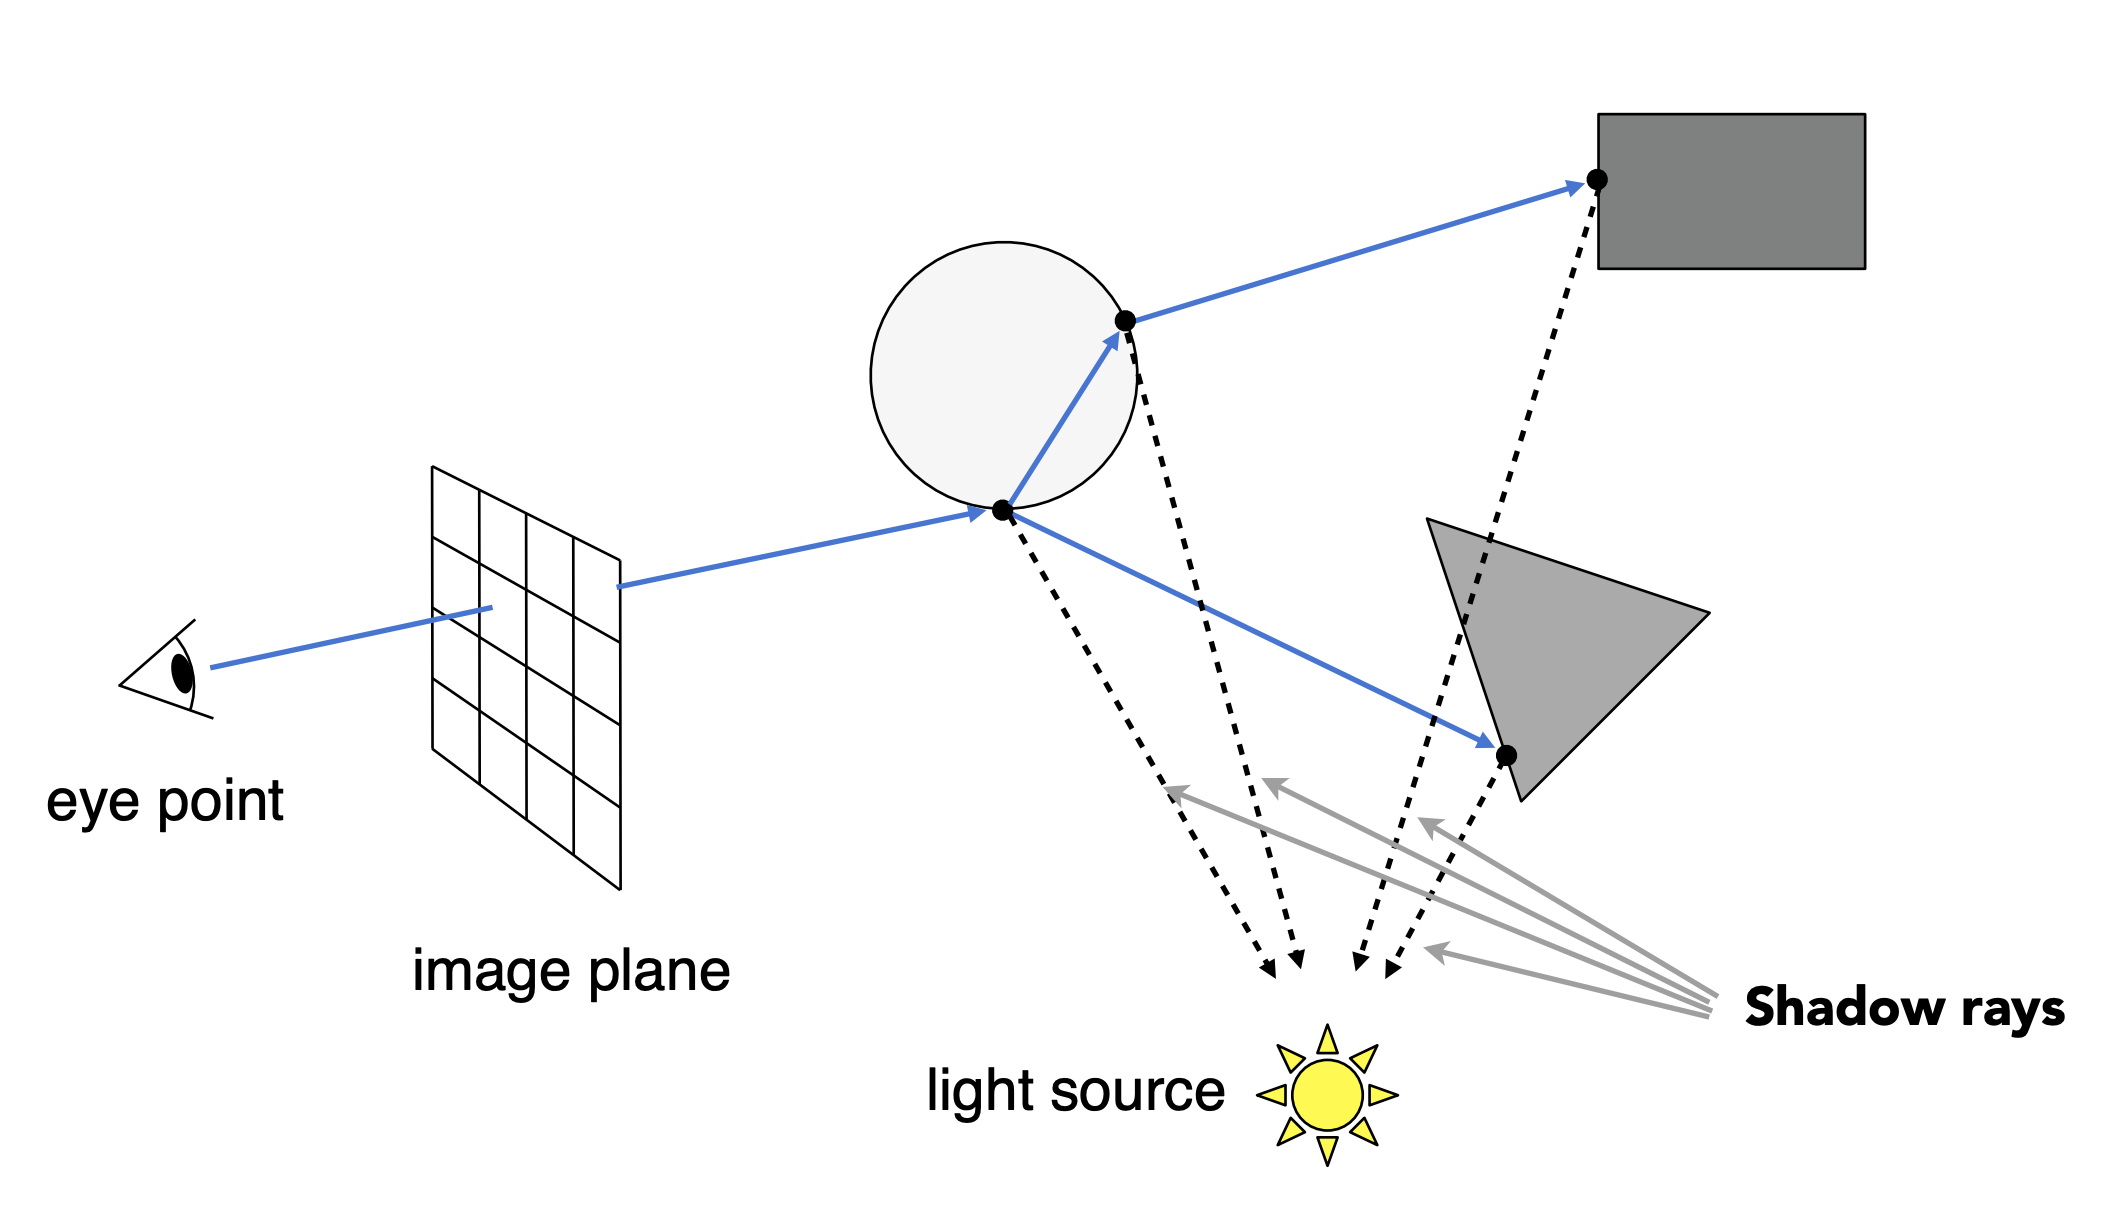
\includegraphics[scale=.25]{guangxianzhuizong.png}
	\caption{Whitted-Style光线追踪示意图}
	\label{fig:gxzz}
\end{figure}
眼睛和像素直接连接起来的光线称为primary ray,发生反射和折射后形成的光线称为secondary ray,反射点和光源的连线称为shadow ray。

\subsection{光线-表面交点}
对于光线追踪而言,最重要的就是求出光线和物体的交点。首先我们对光线进行定义。我们假设光线的起点为$o$,光线的方向是单位向量$d$,那么光线就可以定义为$o+td$。

\subsubsection{光线和球面的交点}

我们首先计算光线和球面的交点作为引入。光线我们可以表示为:
\begin{equation}
	r(t)=o+td, 0\le t \le \infty
\end{equation}

对于球面,我们可以表示为:
\begin{equation}
	(p-c)^2-R^2=0
\end{equation}其中,$c$是球心,$p$是任意一点。如果$p$是光线和球面的交点,那么这个点可以同时满足上面两个函数。因此,我们将光线公式代入到球面公式上就可以得到它们的交点:
\begin{equation}
	(o+td-c)^2-R^2=0
\end{equation}
这是一个二元一次方程组,使用求根公式就可以得到结果。我们讨论求根公式中$\triangle$值。如果$\triangle < 0$,那么光线和球体没有交点;如果$\triangle = 0$,光线和球体相切;如果$\triangle > 0$,那么光线穿过球体,有两个交点。

\subsubsection{光线和隐式函数面的交点}

光线我们可以表示为:
\begin{equation}
	r(t)=o+td, 0\le t \le \infty
\end{equation}

对于任意一个隐式函数面,我们定义为:
\begin{equation}
	f(p)=0
\end{equation}

我们可以直接把光线公式代入隐式函数中求出结果:
\begin{equation}
	f(o+td)=0
\end{equation}

\subsubsection{光线和显式三角形面的交点}
我们可以通过求交点的方式判断一个点是否在封闭曲面的内部还是外部。任何一个点发出一条光线,如果交点个数为奇数,那么这个点一定在封闭曲面内部;如果有偶数个点,那么这个点一定在封闭曲面的外部。

我们求一条光线和显式三角形面的交点可以分为两步:
\begin{enumerate}
	\item 求出光线和三角形面所在平面的交点;
	\item 判断这个点是否在三角形内(之前的课程中已经介绍了判断的方法)。
\end{enumerate}

我们使用法线$N$和平面上的任意一个点$p‘$来定义一个平面:
\begin{equation}
	(p-p')\cdot N = 0
\end{equation}
其中$p'$是平面上任意一点,满足条件的$p$都在这个平面上。我们令$p=o+td$就可以求出光线和这个平面的交点,
\begin{equation}
	(p-p')\cdot N = (o+td-p')\cdot N = 0
\end{equation}
可以求出:
\begin{equation}
	t = \frac{(p'-o)\cdot N}{d\cdot N}, 0\le t \le \infty
\end{equation}

我们可以通过另一种算法直接求出一条光线和一个显式三角形面是否有交点。任何一个显式的三角形内部的一个点都可以写成三个顶点的线性组合。因此我们可以得到:
\begin{equation}
	o+td=(1-b_1-b_2)P_0+b_1P_1+b_2P_2
\end{equation}使用克莱姆法则可以得到:
\begin{equation}
	\begin{bmatrix}
		t\\ 
		b_1\\ 
		b_2
	\end{bmatrix}=\frac{1}{S_1\cdot E_1}\begin{bmatrix}
		S_2\cdot E_2\\ 
		S_1\cdot E\\ 
		S_2\cdot D
	\end{bmatrix}
\end{equation}其中,$E_1=P_1-P_0,E_2=P_2-P_0,S=O-P_0,S_1=D\times E_2, S_2=S\times E_1$.最后我们只需要判断这个解是否合理即可,只要求解出的三个量都是非负的,那么光线和显式三角形面有一个交点。

\section{光线追踪加速}
传统的计算方法所需要的计算消耗量非常大,因此我们需要通过一些方式加速计算。
\subsection{包围体积}
\textbf{包围体积(Bounding Volume)}使用一个简单的立方体包围复杂的模型。如果光线连包围盒都碰不到,那么光线一定不能碰到里面的物体。
我们常用的包围盒是\textbf{轴对其包围盒(Axis-Aligned Bounding Box, AABB)},包围盒的长宽高和坐标轴都是平行的。我们认为,包围体积是三组成对平面的交集。为了计算光线和包围盒的相交情况,我们在二维情况下进行简化计算:
\begin{figure}[H]
	\centering
	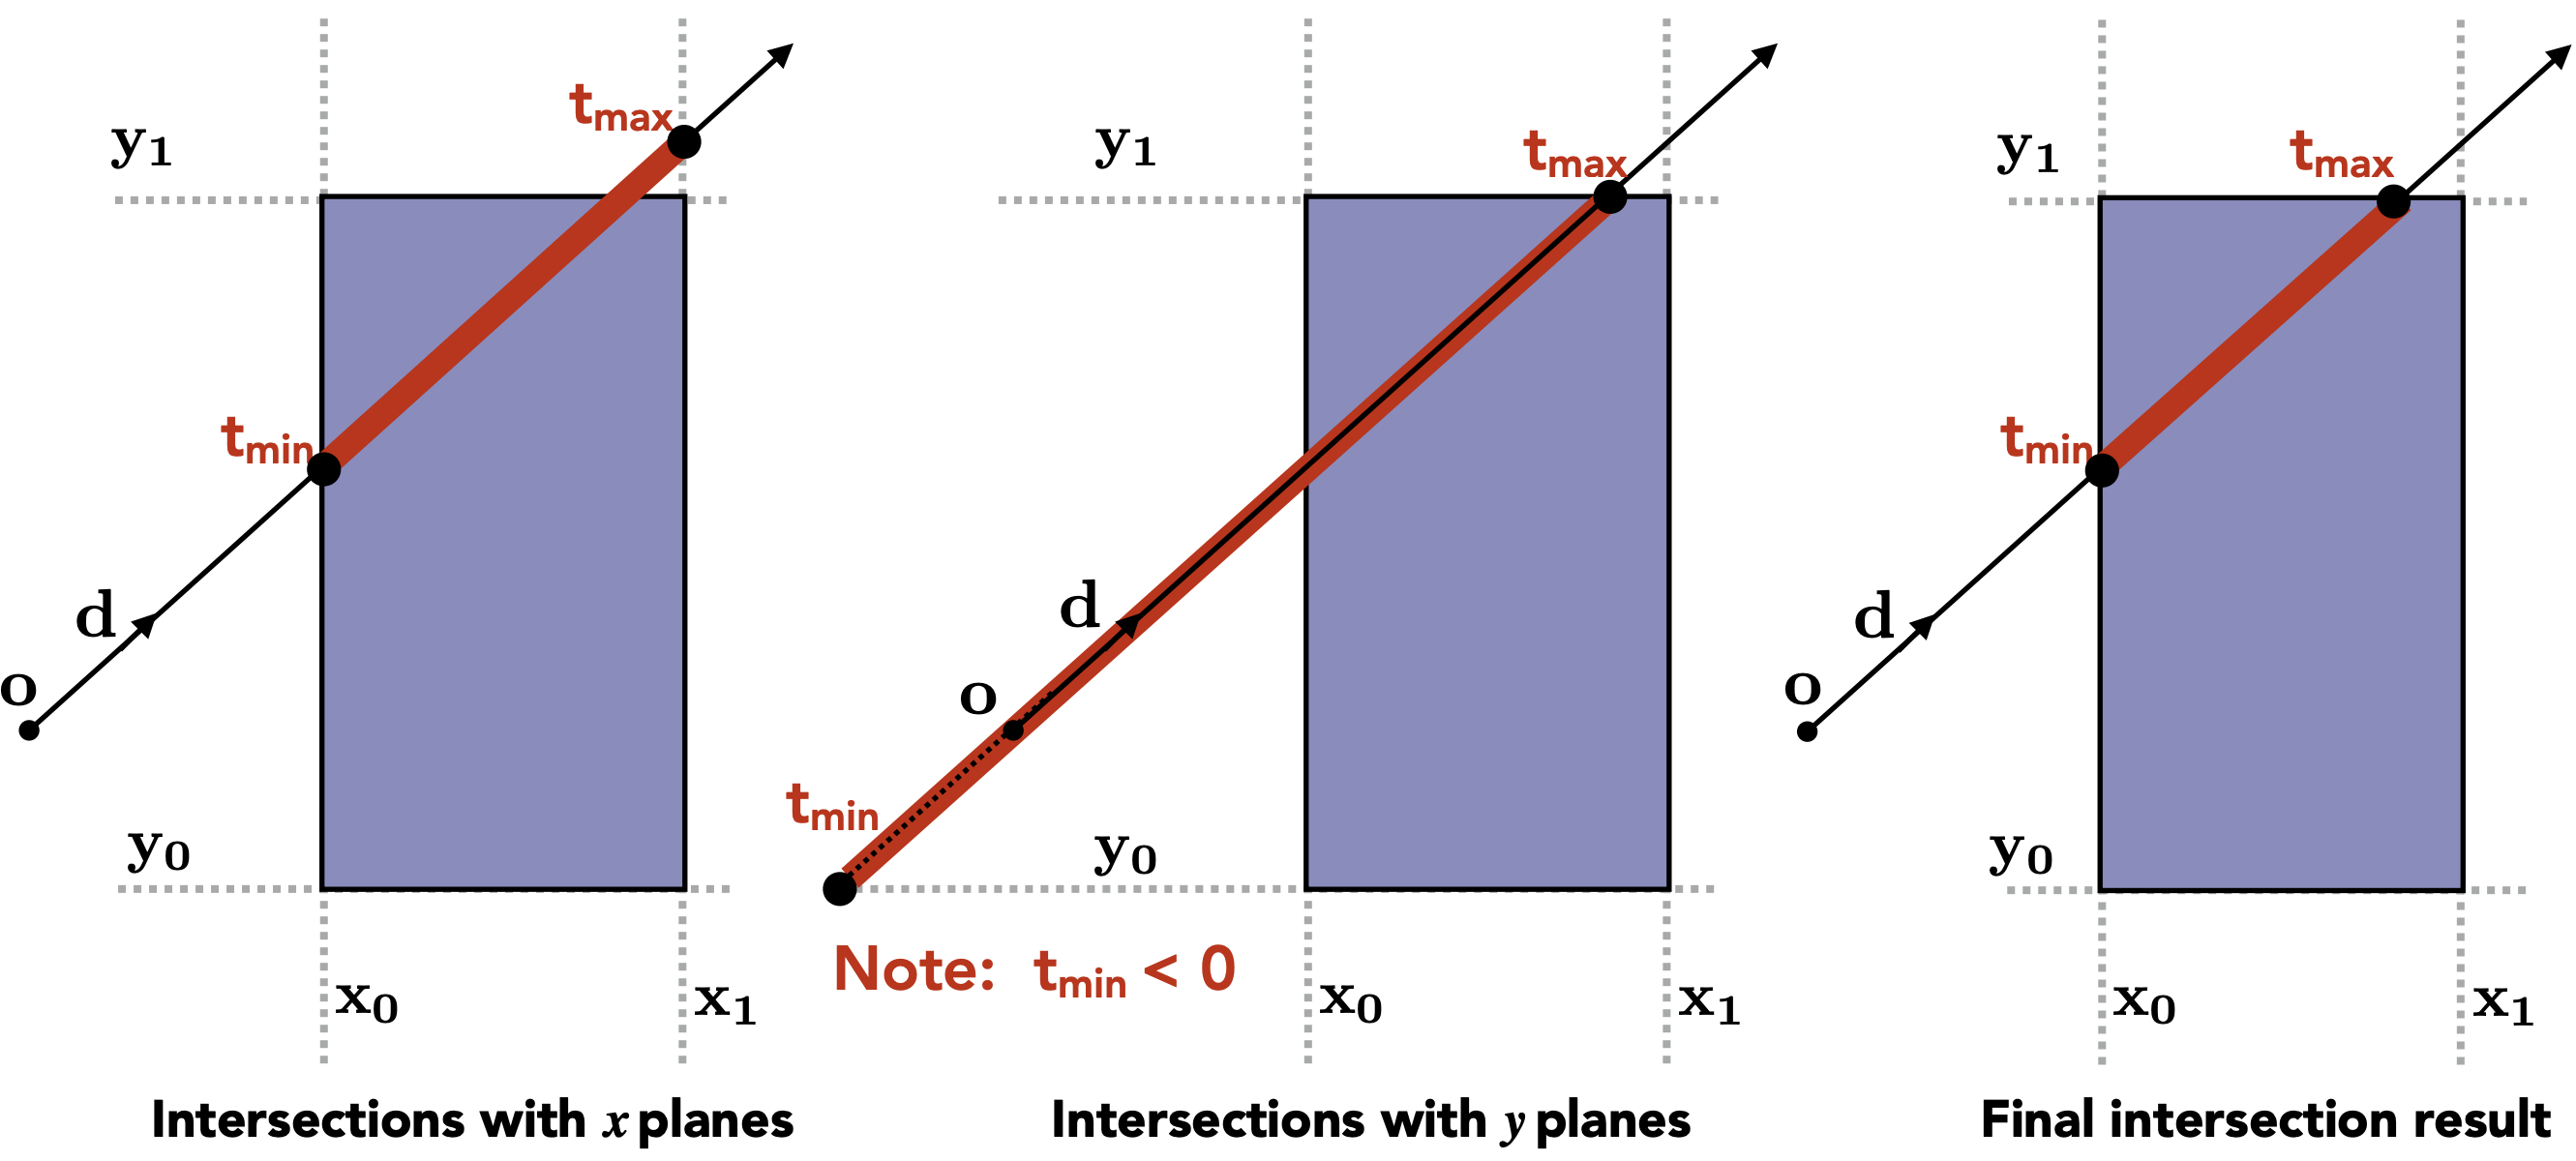
\includegraphics[scale=.25]{baoweitiji.png}
	\caption{包围体积中交点的计算}
	\label{fig:bwtj}
\end{figure}

我们求出光线在x平面上的两个交点以及y平面上的两个交点,那么最终光线在包围盒内部的部分是这些交点区间的交集。我们可以认为:
\begin{itemize}
	\item 光线进入到三个面中,才可以进入到包围盒;
	\item 光线离开任意一个面,就会离开包围盒。
\end{itemize}
我们对三对面分别求出进入时间$t_{min}$和离开时间$t_{max}$,那么最终对于包围盒来说进入时间$t_{enter}$是所有进入时间的最大值,离开时间$t_{exit}$是所有离开时间的最小值。如果进入时间小于离开时间,那么我们认为光线和盒子有交点。

对于时间出现负值的情况,我们进行以下讨论:
\begin{itemize}
	\item 如果离开时间$t_{exit}<0$,那么盒子在光线的背后,不会产生交点;
	\item 如果进入时间$t_{enter} < 0$,那么光线的起点在盒子的里面。
\end{itemize}

光线和盒子有交点,当且仅当(iff)$t_{enter}<t_{exit}, t_{exit}\geq 0$.
我们可以利用三角形相似性求出对应的$t$值。
\begin{figure}[H]
	\centering
	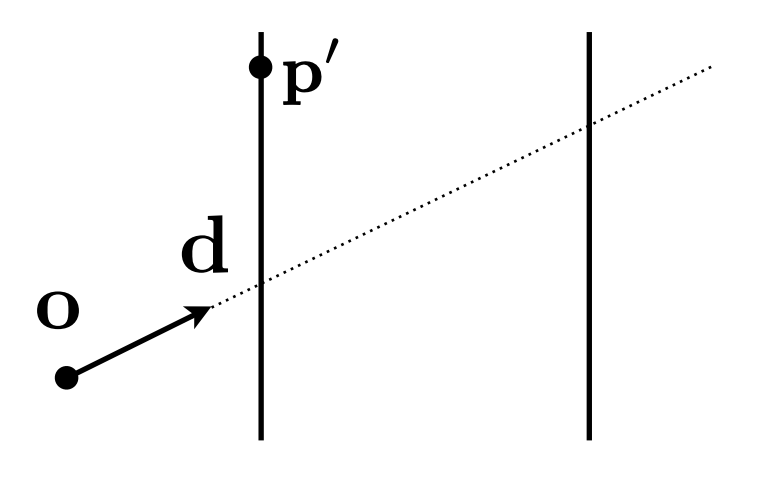
\includegraphics[scale=.25]{AABB.png}
	\caption{AABB中$t$值的计算}
	\label{fig:aabb}
\end{figure}
$t$值可以表示为:
\begin{equation}
	t=\frac{p'_x-o_x}{d_x}
\end{equation}

\subsection{空间划分}
为了可以加速光线和物体求交点,我们可以使用网格将原本比较大的包围盒进行划分。我们进行网格划分分为以下几个步骤:
\begin{enumerate}
	\item 找到场景中的包围盒;
	\item 将包围盒划分成一个一个小格子;
	\item 存储哪些小格子中包含物体(我们认为物体都是非实心的面,只记录包含面的小格子,物体内部不包含面的小格子不计入);
	\item 判断光线是否和格子相交,如果光线和某个格子相交并且这个格子中包含物体,那么我们需要与格子中的物体求光线的交点(这里有两个假设:1.判断光线和格子是否相交是很快的;2.我们可以使用计算机图形学中画直线的方法来判断哪些格子是会相交的。)。
\end{enumerate}
\begin{figure}[H]
	\centering
	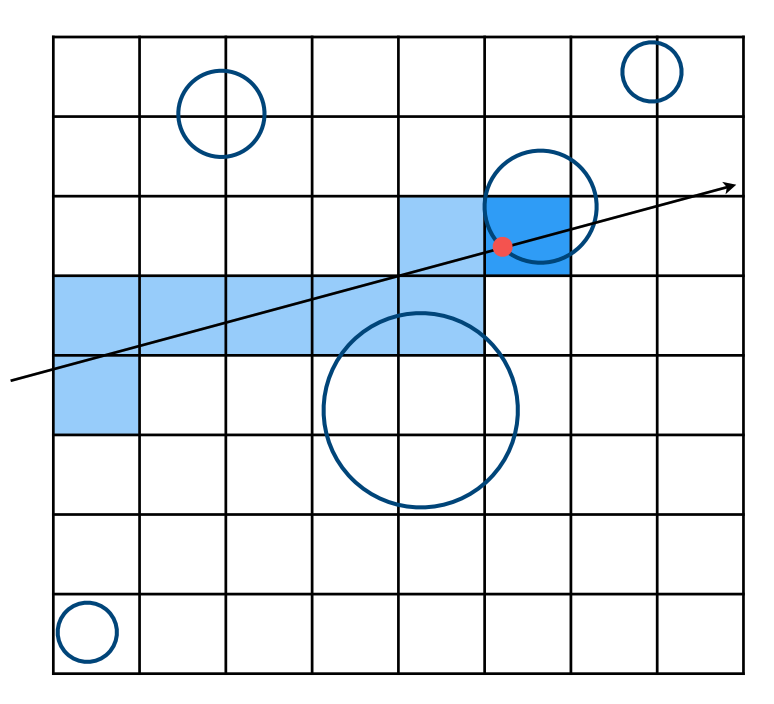
\includegraphics[scale=.15]{wanggehuafen.png}
	\caption{网格划分}
	\label{fig:wghf}
\end{figure}
一般来说,格子的划分不可以太稀疏也不可以太稠密,需要对格子的量进行控制。这种划分方式对于物体分布均匀的场景比较合适。对于物体分布稀疏的场景需要多次和格子进行相交判断,这种方法相对不合适。

我们会使用其他空间划分方法,包括八叉树(Oct-Tree),KD树(KD-Tree)以及BSP树(BSP-Tree)。
\begin{figure}[H]
	\centering
	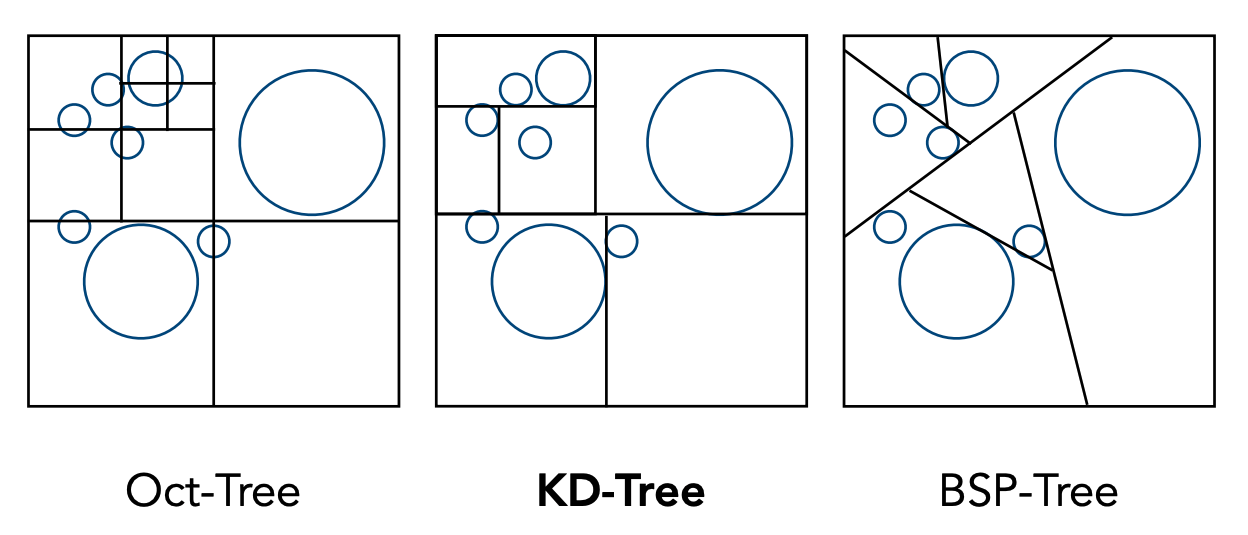
\includegraphics[scale=.15]{kongjianhuafen.png}
	\caption{空间划分}
	\label{fig:kjhf}
\end{figure}
\begin{itemize}
	\item \textbf{八叉树(Oct-Tree)},将一个包围盒切成八块(图中是二维情况,只有4块)。对于每一个小格子我们会继续进行划分直到小格子中没有物体或者物体的数量比较少;
	\item \textbf{KD树(KD-Tree)},每一次都进行一次水平划分或者竖直划分,将包围盒分成两部分。可以形成一个二叉树的存储结构。水平划分和竖直划分交替进行,保证划分的空间是均匀的;
	\item \textbf{BSP树(BSP-Tree)},每一次选择一个方向进行一次划分,并不是沿着轴平行方向划分。
\end{itemize}
三种划分方法,KD树更常用并且使用起来比较方便,可以用二叉树来存储。在每一个二叉树节点中,我们都要储存以下信息:
\begin{itemize}
	\item 如果是非叶子结点,需要存储划分轴,划分的位置以及孩子节点的指针;
	\item 如果是叶子结点,需要存储格子中包含的物体。
\end{itemize}

实际划分出的盒子均在叶子结点上。

\begin{figure}[H]
	\centering
	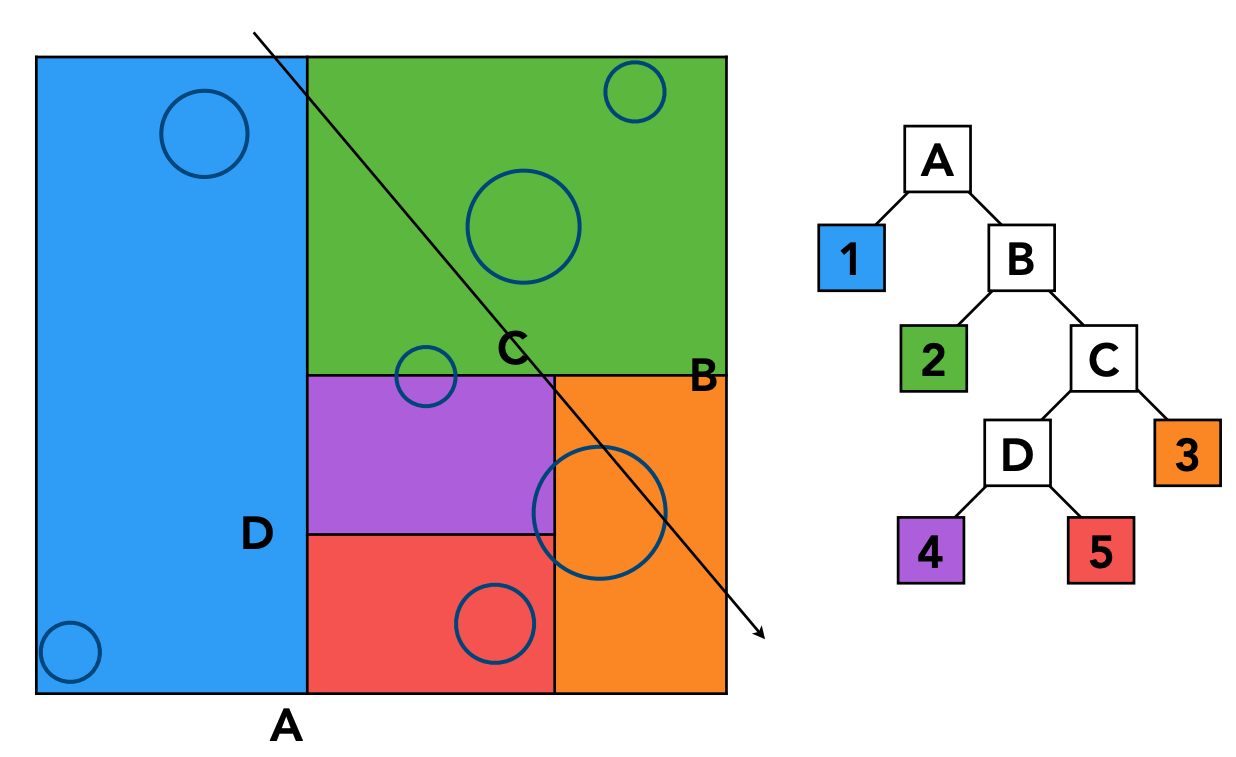
\includegraphics[scale=.15]{kongjianhuafenjisuan.png}
	\caption{空间划分后计算光线和物体的交点}
	\label{fig:kjhfjs}
\end{figure}
我们通过类似于二分查找的方式计算交点:
\begin{itemize}
	\item 如果光线和一个节点有交点,那么它和它的子节点也有交点;
	\item 如果光线和叶子结点有交点,那么它需要和格子内的所有物体求交点。
\end{itemize}
这种方法存在两个问题,首先,格子和一个三角形面是否相交的判断比较复杂。第二,一个物体可能会在多个不同的格子中,需要多次存储。因此我们会使用更常用的物体划分的方式。

\subsection{物体划分}
\textbf{物体划分(Bounding Volume Hierarchy,BVH)}的主要思想是对物体进行进行划分,并重新计算包围盒。BVH中,每一个物体只属于一个包围盒。BVH的划分主要分为三步:
\begin{enumerate}
	\item 划分包围盒;
	\item 递归的将包围盒划分为两部分;
	\item 当叶子结点的三角形面数量足够少的时候,停止划分。
\end{enumerate}
当我们进行划分的时候,也有不同的划分技巧:
\begin{itemize}
	\item 沿着最长的轴划分为两半(让长轴变短,分割更加均匀);
	\item 取中间的物体进行划分,可以保证两边三角形数量差不多(找到第k个物体的算法可以在$o(n)$的时间内解决,被称作快速选择算法);
	\item 当包围盒中的物体数量小于一定数量的时候停止划分。
\end{itemize}
使用伪代码可以写成如下形式:
\begin{lstlisting}[
	caption={BVH伪代码},
	language=c]
	Intersect(Ray ray, BVH node) {
		if (ray misses node.bbox) return;
		
		if (node is a leaf node)
			test intersection with all objs;
			return closest intersection;
		
		hit1 = Intersect(ray, node.child1);
		hit2 = Intersect(ray, node.child2);
		return the closer of hit1, hit2;
	}
\end{lstlisting}
这是一个递归算法。

\chapter{辐射度量学}
不论是光栅化还是光线追踪,都是对我们现实光照的近似表示。因此我们提出辐射度量学通过精准的物理定义模拟光照环境,使用更真实的方式进行光线追踪。辐射度量学描述了Radiant flux,intensity,irraddiance以及radiance。

\section{Radiant Energy and Flux}
\textbf{Radiant Energy}:指的是电磁辐射的能量。用符号$Q$表示,单位是焦耳$J$.

\textbf{Radiant Flux(Power)}:指的是单位时间的能量。$\Phi=\frac{dQ}{dt}$,单位是瓦特$W$,也可以用单位$lm$叫做流明(lumen)。是单位时间通过一个平面光照的量。

\section{Radiant Intensity}
\textbf{Radiant Intensity}指的是光源在单位立体角上的能量。数学定义为:
\begin{equation}
	I(\omega)=\frac{d\Phi}{d\omega}
\end{equation} 单位为$W/sr$或者坎德拉$candela=cd=\frac{lm}{sr}$.

\subsection{单位立体角}
在二维平面上,我们使用弧度制定义角度,定义为角度对应圆上的弧长除以半径:
\begin{equation}
	\theta = \frac{l}{r}
\end{equation} 单位是$rad$.整圆对应的角度为$2\pi\ rad$.

我们定义立体角为角度在球上对应的面积除以半径的平方:
\begin{equation}
	\omega=\frac{A}{r^2}
\end{equation} 单位是$sr$,整球对应的立体角为$4\pi\ sr$.

接下来我们推出\textbf{单位立体角(Differential Solid Angles)}的公式:
\begin{figure}[H]
	\centering
	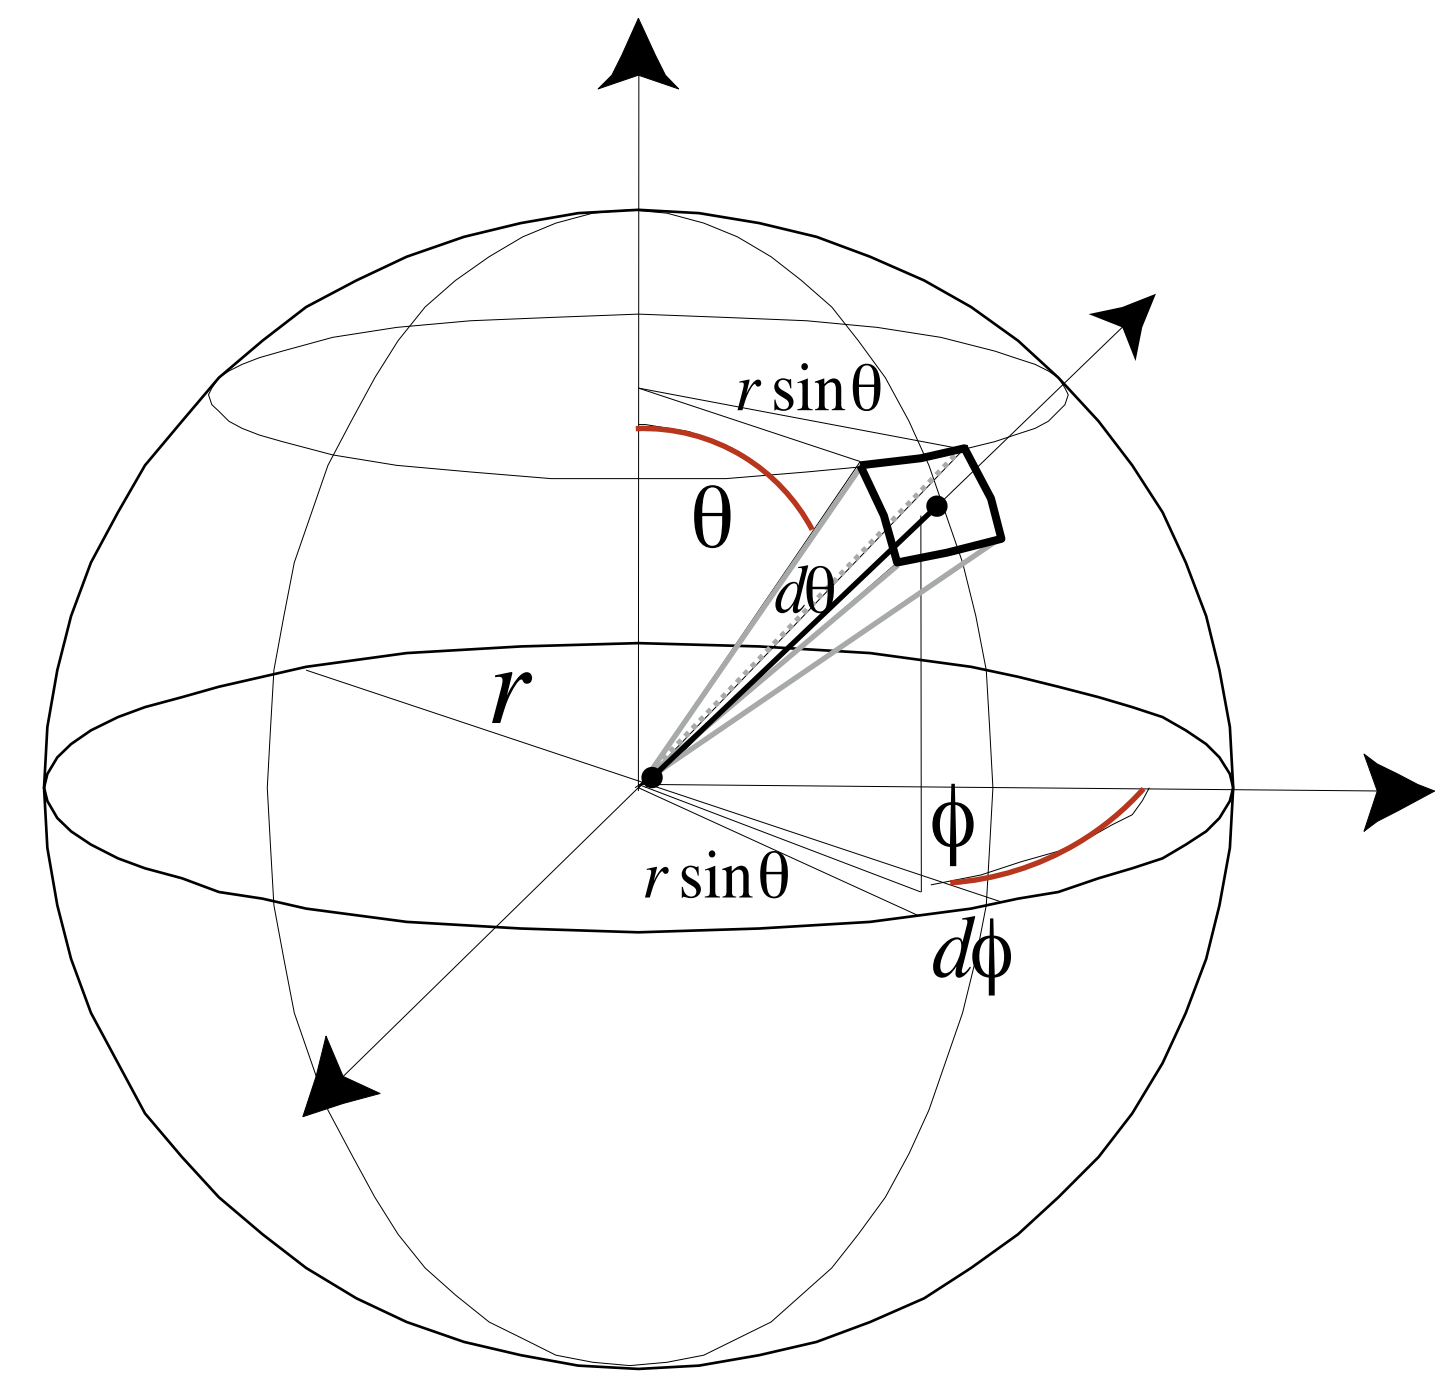
\includegraphics[scale=.25]{danweilitijiao.png}
	\caption{单位立体角推理}
	\label{fig:dwltj}
\end{figure}

\begin{equation}
\begin{split}
	dA=(rd\theta)(r\sin \theta d \phi)=r^2\sin\theta d\theta d\phi \\
	d\omega=\frac{dA}{r^2}=\sin\theta d\theta d\phi
\end{split}
\end{equation}

我们使用积分进行验证,对整个球面的单位立体角进行积分:
\begin{equation}
	\begin{split}
		\Omega=\int_{S^2}d\omega=\int_{0}^{2\pi}\int_{0}^{\pi}\sin\theta d\theta d\phi = 4\pi
	\end{split}
\end{equation}

因此,对于一个均匀发光的光源,$I=\frac{\Phi}{4\pi}$。

\section{Irradiance}

\textbf{Irradiance}指的是单位面积上所接收到的能量。定义为:
\begin{equation}
	E(x)=\frac{d\Phi(x)}{dA\cos\theta}
\end{equation} 单位是$W/m^2$或者$lux=\frac{lm}{m^2}$.接收到的能量应当是和平面垂直的光线带来的能量。如果光线和平面不垂直,我们需要将光线投影到平面的法线上,$\theta$是光线和平面法线的夹角。

我们回顾对于光能量衰减的理解,我们在Blinn-Phong模型中认为,点光源能量和距离成平方反比的关系。我们使用Irradiance来解释这个现象。我们认为任何一个球面上的Intensity不会发生衰减,之所以光的能量会发生衰减,正是因为相同的立体角下对应的球面面积增加,使得Irradiance发生变化。因此,点光源在某一个球面上的Irradiance和距离依然是平方反比关系。

\section{Radiance}
\textbf{Radiance}描述了光线的属性,它代表单位立体角单位面积上的能量。
\begin{figure}[H]
	\centering
	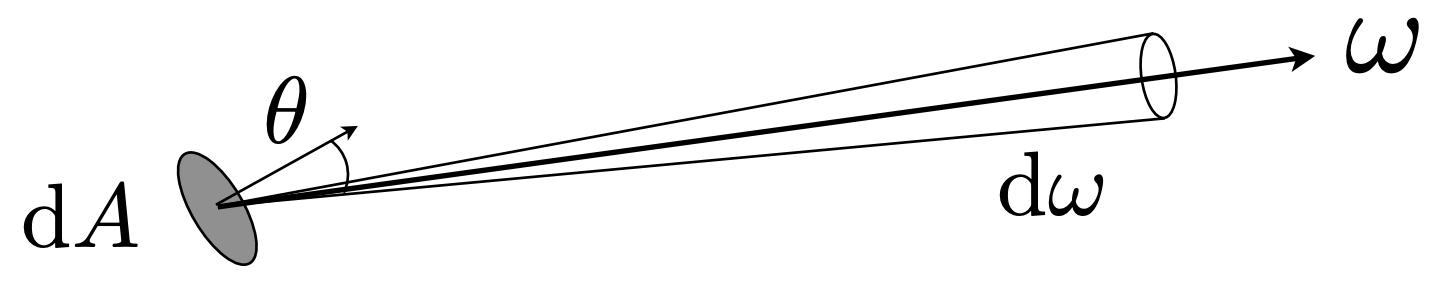
\includegraphics[scale=.25]{radiance.png}
	\caption{Radiance的计算}
	\label{fig:radiance}
\end{figure}

\begin{equation}
	L(p,\omega)=\frac{d^2\Phi(p,\omega)}{d\omega dA\cos\theta}
\end{equation} 单位是$W/(sr\cdot m^2)$或者$nit=\frac{lm}{sr\ m^2}=\frac{cd}{m^2}$.我们可以从两个方面来理解Radiance。从入射角度来说,我们认为Radiance是单位立体角下的Irradiance:
\begin{equation}
	L(p,\omega)=\frac{dE(p)}{d\omega \cos\theta}
\end{equation}

从出射的角度来说,我们认为Radiance是单位面积下的Intensity:
\begin{equation}
		L(p,\omega)=\frac{dI(p,\omega)}{dA \cos\theta}
\end{equation}

那么Irradiance也可以表示为Radiance在所有角度上的积分:
\begin{equation}
	\begin{split}
		dE(p,\omega)=L_i(p,\omega)\cos\theta d\omega\\
		E(p)=\int_{H^2}L_i(p,\omega)\cos\theta d\omega
	\end{split}
\end{equation}我们只对上半球做积分,我们认为和法线方向相反的光线对这一点没有贡献。

\section{双向反射分布函数}
\textbf{双向反射分布函数(Bidirectional Reflectance Distribution Fuction,BRDF)}定义了一个函数来表示从某一个角度入射的光线在某一个角度上会有多少能量被反射出去。我们将反射的过程理解为两步:第一步,光线入射物体得到了一部分能量;第二步,物体将得到的能量再一次射出去。

\begin{figure}[H]
	\centering
	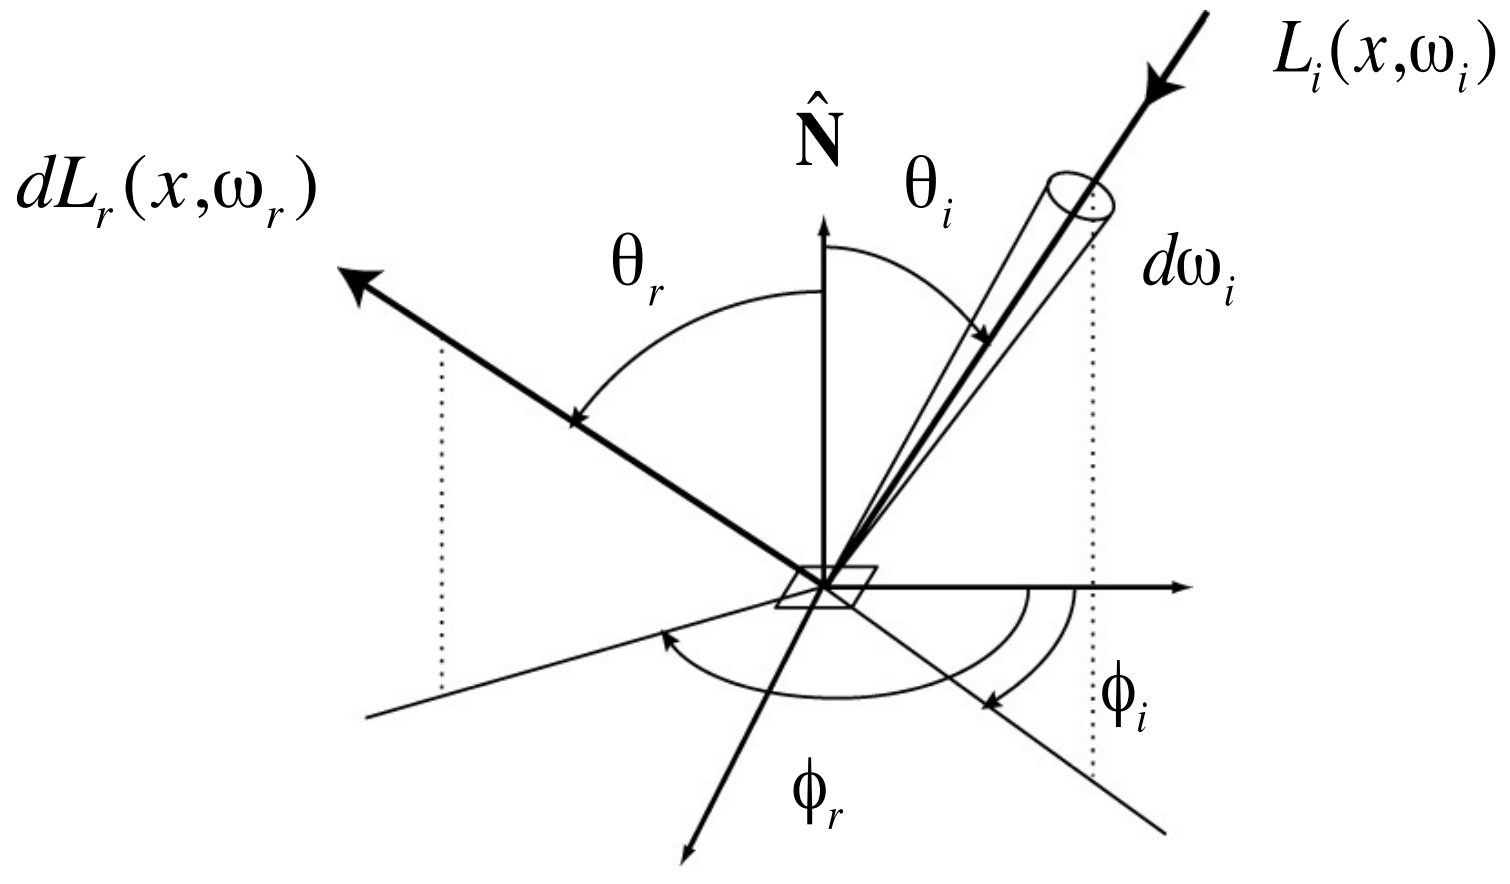
\includegraphics[scale=.25]{brdf.png}
	\caption{BRDF的定义}
	\label{fig:brdf}
\end{figure}

因此,我们定义双向反射分布函数为:
\begin{equation}
	f_r(\omega_i\rightarrow \omega_r)=\frac{dL_r(\omega_r)}{dE_i(\omega_i)}=\frac{dL_r(\omega_r)}{L_i(\omega_i)\cos\theta_i d\omega_i}[\frac{1}{sr}]
\end{equation}

那么,对于某一个出射方向,对应的能量应该是所有入射角度的光线反射结果的叠加:
\begin{equation}
	L_r(p,\omega_r)=\int_{H^2}f_r(\omega_i\rightarrow \omega_r)L_i(p,\omega_i)\cos\theta_id\omega_i
\end{equation}

一个物体除了会反射来自其他物体的光线之外,这个物体还有可能会自发光。因此,我们定义\textbf{渲染函数}为:
\begin{equation}
	L_o(p,\omega_o)=L_e(p,\omega_o)+\int_{\Omega^+}L_i(p,\omega_i)f_r(p,\omega_i,\omega_o)(n\cdot \omega_i)d\omega_i
\end{equation}渲染函数包含两部分,一部分是物体自发光,另一部分是反射光。在这里我们使用点乘代替$\cos\theta$计算。我们的积分区域只在上半球,法线反方向光线对于平面没有贡献。

我们再一次理解这个公式,我们可以认为$L_i$包含其他点光源,面光源以及其他物体二次反射光线。最终结果我们使用积分的方式进行叠加。那么这个公式可以简写为:
\begin{equation}
	I(u)=e(u)+\int I(v)K(d,v)dv
\end{equation} 我们可以通过矩阵再一次简化公式为:
\begin{equation}
	I=E+KL
\end{equation}
通过求解矩阵我们可以得到:
\begin{equation}
	L=(I-K)^{-1}E
\end{equation}

我们可以将矩阵进行展开,可以得到:
\begin{equation}
	\begin{split}
		L&=(1+K+K^2+K^3+\dots)E\\
		&=E+KE+K^2E+K^3E+\dots
	\end{split}
\end{equation}
每一项分别代表的是:物体直接发出的光,光源经过一次反射的光,光源经过两次反射得到的间接光照,……

\section{全局光照}
全局光照指的是直接光照以及间接光照的集合。光栅化处理的是0次项和1次项的部分,对于高阶项比较难处理。随着我们不断叠加不同反射次数的结果,图片会收敛到一个亮度,不会一直变亮

\chapter{蒙特卡洛路径追踪}

我们在上一节得到了渲染函数为
\begin{equation}
	L_o(p,\omega_o)=L_e(p,\omega_o)+\int_{\Omega^+}L_i(p,\omega_i)f_r(p,\omega_i,\omega_o)(n\cdot \omega_i)d\omega_i
\end{equation}
本节我们将通过数学工具求解这个函数并写成算法的形式来实现路径追踪。

\section{蒙特卡洛积分}

对于任意一个函数,不论是可以简单表达成解析式的还是不能轻松表达为解析式的函数,我们都希望求出其定积分的结果。在高等数学中我们使用\textbf{黎曼积分}求解。也就是我们将曲线下的面积近似成一系列的小长方形的和。当小长方形越多时,得到的结果越相近。

蒙特卡洛积分是通过多次随机采样并将采样对应的结果除以其概率密度的平均值作为积分结果。也就是说对于一个采样概率分布$X_i\sim p(x)$,蒙特卡洛积分为
\begin{equation}
	\int_a^b f(x) = F_N=\frac{1}{N}\sum_{i=1}^N\frac{f(X_i)}{p(X_i)}
\end{equation}

我们假设采样的概率分布是均匀分布,也就是说$X_i\sim p(x)=\frac{1}{b-a}$,那么蒙特卡洛积分可以表示为
\begin{equation}
	\int_a^b f(x) = F_N=\frac{b-a}{N}\sum_{i=1}^Nf(X_i)
\end{equation}

蒙特卡洛积分对于任何一种采样分布都是成立的。只要进行采样就可以得到对应的积分。使用蒙特卡洛积分要注意两点:
\begin{enumerate}
	\item 采样的次数越多,得到的结果越准确;
	\item 采样必须在积分域上进行采样。
\end{enumerate}

\section{路径追踪}
在之前的课程中我们介绍了Whitted-Style光线追踪,但是这种追踪方式具有其极限性。Whitted-Style光线追踪仅计算光线的镜面反射,因此对于某些弱于镜面反射的光线反射现象(这里称作Glossy)不能进行很好的表示。因此我们选择使用渲染方程得到更加准确的求解。

对于渲染函数我们有两个问题需要解决:
\begin{enumerate}
	\item 我们需要求解积分项;
	\item 这是一个递归的函数。
\end{enumerate}

\subsection{积分求解}

使用蒙特卡洛积分求解积分项。在这里我们限定仅计算来自光源的光线,如果是来自其他物体的光线,这里我们看作0.

我们和蒙塔卡洛积分进行对照,发现$f(x)$对应的是$L_i(p,\omega_i)f_r(p,\omega_i,\omega_o)(n\cdot \omega_i)$。积分域是$\omega_i$,$\omega_i$在上半球均匀分布采样的概率密度为$\frac{1}{2\pi}$。

因此渲染函数的积分项可以写成:
\begin{equation}
	\begin{split}
		L_o(p,\omega_o)&=\int_{\Omega^+}L_i(p,\omega_i)f_r(p,\omega_i,\omega_o)(n\cdot \omega_i)d\omega_i\\
		&\approx \frac{1}{N}\sum_{i=1}^{N}\frac{L_i(p,\omega_i)f_r(p,\omega_i,\omega_o)(n\cdot \omega_i)}{p(\omega_i)}
	\end{split}
\end{equation}

这样的过程我们可以写成伪代码的形式:
\begin{lstlisting}[caption=渲染函数积分项对光源光线求解伪代码]
shade(p, wo)
	Randomly choose N directions wi~pdf
	Lo = 0.0
	For each wi
		Trace a ray r(p, wi)
		If ray r hit the light
			Lo += (1 / N) * L_i * f_r * cosine / pdf(wi)
	Return Lo
\end{lstlisting}

对于间接光照,对于下图中的P点,如果我们想要求出来自Q点的光线,我们可以看作我们从P点看向Q点来自光源的光线反射得到的结果。那么以上的伪代码我们可以改写为递归的形式:


\begin{figure}[H]
	\centering
	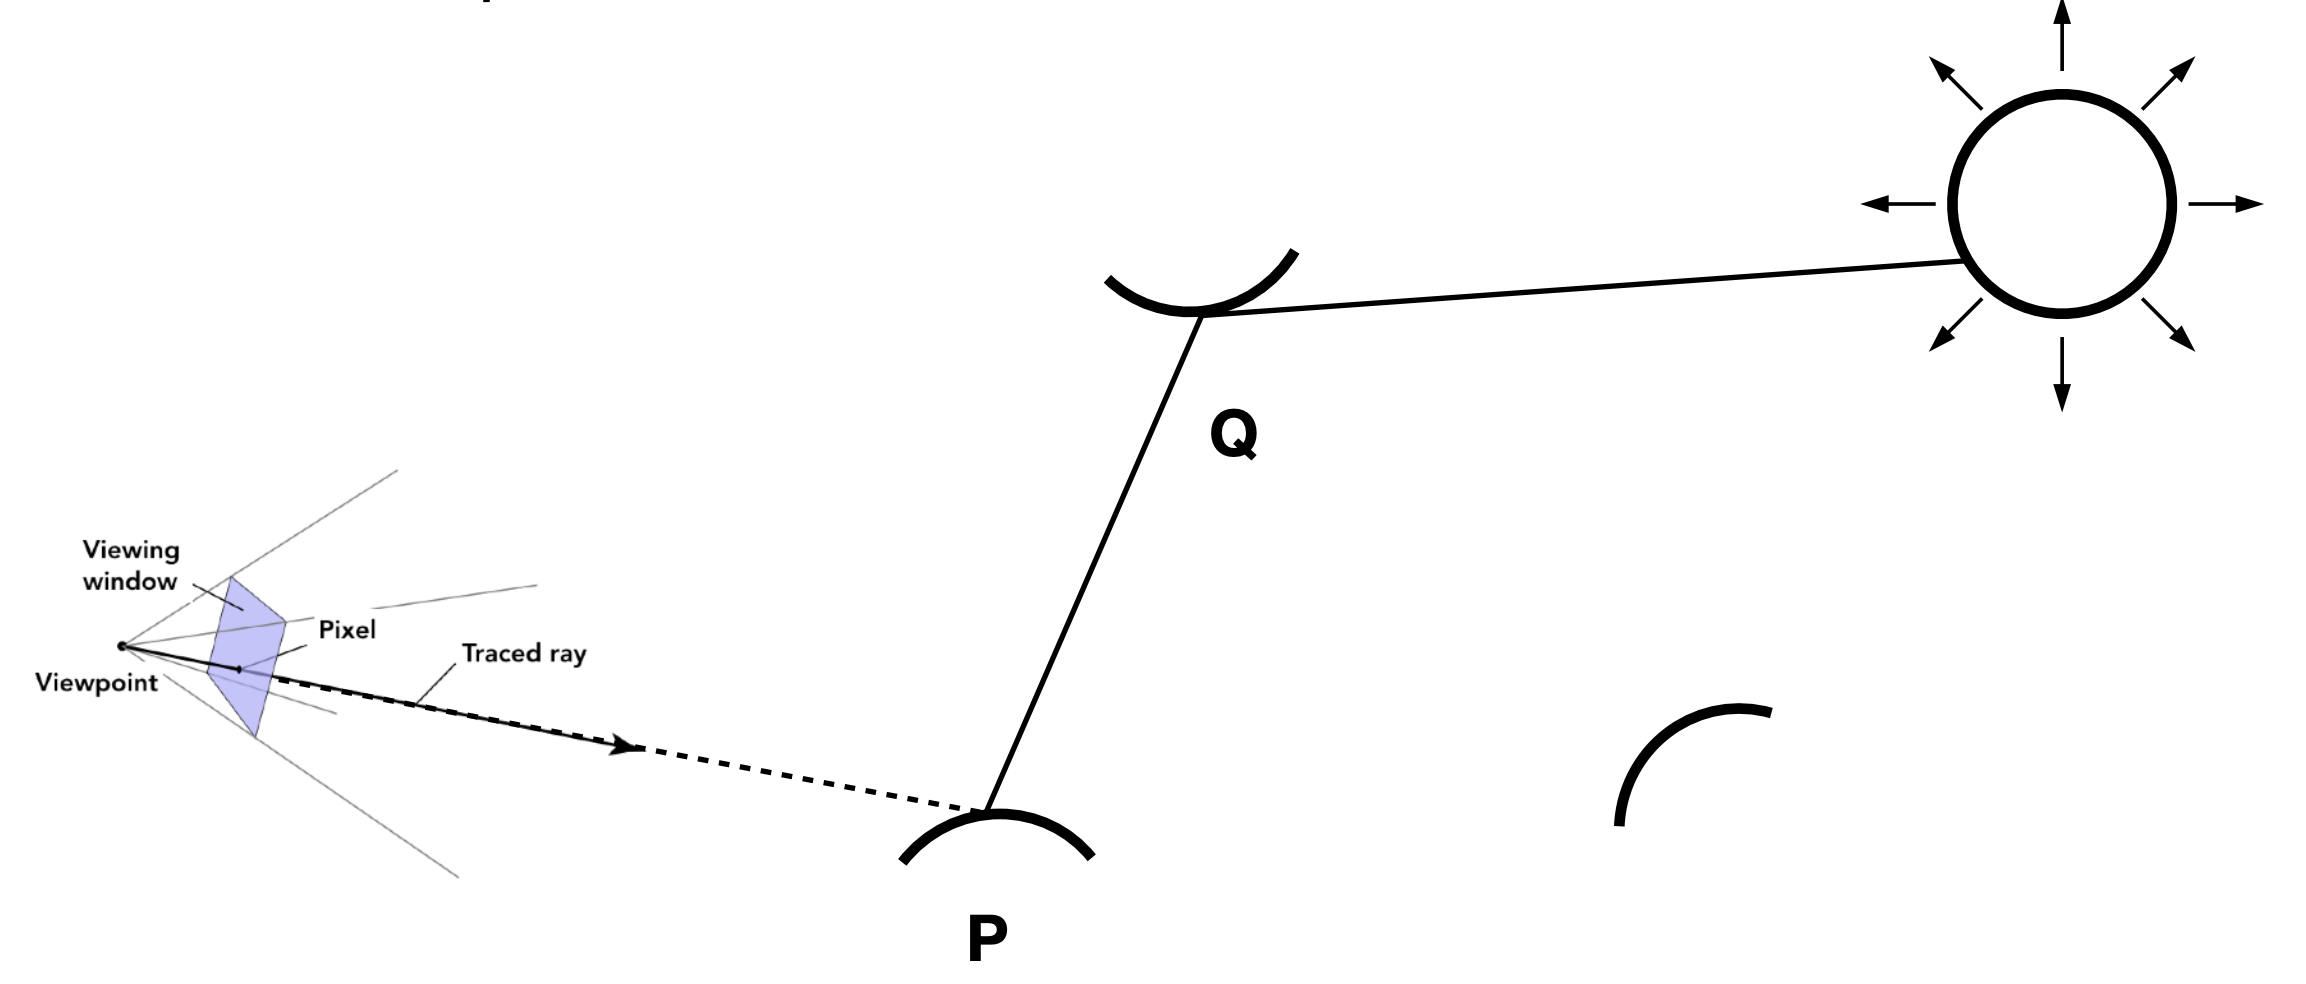
\includegraphics[scale=.25]{jianjieguangzhao.png}
	\caption{间接光照的递归求解}
	\label{fig:jjgz}
\end{figure}

\begin{lstlisting}[caption=渲染函数积分项的递归求解伪代码]
shade(p, wo)
	Randomly choose N directions wi~pdf
	Lo = 0.0
	For each wi
		Trace a ray r(p, wi)
		If ray r hit the light
			Lo += (1 / N) * L_i * f_r * cosine / pdf(wi)
		Else If ray r hit an object at q
			Lo += (1 / N) * shade(q, -wi) * f_r * cosine / pdf(wi)
	Return Lo
\end{lstlisting}

\subsection{算法优化}

\subsubsection{指数爆炸问题}

如果我们采样$N$次,那么在经过$r$次反射后,光线的数目可以达到$N^r$条,会使计算量大大增加。当且仅当$N=1$的时候,不会产生指数爆炸问题。此时我们转变方法,在计算积分的时候我们仅计1次,但是我们会在同一个像素中多次采样。也就是说,同一个像素上应该有多条光线通过,我们对这些光线分别计算渲染函数后求平均就是这一像素的结果。这个方法就是\textbf{路径追踪(Path Tracing)}。

\begin{lstlisting}[caption=渲染函数解决指数爆炸伪代码]
ray_generation(camPos, pixel)
	Uniformly choose N sample positions within the pixel
	pixel_radiance = 0.0
	For each sample in the pixel
		Shoot a ray r(camPos, cam_to_sample)
		If ray r hit the scene at p
			pixel_radiance += 1 / N * shade(p, sample_to_cam)
	Return pixel_radiance
\end{lstlisting}

\subsubsection{递归的停止问题}
我们的算法使用到了递归的方式。但是我们的算法没有递归的结束条件。因此我们需要引入一种方式结束递归。我们引入俄罗斯轮盘赌(RR)的方式。每一次光线都有$p$的概率能够反射出来。如果说光线可以反射,那么继续计算。反之直接返回0.那么伪代码的形式是:

\begin{lstlisting}[caption=包含递归停止条件的渲染函数伪代码]
shade(p, wo)
	Manually specify a probability P_RR
	Randomly select ksi in a uniform dist. in [0, 1]
	If (ksi > P_RR) return 0.0;
	 
	Randomly choose ONE directions wi~pdf
	Trace a ray r(p, wi)
	If ray r hit the light
		Return (1 / N) * L_i * f_r * cosine / pdf(wi) / P_RR
	Else If ray r hit an object at q
		Return (1 / N) * shade(q, -wi) * f_r * cosine / pdf(wi) / P_RR
\end{lstlisting}

我们返回的结果最终都会除以概率$p$,这样子,这一点得到结果的期望值和原来一样。每一条光线反射次数的期望值是$\frac{p}{(1-p)^2}$.

\subsubsection{均匀分布并非最优解}

对于同一个点来说,光源面积大,那么我们使用较少的光线就可以接触到光源。但是如果光源面积太小,我们必须使用较多的光线才可以和光源发生接触。那么对于小光源计算量会上升。因此我们希望使用其他的概率分布进行采样,使得采样得到的光线基本上都在光源上。

我们的解决方案是在光源上进行均匀分布的采样,这样子所有的光线一定都是来自于光源的。

\begin{figure}[H]
	\centering
	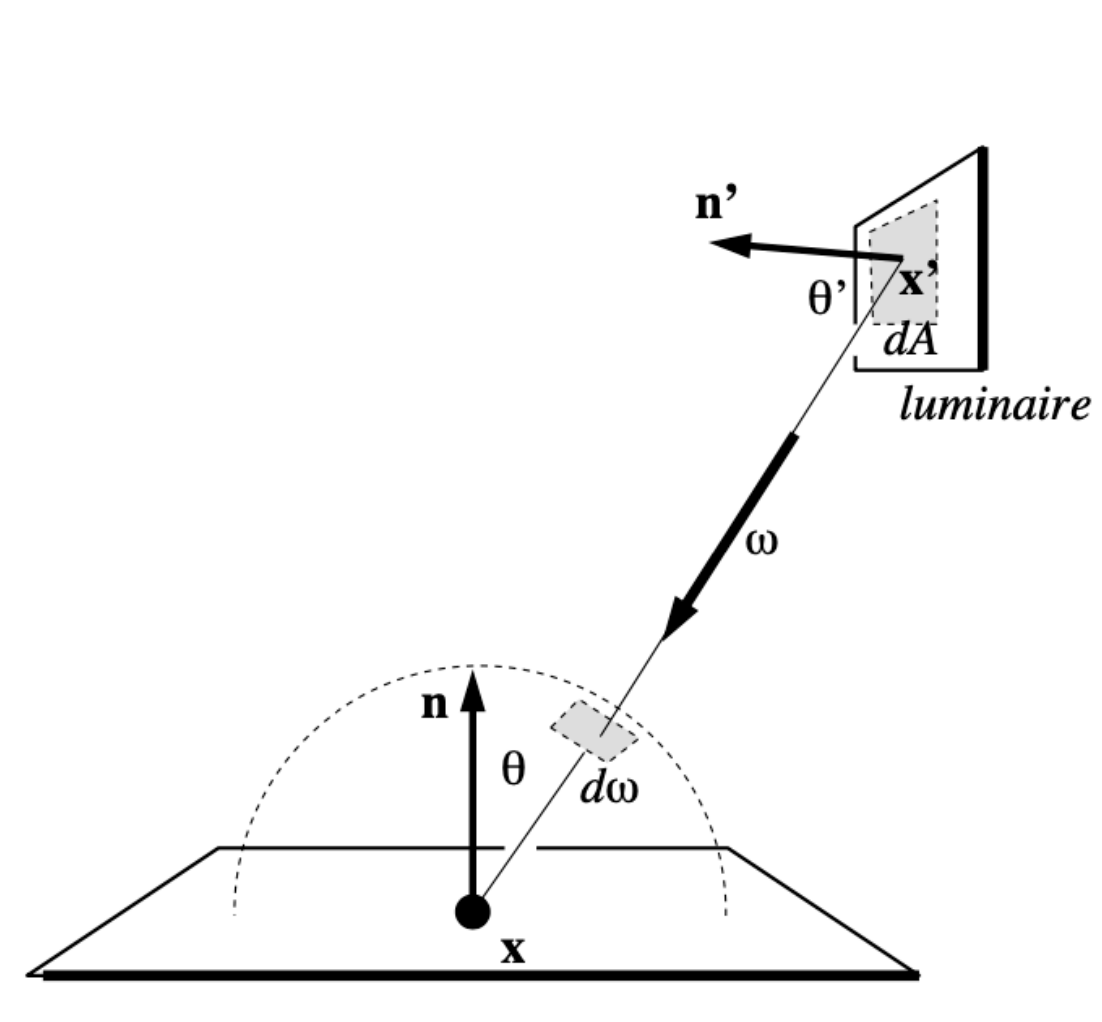
\includegraphics[scale=.25]{samplelight.png}
	\caption{从光源进行采样}
	\label{fig:samplelight}
\end{figure}

我们光源$A$上进行采样,那么概率密度应该是$\frac{1}{A}$。但是蒙特卡洛积分的采样必须在积分域上。此时积分域发生了变换,我们需要找到$d\omega$和$dA$之间的关系。$d\omega$是$dA$在对应单位球上的投影,因此
\begin{equation}
	d\omega = \frac{dA\cos\theta'}{||x'-x||^2}
\end{equation}

那么积分式就可以改变为:
\begin{equation}
	\begin{split}
		L_o(p,\omega_o)&=\int_{\Omega^+}L_i(p,\omega_i)f_r(p,\omega_i,\omega_o)\cos\theta d\omega_i\\
		&=\int_AL_i(p,\omega_i)f_r(p,\omega_i,\omega_o)\frac{\cos\theta\cos\theta'}{||x'-x||^2}dA
	\end{split}
\end{equation}

此时,我们需要更改一下之前RR的策略。对于直接光照,不使用RR;对于间接光照使用RR。这样我们就把问题分为了两部分——直接光照和间接光照。

\begin{lstlisting}[caption=采用光源上均匀分布渲染函数伪代码]
shade(p, wo)
	# Contribute from the light source
	Uniformly sample the light at x' (pdf_light = 1 / A)
	L_dir = L_i * f_r * cos(theta) * cos(theta') / |x' - p| ^ 2 / pdf_light
	
	# Contribute from other reflectors
	L_indir = 0.0
	Test Rassian Roulette with probability P_RR
	Uniformly sample the hemisphere toward wi (pdf_hemi = 1 / 2pi)
	Trace a ray r(P, wi)
	If ray r hit a non-emitting object at q
		L_indir = shade (q, -wi) * f_r * cos(theta) / pdf_hemi / P_RR
	
	Return L_dir + L_indir
\end{lstlisting}

最后我们只需要对光源和反射点间有物体的情况进行判断即可,

\begin{lstlisting}[caption=渲染函数伪代码]
	shade(p, wo)
	# Contribute from the light source
	L_dir = 0.0
	Uniformly sample the light at x' (pdf_light = 1 / A)
	Shoot a ray from p to x'
	If the ray is not blocked in the middle
		L_dir = L_i * f_r * cos(theta) * cos(theta') / |x' - p| ^ 2 / pdf_light
	
	# Contribute from other reflectors
	L_indir = 0.0
	Test Rassian Roulette with probability P_RR
	Uniformly sample the hemisphere toward wi (pdf_hemi = 1 / 2pi)
	Trace a ray r(P, wi)
	If ray r hit a non-emitting object at q
	L_indir = shade (q, -wi) * f_r * cos(theta) / pdf_hemi / P_RR
	
	Return L_dir + L_indir
\end{lstlisting}

这样我们就得到了最终路径追踪的算法。


\chapter{材质和外观}

\textbf{材质和外观(Material and Appearance)}是渲染物体非常重要的属性之一。光线的传播和材质具有密切的关系。

\section{材质的定义}

在渲染函数中,我们分析各个参数可以知道材质和双向反射分布函数(BRDF)具有密切的关系。BRDF决定了物体的材质属性。接下来我们将对三种不同的材质定义其对应的BRDF。

\begin{figure}[H]
	\centering
	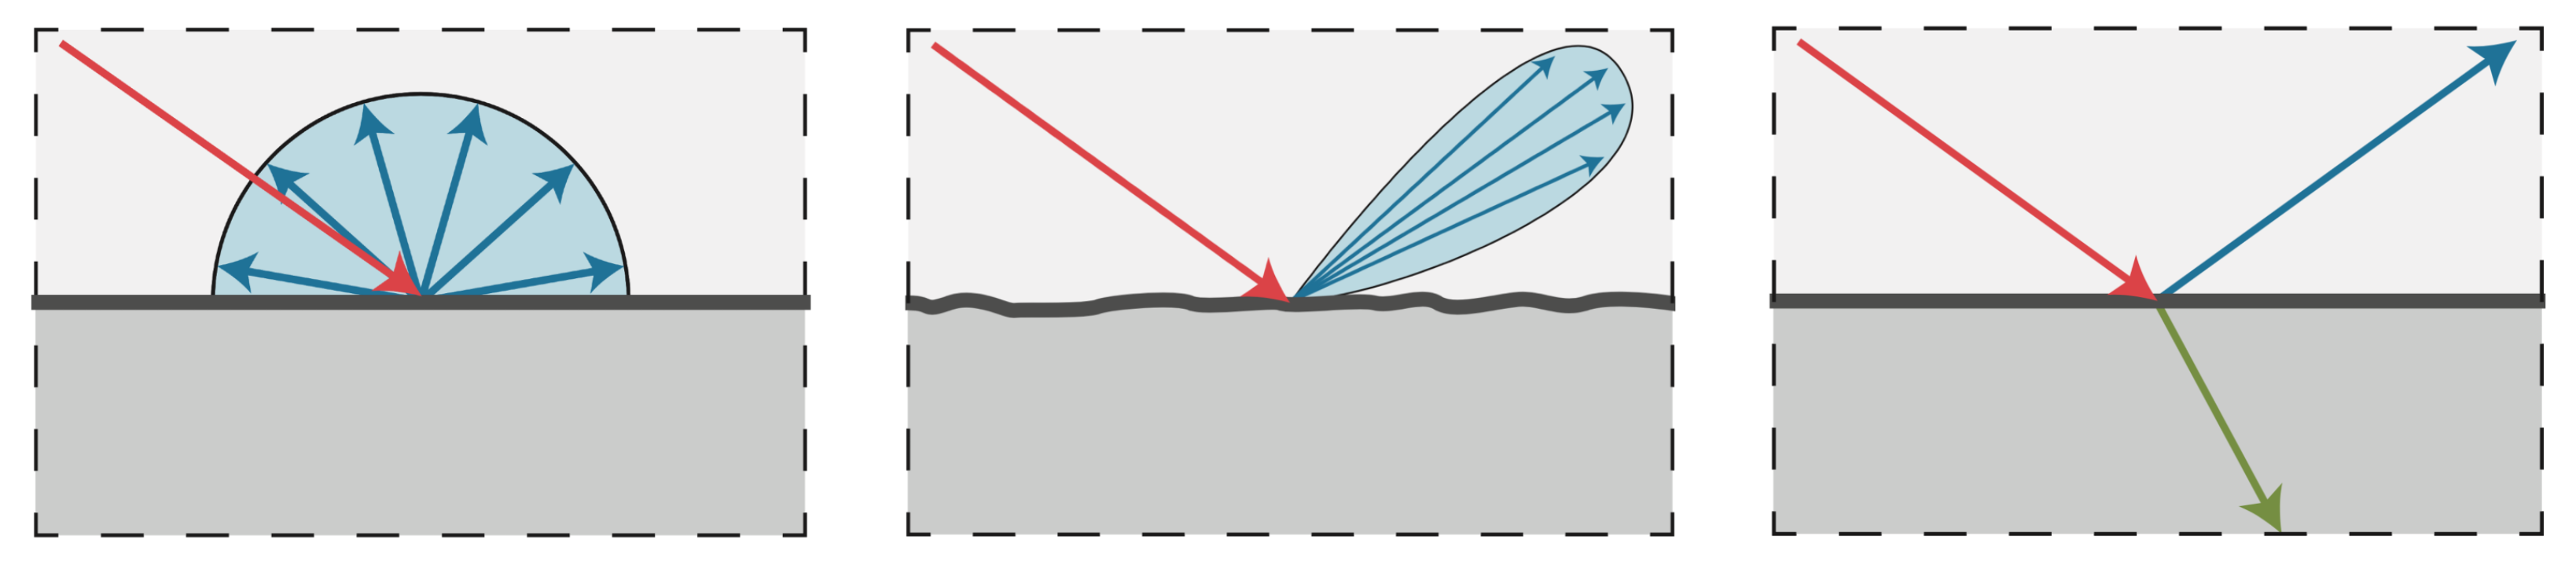
\includegraphics[scale=.35]{material.png}
	\caption{从左到右:漫反射材质,光泽表面材质以及折射材质}
	\label{fig:material}
\end{figure}

\subsection{漫反射材质}
\textbf{漫反射材质(Diffuse / Lambertian Material)}的性质是当一束光线从任意方向射向材质表面时,将会向各个方向均匀的反射光。

对于任何一个出射角$\omega_o$,对应的Radiance的大小为:
\begin{equation}
	\begin{split}
		L_o(\omega_o)&=\int_{H^2}f_rL(\omega_i)\cos\theta_id\omega_i\\
		&=f_rL_i\int_{H^2}cos\theta_id\omega_i\\
		&=\pi f_r Li
	\end{split}
\end{equation}
根据能量守恒定律,$L_o=L_i$,因此我们可以得到$f_r=\frac{1}{\pi}$。我们引入一个反射率(Albedo)$\rho$反应能量的衰减:
\begin{equation}
	f_r=\frac{\rho}{\pi}
\end{equation}
反射率既可以是一个通道对能量的衰减,也可以在RGB空间上定义一个三维的反射率来表示颜色。

\section{光泽表面材质和折射材质}

\textbf{光泽表面材质(Glossy material )}一般表示的是金属材质。这些材质相比于镜面来说没有那么光滑,但是依然可以产生非常类似于镜面反射的效果(光线的出射方向非常的集中)。

\textbf{折射材质(Ideal reflective / refractive material)} 可以折射一定量的光线。这种材质通常是透明材质,例如玻璃或者水。

\section{散射定律}

\subsection{反射定律}

\textbf{反射定律(Reflection Law)}指光射到一个界面上时,其入射光线与反射光线成相同角度。我们用数学方法定义在立体角上的反射定律:

\begin{figure}[H]
	\centering
	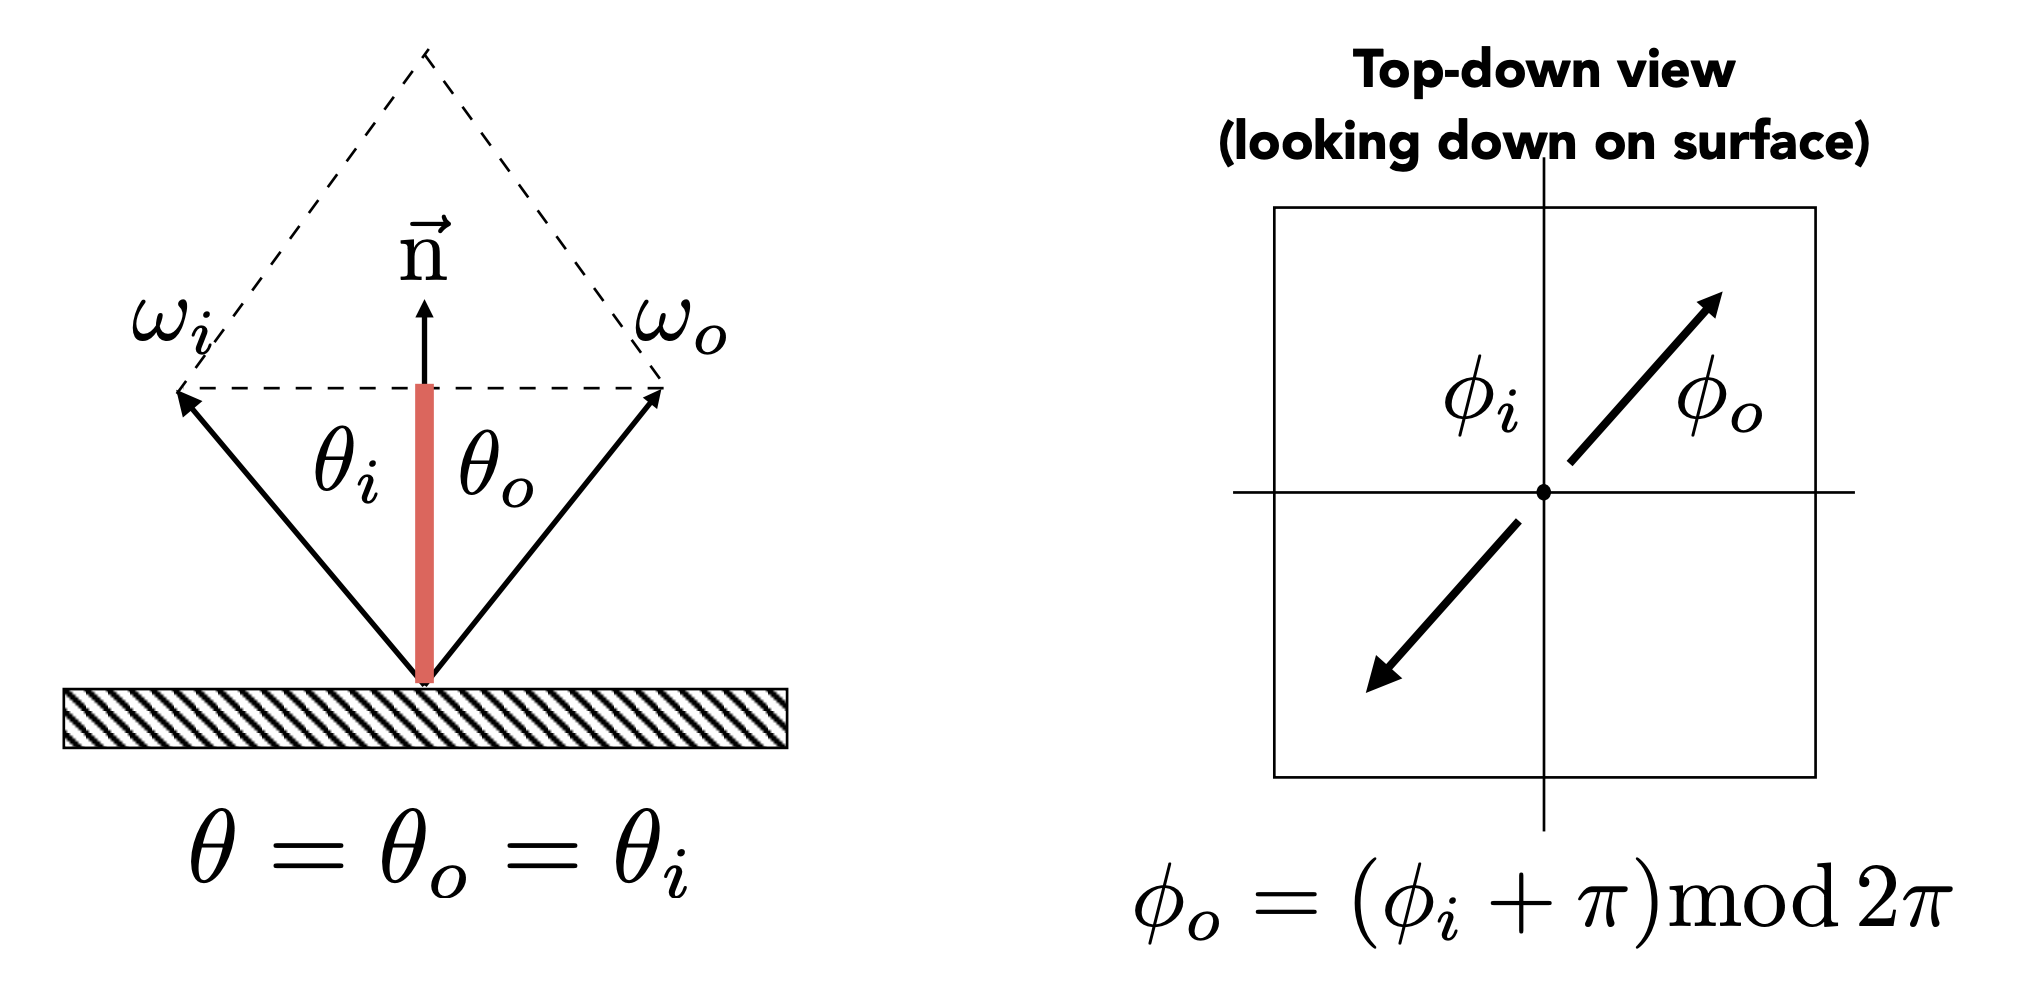
\includegraphics[scale=.25]{fanshe.png}
	\caption{反射定律}
	\label{fig:fanshed}
\end{figure}

在光线和法线所在的平面上,反射角等于入射角,也就是说$\theta=\theta_o=\theta_i$.如果我们垂直于法线观测,入射光线和反射光线方向完全相反,也就是$\phi_o=(\phi+\pi)\mod 2\pi$.

根据反射定律,我们在知道入射角和法线方向的时候就可以求出出射角方向:
\begin{equation}
	\begin{split}
		&\because \omega_o + \omega_i = 2\cos\theta \overrightarrow{n} = 2(\omega_i\cdot \overleftarrow{n})\overrightarrow{n}\\
		&\therefore \omega_o = -\omega_i + 2(\omega_i\cdot \overrightarrow{n})\overrightarrow{n}
	\end{split}
\end{equation}

\subsection{折射定律}

\textbf{折射定律(Snell's Law)}反映了折射角和入射角的关系。

\begin{figure}[H]
	\centering
	\includegraphics[scale=.25]{zheshe.png}
	\caption{折射定律}
	\label{fig:zheshe}
\end{figure}

根据折射定律,在光线和法线所在平面上,折射率和光线于法线的夹角正弦值相等。也就是说:
\begin{equation}
	\eta_i\sin\theta_i = \eta_t=\sin\theta_t
\end{equation}
其中$\eta$是这种材质的折射率。垂直于法线观测的情况和反射定律相同,两条光线方向是相反的。

常见的材质的折射率如下表所示:

\begin{table}[H]
	\centering
	\begin{tabular}{cl}
		\hline
		材质       & $\eta$  \\ \hline
		真空       & 1.0     \\
		空气(海平面)  & 1.00029 \\
		水(20摄氏度) & 1.333   \\
		玻璃       & 1.5-1.6 \\
		钻石       & 2.42  \\ \hline
	\end{tabular}
	\caption{常见材质的折射率}
\end{table}

根据折射定律,我们在知道入射角和法线方向以及材质的折射率的时候就可以求出出射角方向:
\begin{equation}
	\begin{split}
		\cos\theta_t&=\sqrt{1-\sin^2\theta_t}\\
		&=\sqrt{1-(\frac{\eta_i}{\eta_t})^2\sin^2\theta_i}\\
		&=\sqrt{1-(\frac{\eta_i}{\eta_t})^2(1-\cos^2\theta_i)}
	\end{split}
\end{equation}

我们对以上公式进行讨论。当根号下的结果如果小于0,当且仅当$\frac{\eta_i}{\eta_t}>1$.也就是说当入射介质的折射率大于反射介质的折射率时,就有可能发生\textbf{全反射}现象。

\section{菲涅耳项}

在现实生活中,我们发现这样的现象。当我们在不同的视角下进行观察的时候会用不同的现象。如下图所示,当我们从不同的视角观察桌子的时候,桌子对书反射的程度也不尽相同。这就是菲涅耳带来的结果。

\begin{figure}[H]
	\centering
	\includegraphics[scale=.25]{feinieer.png}
	\caption{菲涅耳项带来的现象}
	\label{fig:fne}
\end{figure}

对于导体和非导体,菲涅耳项满足:
\begin{itemize}
	\item 对于非导体,入射光线和入射平面越近,被反射出去的光线越多;
	\item 对于导体,反射出来光线的多少和入射角度没有直接关系,光线都可以被大量反射出去。
\end{itemize}

菲涅耳项的准确计算方法是:
\begin{equation}
	\begin{split}
		R_s&= \lvert\frac{n_1\cos\theta_i-n_2\cos\theta_t}{n_1\cos\theta_i+n_2\cos\theta_t}\rvert^2 = \lvert{\frac{n_1\cos\theta_i-n_2\sqrt{1-(\frac{n_1}{n_2}\sin\theta_i)^2}}{n_1\cos\theta_i+n_2\sqrt{1-(\frac{n_1}{n_2}\sin\theta_i)^2}}}\rvert^2\\
		R_p&= \lvert\frac{n_1\cos\theta_t-n_2\cos\theta_i}{n_1\cos\theta_t+n_2\cos\theta_i}\rvert^2 = \lvert{\frac{n_1\sqrt{1-(\frac{n_1}{n_2}\sin\theta_i)^2}-n_2\cos\theta_i}{n_1\sqrt{1-(\frac{n_1}{n_2}\sin\theta_i)^2+n_2\cos\theta_i}}}\rvert^2\\
		R_{eff}&=\frac{1}{2}(R_s+R_p)
	\end{split}
\end{equation}
其中,$R_s$和$R_p$是在s极点和p极点的菲涅耳项,我们使用他们的平均作为我们使用的菲涅耳项。但是这种计算方式过于的复杂,因此还提供了一种比较简单的菲涅耳项计算方法:
\begin{equation}
	\begin{split}
		R(\theta)&=R_0+(1-R_0)(1-\cos\theta)^5\\
		R_0&=(\frac{n_1-n_2}{n_1+n_2})^2
	\end{split}
\end{equation}

\section{微表面模型}

\textbf{微表面模型(Microfacet Material)}是更接近于物理的材质描述。我们认为\textbf{广表面(Macrosurface)}是平坦且粗糙的,但是\textbf{微表面(Microsurface)}是凹凸不平但是光滑的(每一个小的面都是光滑平坦的)。那么整体的光线反射情况应当是所有微表面反射情况的总和。从近处看是几何,从远处看就是一种材质。

对于任何一种材质,我们使用法线分布来描述其材质。如果是光滑的表面,那么法线分布比较集中;否则,法线会分布在四处。在微表面的情况下BDRF可以写作:
\begin{equation}
	f(i,o)=\frac{F(i,h)G(i,o,h)D(h)}{4(n,i)(n,o)}
\end{equation}
其中,$F(\cdot)$是菲涅耳项,$D(h)$是沿着半向量(Half Vector,$h=\frac{1}{2}(i+o)$)方向的法线分布。$G(\cdot)$是一个几何项,微表面内部可能会有几何遮挡,使一些微表面失去了作用。自遮挡容易发生在几乎和反射面平行入射的方向(Grazing angle)。分号下的两项是推倒项。

\section{材质的分类}

本节我们将材质根据法线的分布进行分类,分别是:
\begin{itemize}
	\item 各向同性材质(Isotropic Material):各个方向上法线分布一致的材质,满足$f_r(\theta_i,\phi_i;\theta_r,\phi_r)=f_r(\theta_i,\theta_r,\phi_r-\phi_i)$;
	\item 各向异性材质( Anisotropic Material):各个方向上法线分布不一致的材质,满足足$f_r(\theta_i,\phi_i;\theta_r-\phi_r)\neq f_r(\theta_i,\theta_r,\phi_r,-\phi_i)$,常见于打磨过的金属,尼龙材料。
\end{itemize}

\section{BRDF的性质}
\begin{itemize}
	\item 非负性
	\begin{equation}
		f_r(\omega_i\rightarrow \omega_o) \geq 0
	\end{equation}
	\item 线性可加
	\item 可逆性
	\begin{equation}
		f_r(\omega_i\rightarrow \omega_o)=f_r(\omega_o\rightarrow \omega_i)
	\end{equation}
	\item 能量守恒
	\begin{equation}
		\forall\omega_r\ \int_{H^2}f_r(\omega_i\rightarrow \omega_o)\cos\theta_id\omega_i\leq 1
	\end{equation}
	\item 各向同性材质的特别性质
	\begin{equation}
		f_r(\theta_i,\theta_r,\phi_r-\phi_i)=f_r(\theta_r,\theta_i,\phi_i-\phi_r)=f_r(\theta_i,\theta_r,|\phi_r-\phi_i|)
	\end{equation}
\end{itemize}

\section{BRDF的测量}

我们希望准确的测量出真实世界材质的BDRF。如下图所示,我们可以通过以下的实验方式测量某一种材质的BDRF。

\begin{figure}[H]
	\centering
	\includegraphics[scale=.25]{bdfrce.png}
	\caption{测量材质的BDRF}
	\label{fig:bdrfce}
\end{figure}

我们可以通过这样的装置得到各个入射方向和出射方向的BDRF,测量的算法如下:
\begin{lstlisting}[caption=BDRF的测量]
foreach outgoing direction wo
	move light to illuminate surface with a thin beam from wo
	for each incoming direction wi
		move sensor to be at direction wi from surface
		measure incident radiance
\end{lstlisting}

这样的测量方式是需要使用四维的参数。但是如果我们测量的是各向同性材质,参数可以降至三维。又因为可逆性,我们只需要测量一半的情况就可以。MERL BRDF Database就是一个包含了各种材质BRDF的数据库。

\chapter{高级渲染理论}

\section{高级光线传播(Advanced Light Transport)}

\subsection{有偏与无偏蒙特卡洛估计}

\textbf{有偏(Biased)}蒙特卡洛估计指的是如果我们取样后得到的估计值与要预测的真实值是有偏差的,那么我们认为这是一个有偏估计。当我们采样足够大的的时候,有偏估计也可以收敛到正确值,这说明了有偏估计具有一致性。\textbf{无偏(Unbiased)}蒙塔卡洛估计指的是不论我们选取多少样本进行估计,得到的期望值和正确值一样。

\subsection{双向路径追踪}

\textbf{双向路径追踪(Bidirectional Path Tracing,BDPT)}指的是我们分别从光源和眼睛(摄像机)引出半路径,并将半路径的终点连接起来形成路径。这种方法非常适用于光源出光线比较复杂的情况。但是实现困难并且渲染比较慢,是一种无偏的估计。

\begin{figure}[H]
	\centering
	\includegraphics[scale=.25]{bdpt.png}
	\caption{双向路径追踪}
	\label{fig:bdpt}
\end{figure}

\subsection{Metropolis 光线传播}

\textbf{Metropolis光线传播(Metropolis Light Transport,MLT)}使用马尔可夫链的方法进行采样。这种采样方式可以很容易的采样到某一个采样的临近点。其主要思想是,当一条路径可以到达光源时,那么临近的采样也应该容易到达光源。非常适用于困难场景的渲染,尤其是SDS(Specular-Diffuse-Specular)路径。但是很难估计收敛速度,每一个像素的收敛速度也不一样。操作独立,各个像素独立导致画面会比较``脏”,因此很难应用到动画上。同样,这可以无偏估计。

\subsection{光子映射}

\textbf{光子映射(Photon Mapping)}是一个分为两步的方法。是一种有偏估计。适合于SDS路径以及焦散材质。
\begin{enumerate}
	\item 从光源出发射出光子,当光子反射到漫反射平面时停止,记录光子位置;
	\item 从摄像机射出半路径,直到路径反射到漫反射平面上。
\end{enumerate}

我们需要通过局部密度估计在计算单位面积内,光子数的多少。那么光子密度越高的地方应当越亮。对于任意一个点,我们选取临近$N$个距离最近的光子,那么使用$N$处以光子所占的面积$\triangle A$就可以得到该点的局部密度。

\begin{figure}[H]
	\centering
	\includegraphics[scale=.25]{mlt.png}
	\caption{光子的局部密度估计}
	\label{fig:mlt}
\end{figure}

为什么这是一个有偏的方法?我们$N$太少的话易产生噪声,但是$N$太多又会模糊。当我们使用的光子足够多的时候,$\triangle A$就趋近于$\text{d}A$.因此,只要我们的采样是有限的,得到的密度多少都会有偏差,所以这是一个有偏的估计。但是这是一致的估计。

\subsection{VCM}

\textbf{Vertex Connection and Merging (VCM)}是一种结合了双向路径追踪和光子映射的方法。其主要思想是在双向光线追踪中如果半路径的结束点并不在一起但是距离比较近的话可以组合在一起。使用光子映射的方法来组合这些临近的``光子”。是一种有偏估计。

\subsection{实时辐射度}

\textbf{实时辐射度(Instant Radiosity,IR)}最主要的思想是认为被照亮的表面可以当作一个小光源。从光源打出来的地方到一些表面后,到达点就是新的虚拟光源。之后就可以将这些虚拟光源看作光源进行渲染。优点是渲染速度快并且在漫反射场景中表现的很好。缺点是不能很好的处理反射材质。

\section{高级外观建模}

\subsection{非表面模型}

\subsubsection{散射介质}

对于一些\textbf{散射介质(Participating media)},例如云、雾,我们认为他们是非表面模型。因此他们不存在一个表面,而是由许多散射小颗粒组成的。任何一束光通过散射介质,会发生(部分)吸收或者散射。

\begin{figure}[H]
	\centering
	\includegraphics[scale=.35]{pm.png}
	\caption{散射介质的吸收,发光,外散射和内散射}
	\label{fig:pm}
\end{figure}

我们采用相位函数去描述在某一点光的散射和散射角度的关系。

\begin{figure}[H]
	\centering
	\includegraphics[scale=.35]{phasefunction.png}
	\caption{相位函数}
	\label{fig:pf}
\end{figure}

在渲染时我们会随机选择一个方向进行弹射,随机选择一个方向直接进行传播,在每一个点上和光线相连。

\subsubsection{毛发}

光线和头发的作用不是简单的光线和表面的作用。首先,我们将头发看作一个圆柱体。在Kajiya-Kay模型中,我们认为一束光射到头发上后,头发可以将光线散射成一个圆锥。但是这种模型渲染出来的效果不好。

\begin{figure}[H]
	\centering
	\includegraphics[scale=.15]{kkmodel.png}
	\caption{Kajiya-Kay模型}
	\label{fig:kk}
\end{figure}

Marschner模型认为,头发是一个能够透光的``玻璃”,因此光线应该分为三部分,分别是:
\begin{itemize}
	\item R:光线直接反射光;
	\item TT:光线经过两次折射后射出的折射光;
	\item TRT:光线折射后经过一次介质内反射后的折射光。
\end{itemize}

\begin{figure}[H]
	\centering
	\includegraphics[scale=.25]{mmodel.png}
	\caption{Marschner模型}
	\label{fig:mm}
\end{figure}

以上的模型对于人类的毛发已经有了很好的表现,但是对于动物毛发来说,表现并不好。这是因为动物的毛发并不是单层的结构。动物毛发中包含一层毛髓质(Medulla),因此引入双层模型(Double Cylinder Model)来对毛发进行建模。

\begin{figure}[H]
	\centering
	\includegraphics[scale=.25]{dcmodel.png}
	\caption{Double Cylinder模型}
	\label{fig:dc}
\end{figure}

在这个模型中我们额外增加了两种光:
\begin{itemize}
	\item TT$^s$:经过了中间介质的TT光线;
	\item TRT$^s$:经过了中间介质的TRT光线。
\end{itemize}

这样5种光线结合在一起得到的毛发会更加的真实。

\subsubsection{粒状材质}

\textbf{粒状材质(Granular Material)}是由细小的颗粒组成的材质,例如谷物,沙子,调味料等。这样的材质也有程序性的方法进行渲染。

\subsection{表面模型}

\subsubsection{半透明材质}

\textbf{半透明材质(Translucent Material)}指的是能够透光的一些材质,光线可以从一个地方进去并从另一个地方出去。例如玉石,水母都是典型的半透明材质。

由于一条光在半透明材质上入射后,出射光的起点并不一定在入射点上,因此我们需要对BRDF进行拓展。此时BDRF就变成了BSSDRF,此时我们需要引入新的位置参数,我们不仅要对角度进行积分,还要在面积上进行积分:
\begin{eqnarray}
	S(x_i,\omega_i,x_o,\omega_o)
\end{eqnarray}

\begin{eqnarray}
	L\left(x_{o}, \omega_{o}\right)=\int_{A} \int_{H^{2}} S\left(x_{i}, \omega_{i}, x_{o}, \omega_{o}\right) L_{i}\left(x_{i}, \omega_{i}\right) \cos \theta_{i} \mathrm{~d} \omega_{i} \mathrm{~d} A
\end{eqnarray}

我们会等效的认为,一个半透明材质上有一束光摄入相当于在介质的外部和内部各有一个光源。

\subsubsection{织物}

\textbf{织物(Cloth)}的制作工艺比较的复杂。首先,多层(Ply)缠绕会变成一根纱(Yarn),多根纱相互缠绕就会变成一根线(Fiber)。我们可以使用两种编织工艺,一种是机织(Woven),通过线之间的经纬交叉得到布料,另一种方式是手打(Knitted)的方式,类似于织毛衣的过程。

不同的布料有不同的BDRF,常见的渲染方法有:
\begin{itemize}
	\item 把布料看作非表面材质,将纤维划分为多个小方格进行渲染,每个小方格单独判断散射性质;
	\item 最暴力的做法是直接计算每一个纤维的结果。
\end{itemize}

当然,对于天鹅绒材质等布料,使用BDRF并不合适。

\subsection{真实世界模型}

我们认为现在的渲染器渲染出的画面并不真实,主要原因是这些渲染器过于完美。在实际生活中的物体一般表面都会带有划痕,会让物体表面看起来更真实。

我们可以用微表面模型的发现分布来解决这种情况。我们只需要在微表面模型的分布上加一些噪声,就可以产生带有划痕的效果。但是,在这样的法线分布下,光线很难反射到光源处。因此,我们的解决方案是,我们对于每一个像素,对应一部分法线分布$p-NDF$,使用这一部分的法线总体分布进行路径追踪。

此外,目前研究比较前沿的问题还有\textbf{波动光学(Wave Optics)}的渲染。

\section{程序化生成}

\textbf{程序化生成(Procedural Appearance)}指的是我们可以不定义一个纹理,而是直接定义一个噪声,通过噪声计算纹理。木纹,陶瓷都可以定制对应的纹理进行程序化的生成。

\part{其他知识}

\chapter{相机、镜头和光场}

\section{小孔成像}

用一个带有小孔的板遮挡在墙体与物之间,墙体上就会形成物的倒立的实像,我们把这样的一种现象叫\textbf{小孔成像(Pinhole Image Formation)}。小孔成像的特点是得到的成像没有景深效果。

除了小孔成像之外,我们还会使用透镜成像。之所以必须要使用小孔或者透镜是因为传感器上每个点需要记录对应方向光线的数据。如果不使用小孔或者透镜,那么到达传感器上的光线将来自各个方向,不能区分。

\section{视场}

摄像机的\textbf{视场(Field of View,FOV)}的大小和传感器的大小以及焦距(小孔成像中指的是传感器和小孔的距离)有关。

\begin{figure}[H]
	\centering
	\includegraphics[scale=.25]{fov.png}
	\caption{FOV}
	\label{fig:fov}
\end{figure}

根据相似三角形性质可知,
\begin{equation}
	\text{FOV}=2\arctan(\frac{h}{2f})
\end{equation}

\begin{itemize}
	\item 传感器越大,视场越大;
	\item 焦距越短,视场越大。
\end{itemize}

由于一些历史原因,在实际应用中,我们会采用35mm胶片($36\times 24 mm$)对应的焦距来反映视场的大小。焦距越小,对应的视场越大;焦距越大,拍摄的距离越远。较小的传感器需要使用较短的焦距来保持一样的视场。

\section{曝光}

\textbf{曝光(Exposure,$H$)}可以表示为曝光时间$T$和Irradiance $E$的乘积。
\begin{equation}
	H=T\times E
\end{equation}
其中,曝光时间由快门控制,Irradiance是单位时间传感器单位面积上接受的光的强度,由光圈和焦距控制。

\subsection{曝光控制}

曝光的控制由以下三个参数决定:
\begin{itemize}
	\item 光圈大小(Aperture Size):光圈的大小由f-stop控制,光圈是一个类似于瞳孔的结构。记做$FN$或者$F/N$,其中$N$是f数,计算方法是$f/D$,也就是焦距除以光圈的直径。光圈越大,景深效果越明显。
	\item 快门速度(Shutter Speed ):决定了传感器的感光时间;快门速度越慢,得到的图片会出现模糊,我们称作\textbf{运动模糊(Motion Blur)}。运动模糊会使图像变模糊,但是可以体现出运动速度快,符合人眼规律。对于某些包含快速旋转物体的图片,由于图像每一个部分都在不同时间拍摄,因此会出现\textbf{卷帘快门(Rolling Shutter)}的现象。
	\item ISO感光度(ISO Gain):传感器值乘一个常数变换为数字图像值,是一种后期处理。在数字相机中,高ISO会增加噪声。ISO是一种线性增长(ISO 200增加亮度的一半就是ISO 100)。
\end{itemize}

\begin{figure}[H]
	\centering
	\includegraphics[scale=.25]{expose.png}
	\caption{常见曝光参数的比较}
	\label{fig:expose}
\end{figure}

光圈和快门速度都可以控制曝光,因此理论上在一定的组合方式下,能够得到相同的曝光结果。但是,由于光圈和快门速度所带来的副作用不同,因此不同组合产生的效果也会有一些不同。在下表中,光圈和快门速度的组合能够得到相同的曝光。

\begin{table}[H]
	\centering
	\begin{tabular}{ccccccccccc}
		\hline
		f-stop & 1.4   & 2.0   & 2.8   & 4.0  & 5.6  & 8.0  & 11.0 & 16.0 & 22.0 & 32.0 \\
		快门速度   & 1/500 & 1/250 & 1/125 & 1/60 & 1/30 & 1/15 & 1/8  & 1/4  & 1/2  & 1 \\	\hline
	\end{tabular}
	\caption{光圈和快门速度组合表,以上组合得到的曝光理论一致}
\end{table}

\section{薄透镜近似(Thin Lens Approximation)}

真实的透镜都是由透镜组所组成的。真实的透镜并不是理想的,这是因为平行光经过真实透镜后不能聚焦在同一个点上。理想的薄透镜满足以下三点:
\begin{enumerate}
	\item 所有经过透镜的平行光都会聚焦在它的焦点;
	\item 所有经过透镜的焦点的光都会变成平行光;
	\item 透镜的焦距可以任意的变换。
\end{enumerate}

\subsection{透镜方程}

在薄透镜中,焦距$f$,物距$z_o$,像距$z_i$满足
\begin{equation}
	\frac{1}{f}=\frac{1}{z_o}+\frac{1}{z_i}
\end{equation}

这被称为\textbf{薄透镜方程(The Thin Lens Equation)}。

\begin{figure}[H]
	\centering
	\includegraphics[scale=.20]{lenequ.png}
	\caption{透镜光学传播示意图}
	\label{fig:lenequ}
\end{figure}

\begin{titledbox}{薄透镜方程的证明}
	
	\begin{figure}[H]
		\centering
		\includegraphics[scale=.20]{lenequz.png}
		\caption{薄透镜方程的证明}
		\label{fig:lenequz}
	\end{figure}

根据相似三角形的性质,我们可以从蓝色相似三角形组和红色相似三角形组可以得到:
\begin{equation}
	\begin{split}
		\frac{h_o}{z-f}&=\frac{h_i}{f}\\
		\frac{h_o}{f}&=\frac{h_i}{z_i-f}
	\end{split}
\end{equation}

联立公式可以得到:
\begin{equation}
	\frac{z_o-f}{f}=\frac{f}{z_i-f}
\end{equation}

整理可得

\begin{equation}
	\frac{1}{f}=\frac{1}{z_o}+\frac{1}{z_i}
\end{equation}
	
\end{titledbox}

\subsection{离焦模糊}

当我们的物体不在聚焦平面的时候,它的像对应在传感器平面上是一个光圈,这个光圈被称为\textbf{弥散圆(Circle of Confusion, CoC)}。因此当物体不在聚焦平面上的时候,会产生一个模糊的光圈,这就是\textbf{离焦模糊(Defocus Blur)}现象。

	\begin{figure}[H]
	\centering
	\includegraphics[scale=.15]{coc.png}
	\caption{弥散圆}
	\label{fig:coc}
\end{figure}

弥散圆的直径$C$和透镜的直径$A$满足:
\begin{equation}
	\frac{C}{A}=\frac{d'}{z_i}=\frac{|z_s-z_i|}{z_i}
\end{equation}

我们又知道,光圈的大小f-stop由焦距和光圈的直径有决定。因此,上式可以改写成:
\begin{equation}
	C=A\frac{|z_s-z_i|}{z_i}=\frac{f}{N}\frac{|z_s-z_i|}{z_i}
\end{equation}

因此,光圈f-stop越大,拍出来的相片越清晰,对应光圈的直径越小。

\subsection{薄透镜下的光线追踪}

	\begin{figure}[H]
	\centering
	\includegraphics[scale=.20]{raylen.png}
	\caption{薄透镜下的光线追踪}
	\label{fig:raylen}
	\end{figure}

之前我们的路径追踪都是在小孔摄像机的假设下。现在我们使用薄透镜模型进行光线追踪。首先,我们需要定义
\begin{itemize}
	\item 传感器大小,透镜的焦距以及透镜的孔径大小;
	\item 确定成像平面的距离$z_o$。那么我们可以推算出传感器平面的距离$z_i$。
\end{itemize}

我们按照以下方法确定路径:
\begin{itemize}
	\item 选定每一个传感器像素上的点$x'$;
	\item 在透镜平面上随机采样点$x''$;
	\item 光线经过透镜会打到成像平面上的$x'''$点;
	\item 计算从$x'''$到$x''$的radiance,就是对应$x'$的结果。
\end{itemize}

\subsection{景深}

	我们认为,当一段深度的物体能够保证CoC是足够小的,那么这一段深度我们称作\textbf{景深(Depth of Field)}。在实际中我们认为CoC小于一个像素的大小都可以看作足够小。景深的计算如下所示:
	
		\begin{figure}[H]
		\centering
		\includegraphics[scale=.20]{dof.png}
		\caption{景深的计算}
		\label{fig:dof}
	\end{figure}

根据离焦模糊公式和薄透镜方程有:
\begin{equation}
	\begin{split}
		\frac{d_{N}-d_{S}}{d_{N}} &=\frac{C}{A} \\
		\frac{d_{S}-d_{F}}{d_{F}} &=\frac{C}{A} \\
		N &=\frac{f}{A} \\
		\frac{1}{D_{F}}+\frac{1}{d_{F}} &=\frac{1}{f} \\
		\frac{1}{D_{S}}+\frac{1}{d_{S}} &=\frac{1}{f} \\
		\frac{1}{D_{N}}+\frac{1}{d_{N}} &=\frac{1}{f}
	\end{split}
\end{equation}

因此:
\begin{equation}
	\begin{split}
		\mathrm{DOF}&=D_{F}-D_{N} \\
		D_{F}&=\frac{D_{S} f^{2}}{f^{2}-N C\left(D_{S}-f\right)}\\
		D_{N}&=\frac{D_{S} f^{2}}{f^{2}+N C\left(D_{S}-f\right)}
	\end{split}
\end{equation}

\section{光场}

对于人眼来说,不关心光线究竟是从哪里来的。因此我们可以用一张图片来模拟一种光。在这里我们提出\textbf{全光函数(The Plenoptic Function)}。我们的视觉世界可以使用7个维度描述:
\begin{equation}
	P(\theta,\phi,\lambda,t,V_X,V_Y,V_Z)
\end{equation}

\begin{itemize}
	\item $\theta,\phi$是立体角变量,通过这两个参数可以描述光线的强度(也就是灰度值);
	\item $\lambda$代表不同的波长,可以描述颜色信息;
	\item $t$,时间维度,这可以看作电影;
	\item $V_X,V_Y,V_Z$,位置函数,可以看作全息电影。
\end{itemize}

通过全光函数,我们可以记录所有的信息。\textbf{光场(Light Field / Lumigraph)}可以看作全光函数的一部分信息。

首先,我们定义光线,我们忽略颜色和时间参数。光线可以由两种方式进行定义,第一种方式是使用3维的起点以及2维的方向定义光线:
\begin{equation}
	P(\theta,\phi,V_X,V_Y,V_Z)
\end{equation}

通过5个维度我们定义了一个光线。但是我们可以通过两个点定义一条光线,这样子我们只需要四个维度就可以表示一条光线(只要我们定义好两个平面,上面的点都是2维的,因此两个点只需要4个维度就可以了)。

对于任何一个物体,我们可以使用一个包围盒来描述在各个方向上看到的光线情况。我们不关心包围盒内的物体情况,我们在观察时只用查询对应光场函数就可以了。

\begin{figure}[H]
	\centering
	\includegraphics[scale=.20]{guangchang.png}
	\caption{包围盒的光场}
	\label{fig:guangchang}
\end{figure}

我们关注一个面上的光场情况。前文提到,我们可以使用两个点表示一条光线。因此对于光场,我们也可以使用两个平面表示一个光场。其中,远离物体的为s-t平面,靠近物体的为u-v平面。

\begin{figure}[H]
	\centering
	\includegraphics[scale=.15]{stuv.png}
	\caption{使用两个平面表示一个光场}
	\label{fig:stuv}
\end{figure}

如果我们固定某一个平面上面的点,我们可以观察在另一平面上不同点的分布:

\begin{figure}[H]
	\centering
	\includegraphics[scale=.3]{stuvkeshi.png}
	\caption{不同平面上表示的内容}
	\label{fig:stuvkeshi}
\end{figure}

\begin{itemize}
	\item 当我们固定u-v平面上的点,每一个s-t平面都是一副完整的图像;
	\item 当我们固定s-t平面上的点,每一个u-v平面上的点都是同一个像素在不同方向上看到的结果。
\end{itemize}

根据这样的方式,我们可以造出\textbf{光场照相机(Light Field Camera)}。光场照相机是一系列镜头矩阵构成的照相机。

\begin{figure}[H]
	\centering
	\includegraphics[scale=.2]{guangchangzhaoxiang.png}
	\caption{光场照相机图示}
	\label{fig:guangchangzhaoxiang}
\end{figure}

光场照相机每一个像素点都记录了该点所有方向的光场信息,因此使用光场照相机可以:
\begin{itemize}
	\item 在后期方便的移动摄像机的位置;
	\item 在后期进行对焦。
\end{itemize}

但是会有成本过高以及分辨率不足的缺点。

\chapter{颜色}

牛顿通过实验认识到,白光是由多种颜色的光线混合起来得到的。而我们在生活中可以看到的光在波长约400mm-700mm之间。对于不同光,我们可以使用\textbf{功率谱密度(Spectral Power Distribution,SPD)}表示。功率谱密度展示了不同波长下光能量的多少。

\begin{figure}[H]
	\centering
	\includegraphics[scale=.2]{psd.png}
	\caption{常见光线的功率谱密度}
	\label{fig:psd}
\end{figure}

同时,功率谱密度也满足可加性。

而颜色,应该是人对于不同光线的感知,而不是不同光的波长。我们接下来将讲解颜色的基础知识。

\section{颜色生物学基础}

人的眼睛通过视网膜感受光线,在视网膜上存在着两种细胞:
\begin{itemize}
	\item 杆细胞(Rods)感受光线的明暗(也就是灰度值);
	\item 锥细胞(Cones)感受颜色。锥细胞分为三种类型,对不同的波长的光线的响应不同。
\end{itemize}

\begin{figure}[H]
	\centering
	\includegraphics[scale=.2]{con.png}
	\caption{不同锥细胞对不同波长光线的响应}
	\label{fig:con}
\end{figure}

锥细胞可以分为S,M以及L三种,分别对短波,中波以及长波有更强的响应。对于这三条谱功率密度曲线,我们记为$r_S(\lambda),r_M(\lambda),r_L(\lambda)$,那么对应的细胞感受到的能量是:
\begin{equation}
	\begin{split}
		S &=\int r_{S}(\lambda) s(\lambda) d \lambda \\
		M &=\int r_{M}(\lambda) s(\lambda) d \lambda \\
		L &=\int r_{L}(\lambda) s(\lambda) d \lambda
	\end{split}
\end{equation}

对于人眼来说,我们并不关注每一种波长的分布,我们只关心三个响应量$(S,M,L)$。因此,即使是不同的光谱,也有可能有相同的响应,这就是同色异谱现象。

\section{同色异谱}

\textbf{同色异谱(Metamerism)}指的是两种不同的谱密度分布得到了相同响应量,也就是相同的颜色。因此,当我们使用一些设备(例如屏幕)模拟其他颜色的时候,并不需要按照原来的谱密度进行模拟。

\section{颜色匹配}

\subsection{加色系统}

常见的加色系统为RGB系统,在加色系统中,越多的颜色混合,得到的颜色越白。在RGB系统中我们只需要得到RGB的谱密度$s_R(\lambda), s_G(\lambda), s_B(\lambda)$就可以通过$R s_{R}(\lambda)+G s_{G}(\lambda)+B s_{B}(\lambda)$得到对应的颜色。

每一种波长的颜色通过人眼的方式进行匹配,当两种颜色看上去一致的时候,对应的RGB能量就是对应的结果。但是可能存在某些颜色,使用RGB不可以调整出来,这个时候通过在原来的颜色上加入某些颜色使得颜色看上去一致。这个时候对应的颜色分量能量我们视为负数。

\subsubsection{CIE RGB 匹配方程}

CIE使用红色(波长700nm),绿色(波长546.1nm)以及蓝色(波长435.8nm)三种颜色的光进行实验。最终得到如下的结果

\begin{figure}[H]
	\centering
	\includegraphics[scale=.2]{rgb.png}
	\caption{CIE使用RGB混合光线的结果}
	\label{fig:rgb}
\end{figure}

对应颜色的计算方式为:

\begin{equation}
	\begin{split}
		R_{\mathrm{CIE} \text { RGB }} &=\int_{\lambda} s(\lambda) \bar{r}(\lambda) d \lambda \\
		G_{\mathrm{CIE} \text { RGB }} &=\int_{\lambda} s(\lambda) \bar{g}(\lambda) d \lambda \\
		B_{\mathrm{CIE} \text { RGB }} &=\int_{\lambda} s(\lambda) \bar{b}(\lambda) d \lambda
	\end{split}
\end{equation}

目前还会广泛使用sRGB(standardized RGB)色彩空间,通过一个标准的屏幕来调整其他的屏幕色彩。这种方式被广泛使用,但是其色域比较窄。

\subsubsection{CIE XYZ 色彩空间}

XYZ色彩匹配函数是人造的函数。其中Y的结果可以大致反应图片的亮度。这样的设计不仅所有颜色能量都是正值,同时可以表示出所有的颜色。

\begin{figure}[H]
	\centering
	\includegraphics[scale=.2]{xyz.png}
	\caption{CIE XYZ匹配方程}
	\label{fig:xyz}
\end{figure}

我们令$x+y+z=1$,通过归一化的方式,我们可以将XYZ三维空间变成一个二维的空间进行表示:
\begin{equation}
	\begin{split}
		x &=\frac{X}{X+Y+Z} \\
		y &=\frac{Y}{X+Y+Z} \\
		z &=\frac{Z}{X+Y+Z}
	\end{split}
\end{equation}

\begin{figure}[H]
	\centering
	\includegraphics[scale=.2]{xyz2.png}
	\caption{CIE XYZ的颜色分布}
	\label{fig:xyz2}
\end{figure}

对于XYZ颜色的分布,我们可以得到以下结果:
\begin{itemize}
	\item 分布图的边缘都是纯色;
	\item 中间的颜色没有那么纯;
	\item 白色是最不纯的颜色,位置在$(\frac{1}{3},\frac{1}{3})$处。
\end{itemize}

\textbf{色域}指的是一系列颜色集所能得到的颜色的集合。不同的颜色空间能够得到不同的色域。

\subsection{感知颜色系统}

\subsubsection{HSV色彩空间}

\textbf{HSV色彩空间}包好色调(Hue),饱和度(Saturation)以及亮度(Lightness)三个部分组成。其中:
\begin{itemize}
	\item 色调表示颜色的种类;
	\item 饱和度表示颜色的纯度(饱和度越低,颜色越白);
	\item 亮度表示颜色的亮度(亮度越低,颜色越黑);
\end{itemize}

\begin{figure}[H]
	\centering
	\includegraphics[scale=.2]{hsv.png}
	\caption{HSV颜色空间}
	\label{fig:hsv}
\end{figure}
正是这样,HSV颜色空间很适合用在颜色选择器上。

\subsubsection{CIELAB空间(L*a*b*)}

Lab颜色空间也是根据人的感知建立的颜色空间。共包含了3个方向,L*方向指的是亮度,a*方向指的是红绿互补色对,b*方向是蓝黄互补色对。之所以会选择这样的互补色对是因为黑白色,红绿色以及黄蓝色是三对互补色。

\begin{figure}[H]
	\centering
	\includegraphics[scale=.2]{lab.png}
	\caption{L*a*b*颜色空间}
	\label{fig:lab}
\end{figure}

\subsection{减色系统}

\subsubsection{CMYK颜色空间}

CMYK颜色空间是一种减色系统,当混合的颜色越多,得到的颜色越黑。CMYK广泛应用于打印中。CMYK包含4种基础色,分别是青色(Cyan),品红(Magenta),黄色(Yellow)和黑色(Key)。使用前三种颜色就可以得到黑色,但是基于成本原因,还是加入了K降低成本。

\begin{figure}[H]
	\centering
	\includegraphics[scale=.2]{cmyk.png}
	\caption{CMYK颜色空间}
	\label{fig:cmyk}
\end{figure}

\chapter{动画}

\textbf{动画(Animation)}是一门``让物体变活”的技术。可以理解为模型在不同的时间具有不同的几何形状。根据人眼的视觉暂留效应,动画只需要在一定时间内连续播放多张图片就有物体在连续运动的效果。例如对于视觉暂留只需要24fps就可以达到动画效果,视频的帧率为24fps,而虚拟现实需要达到90fps才不会产生眩晕感。

\section{关键帧动画}

\textbf{关键帧动画(Keyframe Animation)}包含两个部分,一部分是关键帧(Keyframe),是动画中比较重要的部分。两个关键帧之间是过渡帧(Tweens)。关键帧动画的问题的重要问题就是插值问题。

插值方法有很多,例如线性插值,样条插值等方法。我们希望能有更加自然的插值方式,因此会更多的使用样条插值的方法。

\section{物理模拟}

物理模拟最简单应用就是牛顿定理:
\begin{equation}
	F=ma
\end{equation}

所谓物理模拟就是通过模拟出不同的物理公式来仿真出不同的物理效果。

\subsubsection{质点弹簧系统}

这里我们介绍最简单但是最实用的物理系统——\textbf{质点弹簧系统(Mass Spring System)}。

质点弹簧系统中最基本的单元是一根弹簧以及左右连接的两个质点。

\begin{figure}[H]
	\centering
	\includegraphics[scale=.3]{zhidiantanhuang.png}
	\caption{质点弹簧系统的基本单元}
	\label{fig:zdth}
\end{figure}

假设弹簧没有长度,根据胡克定律可以得到:
\begin{equation}
	\mathbf{f}_{a \rightarrow b}=k_{S}(\mathbf{b}-\mathbf{a})
\end{equation}

弹簧被拉的越长,受到的力越大。同时,我们又知道力的作用是相互的,所以有:
\begin{equation}
	\mathbf{f}_{b \rightarrow a}=-\mathbf{f}_{a \rightarrow b}
\end{equation}

这里假设弹簧是没有长度的,但实际上弹簧在不受力时也有一定的长度,因此胡克定律应该改写为:
\begin{equation}
	\mathbf{f}_{a \rightarrow b}=k_{s} \frac{\mathbf{b}-\mathbf{a}}{\|\mathbf{b}-\mathbf{a}\|}(\|\mathbf{b}-\mathbf{a}\|-l)
\end{equation}

其中,$l$是弹簧的原长(Rest Length)。为了能够更好的说明,我们引入以下记号来表示位置,速度和加速度:
\begin{equation}
	\begin{split}
	&	x \\
	&	\dot{x}=v \\
	&	\ddot{x}=a
	\end{split}
\end{equation}

\subsection{能量损耗}

任何一个弹簧在拉长之后都会发生震动,为了使弹簧不发生震动,我们需要引入一个外部摩擦力(Damping Force),保证质点可以停下来。对于任何一个物体我们希望它停下,就需要一个和物体相反的力。这个力可以表示为:
\begin{equation}
	\mathbf{f}=-k_d\mathbf{\dot{b}}
\end{equation}

这样的描述带来的问题是会让所有的质点运动停下。如果出现一个弹簧的两个端点同时进行匀速直线运动,这个时候外部摩擦力就会让整个运动停下,但是实际上弹簧并没有发生震动,因此我们需要引入内部摩擦力:

\begin{equation}
	\mathbf{f}_{\mathbf{b}}=-k_{d}\frac{\mathbf{b}-\mathbf{a}}{\|\mathbf{b}-\mathbf{a}\|}(\dot{\mathbf{b}}-\dot{\mathbf{a}})\cdot \frac{\mathbf{b}-\mathbf{a}}{\|\mathbf{b}-\mathbf{a}\|}
\end{equation}

在这个式子中,我们考虑两个质点间的相对速度(这样可以避免相对运动的问题)。同时,只有在两个质点连线方向上的速度投影才可以引起弹簧长度改变。例如$a$不动,$b$相对于$a$做圆周运动,这个时候并没有使弹簧长度发生改变,这个速度不引起弹簧内部的能量损耗。

\subsubsection{形状表示}

通过这些弹簧进行连接,我们可以得到各种材料。这里,我们使用质点弹簧系统对布料进行模拟。

\begin{figure}[H]
	\centering
	\includegraphics[scale=.1]{buliao.jpg}
	\caption{质点弹簧系统模拟布料}
	\label{fig:buliao}
\end{figure}

对于图\ref{fig:buliao}(a),不能很好的抵抗切变,同时布料很难被折叠,但是这个结构可以进行折叠(Out-of-plane Bending)。因此这样的设计是不合理的。在图\ref{fig:buliao}(b)中加入斜的对角线来抵抗切变,但是依然不能解决折叠的问题,并且整个布是各向异性的。在图\ref{fig:buliao}(c)中再加入一条对角线,这样就可以抵抗对角线上折叠的力,并且整个布料是各向同性的。但是在水平和垂直方向依然可以折叠。在图\ref{fig:buliao}(d)中,都在间隔一个点两个点之间加入一条线,这样就可以抵抗水平和垂直的折叠。在这里,蓝线是比较强的抵抗,但是红线的抵抗比较弱。


\section{粒子系统}

现实生活中很多物体都是由大量的粒子组成的。我们称之为\textbf{粒子系统}。对于粒子系统,可能需要大量的粒子来模拟复杂的现象,并且需要一些加速结构加快粒子作用力的计算。粒子系统的计算分为以下几个步骤:
\begin{enumerate}
	\item 产生新的粒子(如果有需要);
	\item 计算每一个粒子受到的作用力;
	\item 更新每一个粒子的位置和速度;
	\item 移除死亡的粒子(如果有需要);
	\item 渲染粒子。
\end{enumerate}


在粒子系统中可以考虑许多力作用,引力和斥力包括万有引力,电磁力,弹力,推进力。阻尼力包括摩擦力,空气阻力,以及黏力。同时还要考虑碰撞产生的力。

\section{动力学}

动力学包括\textbf{正向动力学(Forward Kinematics)}以及\textbf{逆向动力学(Inverse Kinematics)}。如图\ref{fig:gg}所示是一个人体骨骼的抽象。在正向动力学中,我们会知道所有关节的旋转角度,推断出尖端所在的位置。在逆向动力学中,已知尖端的位置,需要推断出


\begin{figure}[H]
	\centering
	\includegraphics[scale=.3]{rig.png}
	\caption{人体骨骼的抽象}
	\label{fig:gg}
\end{figure}

\subsection{正向动力学}

在正向动力学中,计算尖端位置主要通过三角函数进行计算。以下图为例,是一个简单的骨骼系统计算尖端位置的方法。

\begin{figure}[H]
	\centering
	\includegraphics[scale=.2]{FK.png}
	\caption{正向运动学计算尖端位置}
	\label{fig:fk}
\end{figure}

正向动力学能够方便的控制骨骼方向,并且计算方便;但是得到的物理模拟不一定连续,并且对于艺术家来说,调整工作非常浪费时间。

\subsection{方向动力学}

反向动力学中,在得到尖端位置后我们需要计算各个关节的旋转角度。下图提供了一个简单关节的计算方式。

\begin{figure}[H]
	\centering
	\includegraphics[scale=.2]{IK.png}
	\caption{反向运动学计算关节旋转角度}
	\label{fig:ik}
\end{figure}

在反向动力学中主要面对以下几个问题:
\begin{enumerate}
	\item 解不一定唯一;
	\item 关节连接越多,计算越麻烦;
	\item 在某些地方可能不存在解。
\end{enumerate}

当然目前也存在很多方法解决这些问题,例如对于N连接的IK问题:

\begin{itemize}
	\item 选择初始设定;
	\item 定义错误度量方式;
	\item 将错误的梯度作为设定之一;
	\item 使用梯度下降计算梯度。
\end{itemize}

\section{单粒子模拟}

我们假设粒子在一个力场之中,力场中的任何一个点都定义了这个点处粒子收到的力的大小和方向,目的是在知道粒子的起点后,我们需要计算出力在场中的运动轨迹。

\begin{figure}[H]
	\centering
	\includegraphics[scale=.2]{OED.png}
	\caption{力场}
	\label{fig:OED}
\end{figure}

在这样的系统中,我们需要解的是$x$关于$t$的常微分方程,也就是:
\begin{equation}
	\frac{d x}{d t}=\dot{x}=v(x, t)
\end{equation}

\subsection{欧拉方法}

\textbf{欧拉方法(Euler‘s Method)}非常的简单且常用,但是往往不稳定,方法可以表示为:
\begin{equation}
	\begin{split}
		\mathbf{x}^{t+\Delta t} &=\mathbf{x}^{t}+\Delta t \dot{\mathbf{x}}^{t} \\
		\dot{\mathbf{x}}^{t+\Delta t} &=\dot{\mathbf{x}}^{t}+\Delta t \ddot{\mathbf{x}}^{t}
	\end{split}
\end{equation}

欧拉方法错误的多少和步长的选择有关,步长越小,模拟出的路径误差越小。

\begin{figure}[H]
	\centering
	\includegraphics[scale=.2]{buchang.png}
	\caption{步长的选择对模拟路径的影响}
	\label{fig:buchang}
\end{figure}

另一方面,即使是减少步长,在某些力场中依然会有不稳定的情况产生。例如在匀速圆周运动的力场中,粒子可以做匀速圆周运动。但是使用欧拉方法后,模拟出的路径会一步一步远离力场中心。这就被称作不稳定性。

\begin{figure}[H]
	\centering
	\includegraphics[scale=.2]{ysyzlichang.png}
	\caption{匀速圆周力场对模拟路径的影响}
	\label{fig:ysyz}
\end{figure}

错误和不稳定性是衡量路径模拟的指标。错误会在每一步积累,降低路径模拟的准确性。而不稳定性也是影响路径模拟效果的因素之一。目前也有一些方法来解决模拟中的不稳定性。

\subsubsection{中点法}

中点法的步骤如下:
\begin{enumerate}
	\item 使用欧拉方法计算下一步粒子的位置;
	\item 计算中点下一步移动的梯度;
	\item 使用中点的梯度更新该点的位置。
\end{enumerate}

\begin{equation}
	\begin{split}
		x_{mid} &=x(t)+\Delta t / 2 \cdot v(x(t), t) \\
		x(t+\Delta t) &=x(t)+\Delta t \cdot v\left(x_{mid}, t\right)
	\end{split}
\end{equation}



\subsection{自适应步长}

自适应步长的方法可以通过误差分析计算所需要步长的大小,具体的步骤如下:

\begin{enumerate}
	\item 计算步长为$T$时欧拉方法移动的位置$x_T$;
	\item 计算步长为$T/2$时欧拉方法移动的位置$x_{T/2}$;
	\item 计算误差$||x_T-x_{T/2}||$;
	\item 如果误差大于阈值,减小步长并重复以上过程。
\end{enumerate}

\subsection{隐式欧拉方法}

在隐式欧拉方法中,我们需要计算出$\mathbf{x}^{t+\Delta t}$以及$\dot{\mathbf{x}}^{t+\Delta t} $的结果。可以使用牛顿法求解,但是求解相对不方便。但是具有更好地稳定性。

\begin{equation}
	\begin{split}
		\mathbf{x}^{t+\Delta t} &=\mathbf{x}^{t}+\Delta t \dot{\mathbf{x}}^{t+\Delta t} \\
		\dot{\mathbf{x}}^{t+\Delta t} &=\dot{\mathbf{x}}^{t}+\Delta t \ddot{\mathbf{x}}^{t+\Delta t}
	\end{split}
\end{equation}

这里我们可以对稳定性进行定义。我们使用每一步的误差以及整体累计的误差表示方法的稳定性。误差本身没有太多意义,但是误差的阶可以衡量误差。隐式欧拉方法是1阶的,因此每一步的误差为$O(h^2)$,整体累计的误差为$O(h)$.其中$h$可以看作步长$\Delta t$.

\subsection{Runge-Kutta方法}

RK方法适合于非线性ODE的求解,其中4阶的方法(RK4)最为常用:

初始条件:
\begin{equation}
	\frac{d y}{d t}=f(t, y), \quad y\left(t_{0}\right)=y_{0}
\end{equation}

求解得:
\begin{equation}
	\begin{split}
		y_{n+1}&=y_{n}+\frac{1}{6} h\left(k_{1}+2 k_{2}+2 k_{3}+k_{4}\right) \\
		t_{n+1}&=t_{n}+h
	\end{split}
\end{equation}

其中:
\begin{equation}
	\begin{split}
		k_{1} &=f\left(t_{n}, y_{n}\right) \\
		k_{2} &=f\left(t_{n}+\frac{h}{2}, y_{n}+h \frac{k_{1}}{2}\right) \\
		k_{3} &=f\left(t_{n}+\frac{h}{2}, y_{n}+h \frac{k_{2}}{2}\right) \\
		k_{4} &=f\left(t_{n}+h, y_{n}+h k_{3}\right)
	\end{split}
\end{equation}

\subsection{Position-Based方法}

不是基于物理的方法,而是不断的调整物体的位置保证物体运动能够满足最后的要求。这种方法速度快并且简单,但是这种方法无法保证能量守恒定律。

\section{刚体模拟}

刚体不会发生形变,因此刚体中的点会按照同一种方式进行运动。刚体的运动就可以看作一个粒子的模拟。但是在刚体中会对更多的物理量进行模拟:
\begin{equation}
	\frac{d}{d t}\left(\begin{array}{c}
		\mathrm{X} \\
		\theta \\
		\dot{\mathrm{X}} \\
		\omega
	\end{array}\right)=\left(\begin{array}{c}
		\dot{\mathrm{X}} \\
		\omega \\
		\mathrm{F} / M \\
		\Gamma / I
	\end{array}\right)
\end{equation}

这里:$X$是位置,$\theta$是角度,$\dot{X}$是速度,$\omega$是角速度,$F$是力,$M$是质量,$\Gamma$是扭矩,$I$是转动惯量。

\section{流体模拟}

在流体模拟中,我们有以下基本思想:
\begin{itemize}
	\item 假设液体由很小的刚体球组成;
	\item 假设液体不能被压缩(密度是不变的);
	\item 一旦某些地方的密度发生改变,就需要通过更改小球的位置保证密度一致;
	\item 需要知道每一个点的密度的梯度;
	\item 调整的过程就是梯度下降的过程。
\end{itemize}

在流体模拟中包含了两种方法,分别是\textbf{质点法(Lagrangian Approach)}和\textbf{网格法(Eulerian Approach)}。质点法就是精确模拟每一个物体随着时间如何进行变换。网格法将整个空间分成多个网格,只考虑每一个网格在每一个时刻的变化。

目前还产生了新的方法,被称为Hybrid,是结合质点法以及网格法。其主要思想是对于每一个例子都有其属性,我们让粒子在网格中进行变换,但是在变换后需要将属性重新写回到粒子上。这种方法叫做\textbf{物质点方法(Material Point Method, MPM)}。


\end{document}

%%% Local Variables:
%%% mode: latex
%%% TeX-master: t
%%% End:
